\documentclass[final,letterpaper,oneside,authoryear,11pt,singlespace,spanish]{ezthesis}

% ---------------- Preámbulo del documento ----------------
\usepackage[spanish]{babel}
\addto\captionsspanish{
\def\bibname{Referencias}
\def\tablename{Tabla}
}
\usepackage[hyperfootnotes=false]{hyperref}
\hypersetup{
    colorlinks=true,
    linkcolor=blue,
    filecolor=blue,
    urlcolor=blue,
    citecolor=blue
}
\usepackage{rotating}
\usepackage{pdflscape}
\usepackage{longtable}
\usepackage{tabularx}
\usepackage{array}
\usepackage{enumitem}   % para listas compactas
\usepackage{booktabs}   % opcional, por si quieres líneas más limpias (no imprescindible)
\usepackage{hhline}
%%\usepackage{algorithm}
%\usepackage{algpseudocode}
%\usepackage[noend]{algpseudocode}
\usepackage[nohyperlinks]{acronym}
\usepackage{siunitx}
\usepackage{mathtools}
\usepackage[T1]{fontenc}
\usepackage[utf8]{inputenc}
\usepackage{anysize}
\usepackage{txfonts}
\usepackage{wrapfig} %figura entre texto
\usepackage{times}
\usepackage{listings}
\usepackage{array}
\usepackage{textcomp}
\usepackage{fancyvrb}
\usepackage{fancyhdr}
\usepackage{wallpaper}
\usepackage{verbatim}%Agregado por Luis
\usepackage{latexsym}
\usepackage{url}
\usepackage{multicol}
\usepackage{graphicx}
\usepackage{tikz}
\usepackage{multirow}
\usepackage{float}
\usepackage{lmodern}
\usepackage{eso-pic}
\usepackage{subfig}
\usepackage{longtable}
%\usepackage{amssymb}
\usepackage[dvipsnames]{xcolor}
\usepackage{ragged2e}
\usepackage[all]{xy}
\usepackage{xspace,epic,eepic}
\usepackage{algorithmic}
\usepackage[ruled,vlined]{algorithm2e}
%\usepackage[ruled,vlined,linesnumbered,titlenotnumbered, %portuguese]{algorithm2e}
\usepackage{enumitem}
\usetikzlibrary{positioning,arrows.meta,svg.path}
\setlist{topsep=0pt,noitemsep}
\setcounter{tocdepth}{3}
\marginsize{3cm}{2.5cm}{2.5cm}{2.5cm}

%Definicion de Colores
\definecolor{gray97}{gray}{.97}
\definecolor{gray75}{gray}{.75}
\definecolor{gray45}{gray}{.45}
\definecolor{listinggray}{gray}{0.9}
\definecolor{lbcolor}{rgb}{0.9,0.9,0.9}
\newcommand\rojo[1]{\textcolor[rgb]{1,0,0}{\textbf{#1}}}
\newcommand\red[1]{\textcolor[rgb]{1.00,0.00,0.00}{#1}}
\newcommand\azul[1]{\textcolor[rgb]{0,0,1}{\textbf{#1}}}
\newcommand\blue[1]{\textcolor[rgb]{0,0,1}{{#1}}}
\newcommand\verde[1]{\textcolor[rgb]{0,.5,0.2}{\textbf{#1}}}
\newcommand\naranjo[1]{\textcolor[rgb]{1.00,0.36,0.06}{\textbf{#1}}}
%\ifCLASSINFOpdf
%\else
%\fi
%\hyphenation{pa-la-bra}

\lstset{
	%backgroundcolor=\color{lbcolor},
	tabsize=4,
	rulecolor=,
	language=SQL,
        basicstyle=\small,
        upquote=true,
        aboveskip={1.5\baselineskip},
        columns=fixed,
        showstringspaces=false,
        extendedchars=true,
        breaklines=true,
        prebreak = \raisebox{0ex}[0ex][0ex]{\ensuremath{\hookleftarrow}},
        %frame=single,
        showtabs=false,
        showspaces=false,
        showstringspaces=false,
        identifierstyle=\ttfamily,
        keywordstyle=\color[rgb]{0,0,0},
        commentstyle=\color[rgb]{0,0,0},
        stringstyle=\color[rgb]{0,0,0},
}

\lstdefinestyle{javadto}{
  language=Java,
  basicstyle=\small\ttfamily,
  keywordstyle=\color[HTML]{7B30D0}\bfseries,
  stringstyle=\color[HTML]{067D17},
  commentstyle=\color[HTML]{6A737D},
  emphstyle=\color[HTML]{0033B3}\bfseries,
  emph={String,Long,int,boolean,BigDecimal,List,LocalDateTime,MultipartFile},
  showstringspaces=false,
  frame=single,
  framerule=0.4pt,
  rulecolor=\color[HTML]{CCCCCC},
  backgroundcolor=\color[HTML]{F7F7F7},
  aboveskip=8pt,
  belowskip=8pt,
  xleftmargin=4pt,
  xrightmargin=4pt,
  tabsize=4,
  breaklines=true,
}

%\renewcommand{\labelenumi}{\arabic{enumi}.} % (1., 2., 3.,...)
%\renewcommand{\labelenumi}{\roman{enumi}.} %  (i., ii., iii.,...)
%\renewcommand{\labelenumi}{\Roman{enumi}.} %  (I., II., III.,...)
%\renewcommand{\labelenumi}{\alph{enumi}.}   % (a., b., c.,...)
\renewcommand{\labelenumi}{(\alph{enumi})} % [(a), (b), (c),...]
%\renewcommand{\labelenumi}{\Alph{enumi}.}  %  (A., B., C.,...)


\newtheorem{theorem}{Theorem}[chapter]
\newtheorem{teorema}[theorem]{Teorema}
\newtheorem{lem}{Theorem}[chapter]
\newtheorem{lema}[lem]{Lema}
\newtheorem{prop}{Theorem}[chapter]
\newtheorem{proposition}[prop]{Proposición}
\newtheorem{coro}{Theorem}[chapter]
\newtheorem{corolario}[coro]{Corolario}
\newtheorem{exam}{Theorem}[chapter]
\newtheorem{example}[exam]{Ejemplo}
\newtheorem{test}{Theorem}[chapter]
\newtheorem{prueba}[test]{Prueba}
\newtheorem{defi}{Theorem}[chapter]
\newtheorem{definition}[defi]{Definición}
\newtheorem{obs}{Theorem}[chapter]
\newtheorem{observacion}[obs]{Observación}

\newcommand{\keywords}[1]{\par\addvspace\baselineskip
\noindent\keywordname\enspace\ignorespaces#1}
\renewcommand{\abstractname}{\prefacesection{Resumen}}
%\renewcommand{\tableofcontents}{Índice General}
\renewcommand{\listtablename}{Índice de Tablas}
\renewcommand{\tablename}{Tabla}
\renewcommand{\refname}{Bibliografía}
\newcommand{\boxtheorem}{\hfill $\Box$}
%%%%%%%%IEEE Palabras Claves
%\renewcommand{\IEEEkeywords}{\textbf{\emph{Palabras Clave---}}}
 % (mantén aquí lo que ya tenías)

% Paquetes necesarios usados por los capítulos
\usepackage{graphicx}
\usepackage{float}
\usepackage{array,longtable,tabularx,booktabs}
\usepackage{acronym}
\usepackage{hyperref}

% Rutas de imágenes (ajusta si cambias carpetas)
\graphicspath{{figures/}{images/}{bpmn/}{webpages/}{InformeFinal-SW/figures/}}

% No estirar verticalmente el contenido
\raggedbottom

% Símbolo de fin de demostración (lo mantengo)
\newcommand{\qed}{\nobreak \ifvmode \relax \else
  \ifdim\lastskip<1.5em \hskip-\lastskip
  \hskip1.5em plus0em minus0.5em \fi \nobreak
  \vrule height0.75em width0.5em depth0.25em\fi}

% ---------------- Datos de la tesis ----------------
\author{Cristóbal Rivas Paul \\ Marco Sebastián Acuña González}
\title{Sistema de Administración y Gestión de Comunidades Residenciales: DOMU\\Proyecto de Título}
\degree{Ingeniería Civil Informática}
\supervisor{Karina Pilar Rojas Contreras}
\institution{Universidad del Bío-Bío, Chile}
\faculty{Facultad de Ciencias Empresariales}
\department{Departamento de Sistemas de Información}

% ----------------------------------------------------
\begin{document}
\hyphenation{com-pu-ta-dor}

% ---------- Numeración preliminar ----------
\cleardoublepage
\pagenumbering{roman}
\setcounter{page}{1}

% ---------- Portada ----------
\include{titlepage}

% ---------- Prefacios ----------
% \chapter*{Resumen\markboth{Resumen}{Resumen}}
\addcontentsline{toc}{chapter}{Resumen}

\renewcommand{\keywords}{\textbf{\emph{Palabras Clave ---~}}}

El presente informe documenta el desarrollo de \textit{DOMU}, una plataforma integral para la administración y gestión de comunidades residenciales que combina una pagina web, una Progressive Web App (PWA) móvil y un sistema de control de acceso mediante pistola escáner QR. El proyecto surge a partir de la necesidad de digitalizar procesos manuales ---registro de visitas, trazabilidad de encomiendas, cobranza de gastos comunes, gestion de espacios, comunicación interna, entre otros--- identificada en comunidades chilenas en el contexto de las exigencias de la Ley de Copropiedad Inmobiliaria N\textsuperscript{o}~21.442.

\medskip
\noindent\textbf{Objetivo general}. Desarrollar una plataforma web integral que integre y optimice los procesos críticos de la administración de copropiedades: registro y verificación de visitas con pre-autorización y control de acceso QR, trazabilidad de encomiendas, gestión de gastos comunes con generación de estados de cuenta, asignación de tareas al personal, reporte de incidentes, reserva de áreas comunes y comunicación interna mediante foro, chat y marketplace comunitario.

\medskip
\noindent\textbf{Metodología}. Se adoptó una \textit{metodología híbrida} que combina la estructura secuencial del modelo en Cascada con la flexibilidad del desarrollo Iterativo e Incremental. Las fases de análisis y diseño siguieron un enfoque secuencial con documentación formal, mientras que la construcción se realizó en ciclos cortos donde se implementaron, integraron y probaron módulos funcionales progresivamente.

% \medskip
% \noindent\textbf{Estructura del informe}. El documento se organiza en nueve capítulos:
% \begin{itemize}
%   \item \textbf{Capítulo~1 -- Introducción}: contexto, problemática, procesos BPMN, propuesta de solución, análisis de competidores, justificación y objetivos.
%   \item \textbf{Capítulo~2 -- Proyecto}: objetivos del software, metodología, tecnologías, estándares y herramientas.
%   \item \textbf{Capítulo~3 -- Especificación de Requerimientos}: límites, restricciones, 20~requerimientos funcionales, requerimientos no funcionales e interfaces externas.
%   \item \textbf{Capítulo~4 -- Factibilidad}: análisis técnico, operativo y económico con proyección a 5~años y cálculo del VAN.
%   \item \textbf{Capítulo~5 -- Análisis}: historias de usuario, actores, 27~casos de uso y matriz de trazabilidad RF--CU.
%   \item \textbf{Capítulo~6 -- Diseño}: servicios web, modelo de datos, diagramas entidad-relación, guía de estilo, mockups y arquitectura del software.
%   \item \textbf{Capítulo~7 -- Desarrollo}: estructura del código (190~clases backend, 92~archivos frontend), fases de implementación y detalles técnicos (QR, JWT, WebSocket, PDF, Flyway).
%   \item \textbf{Capítulo~8 -- Implantación}: arquitectura de despliegue basada en contenedores, plan de capacitación y estrategia de lanzamiento.
%   \item \textbf{Capítulo~9 -- Conclusión}: cumplimiento de objetivos, competencias, dificultades y trabajo futuro.
% \end{itemize}

\medskip
\noindent\textbf{Resultados}. El sistema alcanzó un estado funcional completo con más de 130~endpoints REST, 2~canales WebSocket, 35~migraciones de base de datos, 54~vistas de interfaz y una PWA instalable en dispositivos móviles. El control de acceso mediante pistola escáner QR permite registrar visitas en menos de cinco segundos a partir de la lectura del código QR de la cédula de identidad. El módulo financiero genera estados de cuenta en PDF y gestiona períodos de gastos comunes. El análisis de factibilidad económica arroja un VAN positivo de \$158.219.839~CLP al 10\%, confirmando la viabilidad comercial del proyecto.

\medskip
\noindent\textbf{Conclusiones}. Los seis objetivos específicos fueron cumplidos, logrando una plataforma que centraliza la gestión residencial en un solo sistema. Cinco casos de uso fueron postergados para la versión~2.0 (conciliación bancaria, turnos de personal, mantenimiento preventivo, estacionamientos y bitácora automatizadas de conserjes). Se concluye que DOMU constituye una propuesta competitiva y viable para el mercado chileno de proptech.

\keywords{administración de condominios, gestión de comunidades residenciales, plataforma web, control de acceso QR, gastos comunes, proptech}

% 
\chapter*{Agradecimientos\markboth{Agradecimientos}{Agradecimientos}}
\addcontentsline{toc}{chapter}{Agradecimientos}

Agradecemos a nuestra profesora guía, Karina Pilar Rojas Contreras, por su orientación, dedicación y apoyo constante durante el desarrollo de este proyecto de título. Su experiencia y exigencia fueron fundamentales para llevar este trabajo a buen término.

A la Universidad del Bío-Bío y al Departamento de Sistemas de Información de la Facultad de Ciencias Empresariales, por la formación académica recibida a lo largo de la carrera de Ingeniería Civil en Informática, la cual nos entregó las herramientas necesarias para enfrentar un proyecto de esta envergadura.

A nuestras familias, por su apoyo incondicional, paciencia y motivación durante los años de estudio y, en particular, durante los meses de desarrollo intenso de este proyecto.

A quienes colaboraron con retroalimentación durante las etapas de diseño y pruebas del sistema, su perspectiva como usuarios fue invaluable para mejorar la usabilidad de la plataforma.

\vspace{1cm}
\begin{flushright}
\textit{Cristóbal Rivas Paul}\\
\textit{Marco Sebastián Acuña González}\\
Chillán, 2026
\end{flushright}

\chapter*{Acrónimos\markboth{Acrónimos}{Acrónimos}}
\addcontentsline{toc}{chapter}{Acrónimos}

\begin{acronym}[AZ]  % el ancho "AZ" basta para alinear
  \acro{RPO}{Recovery Point Objective}
  \acro{RTO}{Recovery Time Objective}
  \acro{AZ}{Availability Zone}
  \acro{RBAC}{Role-Based Access Control}
\end{acronym}


% ---------- Índices ----------
\renewcommand\contentsname{Índice General}
\tableofcontents

\renewcommand{\listfigurename}{Índice de Figuras}
\listoffigures

\renewcommand{\listtablename}{Índice de Tablas}
\listoftables

% ---------- Cuerpo principal ----------
\cleardoublepage
\pagenumbering{arabic}
\setcounter{page}{1}

\chapter{Introducción}
\label{cap:introduccion}
% Capítulo 1 - Introducción

El presente informe corresponde al desarrollo del  proyecto de título para optar al grado de Ingeniero Civil en Informática de la Universidad del Bío-Bío. Este trabajo presenta DOMU, una plataforma integral para la administración y gestión de copropiedades que busca competir en el mercado chileno, ofreciendo una solución caracterizada por su alta integración, eficiencia operativa y accesibilidad económica.

En la actualidad, numerosas comunidades residenciales en Chile enfrentan desafíos críticos en su gestión diaria, tales como deficiencias en el control de acceso de visitas, falta de trazabilidad en la recepción de encomiendas, opacidad en la administración financiera y debilidades en la comunicación interna. Estas problemáticas no solo generan ineficiencia, sino que derivan en conflictos de convivencia y desconfianza por parte de los residentes. Este escenario se vuelve más complejo ante el crecimiento sostenido del parque inmobiliario y las exigencias de la nueva Ley de Copropiedad Inmobiliaria N\textsuperscript{o}~21.442~\cite{ley21442}, la cual establece estándares estrictos de transparencia, seguridad y profesionalismo en la administración.

Ante esta necesidad, surge DOMU, una plataforma que centraliza y automatiza los procesos clave del ecosistema residencial. A diferencia de las soluciones locales existentes que suelen abordar la gestión de forma parcial o fragmentada, DOMU integra las funciones administrativas, operativas y de seguridad en un solo sistema, involucrando activamente a todos los actores: administradores, comités, conserjes, residentes, proveedores y personal operativo.

Más allá de su componente técnico, DOMU tiene como propósito fortalecer la convivencia entre actores, facilitando el cumplimiento de la normativa vigente y promoviendo entornos residenciales más seguros, eficientes y participativos.


\newpage
\section{Presentación del área y su problemática}
Esta sección explica la situación actual e identifica los problemas que surgen de esta área.

\subsection{Presentación de la Empresa}

\textit{DOMU SpA} es una empresa de base tecnológica en etapa de formación, orientada al desarrollo de soluciones digitales para la administración de comunidades residenciales en Chile. Fundada por los autores de este proyecto de título, tiene como propósito comercializar la plataforma DOMU como un servicio de suscripción mensual (SaaS) dirigido a administradores de edificios, condominios y comunidades habitacionales.

La empresa opera inicialmente desde la Región del Biobío, con proyección de cobertura nacional. Su propuesta de valor se centra en ofrecer una plataforma integral que unifique los procesos de control de acceso, gestión financiera, comunicación interna y coordinación operativa en un solo sistema, a un precio competitivo respecto a las soluciones existentes en el mercado chileno.

\subsection{Marco Normativo y Cumplimiento Legal}

El desarrollo de DOMU se enmarca en un contexto regulatorio que establece obligaciones específicas para la administración de comunidades residenciales y el tratamiento de datos personales en Chile. Las principales normas consideradas son:

\begin{itemize}
    \item \textbf{Ley N\textsuperscript{o}~21.442 de Copropiedad Inmobiliaria}~\cite{ley21442}: Vigente desde abril de 2022, establece exigencias de transparencia, rendición de cuentas y participación en la gestión de copropiedades. Su Reglamento~\cite{reglamento21442}, publicado en enero de 2025, introduce obligaciones concretas como el Registro Nacional de Administradores, registros digitales obligatorios y la posibilidad de asambleas virtuales, reforzando la necesidad de herramientas digitales como DOMU.

    \item \textbf{Ley N\textsuperscript{o}~21.719 de Protección de Datos Personales}~\cite{ley21719}: Publicada en diciembre de 2024, entrará en vigencia en diciembre de 2026. Modifica la Ley N\textsuperscript{o}~19.628~\cite{ley19628} y crea la Agencia de Protección de Datos Personales. Exige consentimiento claro para el tratamiento de datos, protección por diseño y por defecto, y reconoce los derechos ARCO (acceso, rectificación, cancelación y oposición). DOMU procesa datos personales sensibles (RUT, nombres, fotografías, registros de acceso, datos financieros), por lo que implementa medidas técnicas de protección: cifrado de contraseñas con BCrypt, comunicaciones bajo TLS~1.3, autenticación mediante JWT con expiración temporal y control de acceso basado en roles (RBAC).

    \item \textbf{Ley N\textsuperscript{o}~19.799 de Documentos Electrónicos y Firma Electrónica}~\cite{ley19799}: Establece la equivalencia legal del soporte electrónico con el papel. Los documentos PDF generados por DOMU (estados de cuenta, comprobantes de pago, boletas) tienen validez legal conforme a esta ley.
\end{itemize}

\subsection{Descripción del problema}
La administración de comunidades residenciales en Chile enfrenta actualmente múltiples desafíos operativos, normativos y tecnológicos. El crecimiento sostenido del parque inmobiliario, junto con la entrada en vigor de la Ley de Copropiedad Inmobiliaria N\textsuperscript{o}~21.442~\cite{ley21442} en abril de 2022, ha establecido nuevas exigencias en materia de trazabilidad, participación y transparencia en la gestión comunitaria. Sin embargo, en la práctica, muchas comunidades continúan funcionando con sistemas manuales y desarticulados, lo que afecta directamente la eficiencia del servicio y la calidad de vida de los residentes.

Entre las principales dificultades se encuentra el registro de visitas, que en la mayoría de los casos aún se realiza mediante libros físicos y anotaciones informales. Este método carece de mecanismos de validación y seguimiento, es susceptible a errores y representa un riesgo crítico frente a la Ley N\textsuperscript{o}~19.628 sobre Protección de la Vida Privada~\cite{ley19628}, al dejar información sensible (como nombres, RUT, entre otros) expuesta sin protocolos de cifrado, políticas de almacenamiento o control de acceso restringido.

Por otra parte la administración interna también presenta falencias importantes debido a la fragmentación de la data. La asignación de tareas al personal operativo (como personal de aseo, mayordomos, jardineros, etc) suele realizarse de forma informal (verbal), sin indicadores de desempeño (KPIs) ni seguimiento sistematizado. En el ámbito financiero, el uso de planillas de cálculo aisladas para la gestión de gastos comunes y morosidad dificulta la rendición de cuentas obligatoria que exige la ley de copropiedad, impidiendo una toma de decisiones basada en datos íntegros y actualizados. Adicionalmente, la Ley N\textsuperscript{o}~21.719~\cite{ley21719}, que regula la protección y el tratamiento de datos personales, entrará en vigencia en diciembre de 2026, estableciendo obligaciones más estrictas para los sistemas que procesan información como RUT, nombres y datos financieros de los residentes.

En respuesta, han emergido diversas soluciones digitales en el mercado nacional que han liderado la digitalización del sector. No obstante, plataformas como \textit{ComunidadFeliz}, \textit{Edifito} y \textit{EdiPro} presentan modelos de servicio que imponen limitaciones críticas para una gestión integrada, operando mayoritariamente bajo un esquema de modularización comercial. En este modelo, funcionalidades esenciales (como la conciliación bancaria, el control de acceso, y otras) se encuentran segmentadas en diferentes niveles de suscripción, lo que obliga a las administraciones a combinar distintas herramientas con el software para cumplir con las normas de la ley de copropiedad. Esta falta de integración no solo incrementa los costos operativos, sino que provoca una duplicidad de esfuerzos y una inconsistencia en la información almacenada, reduciendo la confiabilidad del sistema.

En este contexto, la falta de una solución digital unificada, económica y escalable evidencia un problema estructural en la gestión comunitaria. La dependencia de sistemas manuales y la fragmentación tecnológica dificultan la implementación de una administración transparente y eficiente. Esto justifica la necesidad de \textit{DOMU}, una propuesta que centraliza los procesos clave, garantiza la integridad de los datos y fortalece la convivencia en las comunidades residenciales bajo el marco normativo actual.

\section{Presentación de los procesos del ámbito del proyecto en la Empresa}

En esta sección se incluyen diagramas BPMN 2.0 de cuatro procesos que actualmente se realizan en la mayoria de comunidades que aun no se han digitalizado. Estos modelos servirán como punto de partida para el diseño y automatización de los flujos para nuestra plataforma \textit{DOMU}.

\subsection{Proceso de registro residente}

El proceso de registro comienza cuando un residente solicita ser inscrito mediante un formulario. La administración valida los datos ingresados. Si el formulario es inválido, se notifica el rechazo. Si es válido, se registra al residente y se le notifica. Finalmente, el residente valida su información, completando así su registro en una comunidad residencial.

\begin{figure}[H]
\centering
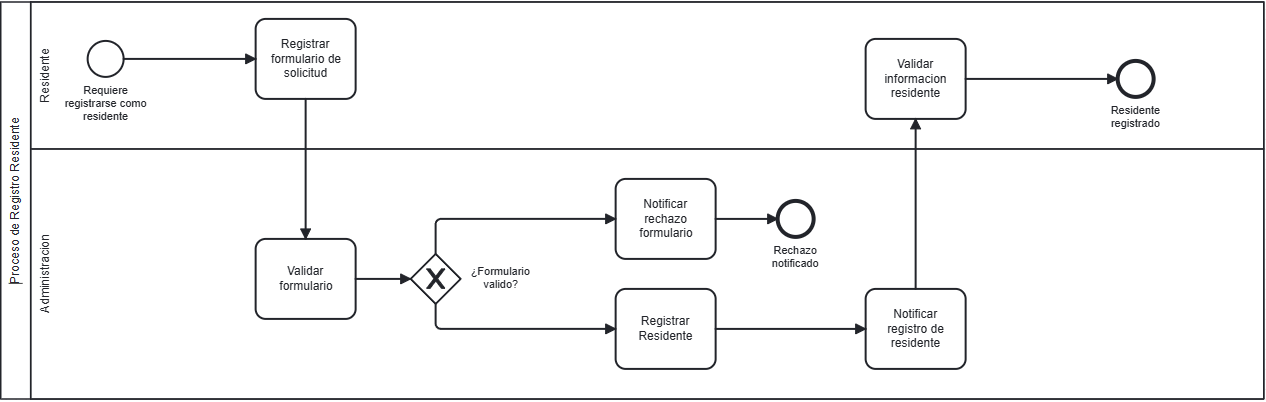
\includegraphics[width=0.95\linewidth]{ProcesoDeRegistroResidenteBPMN.png}
\caption{Proceso de registro de residente}
\label{fig:bpmn-inicio-sesion}
\end{figure}

\subsection{Proceso de registro de visitas}

El proceso de registro de visitas, común en comunidades sin plataformas digitales o con planes básicos de estas, comienza con la llegada del visitante al condominio. El conserje notifica la visita al residente y solicita la confirmación para autorizar el ingreso. Paralelamente, se solicita al visitante que complete un formulario en papel con sus datos personales y motivo de la visita. Una vez entregado el formulario al conserje, este procede a validar la información registrada. Tras la validación y la confirmación del residente, el conserje permite el ingreso del visitante, finalizando el proceso con su entrada al condominio.

\begin{figure}[H]
\centering
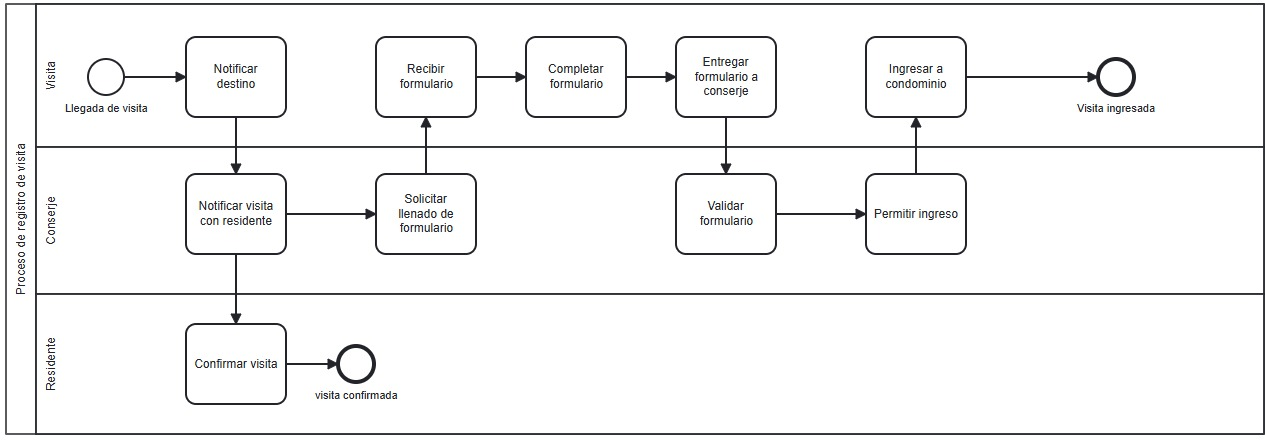
\includegraphics[width=0.95\linewidth]{ProcesoRegistroVisitaBPMN.jpg}
\caption{Proceso de registro de visitas en comunidades residenciales.}
\label{fig:bpmn-registro-visita}
\end{figure}

\subsection{Proceso de recepción y entrega de encomiendas}

El proceso de recepción de encomiendas, común en comunidades que no cuentan con plataformas digitales o utilizan planes básicos, comienza cuando un repartidor entrega el paquete a un conserje. Este registra manualmente la recepción, anotando los datos disponibles —como destinatario, remitente y hora de entrega— en un cuaderno o planilla física.

Luego de registrar la encomienda, el conserje notifica informalmente al residente, ya sea mediante una llamada telefónica, mensaje de texto o comunicación directa. El residente, al recibir la notificación, valida por su cuenta el envío con el proveedor para confirmar su origen y contenido. Una vez verificado, se dirige a retirar el paquete personalmente.

Finalmente, el residente firma un libro de recepción o documento similar como constancia de conformidad, completando así el proceso de entrega.


\begin{figure}[H]
\centering
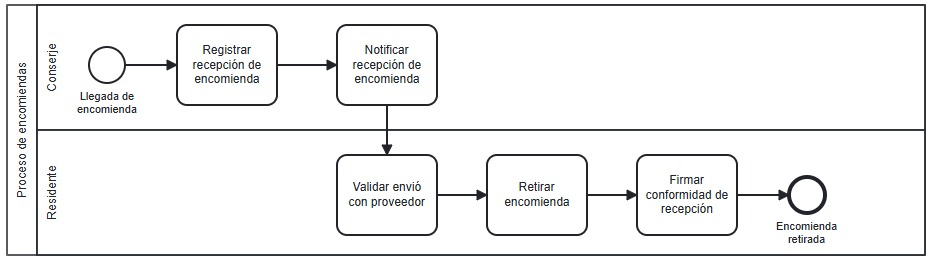
\includegraphics[width=0.95\linewidth]{ProcesoDeEncomiendasBPMN.jpg}
\caption{Proceso de encomiendas.}
\label{fig:bpmn-encomienda}
\end{figure}

\subsection{Proceso de pago de gastos comunes}

El proceso de pago de gastos comunes, tal como se realiza en muchas comunidades sin automatización digital, comienza con la llegada de la boleta mensual al residente, la cual suele ser enviada por correo electrónico o distribuida en formato físico (impresa). El residente revisa el detalle del cobro y, posteriormente, realiza una transferencia bancaria al número de cuenta indicado por la administración del edificio.

Una vez realizada la transferencia, el residente debe enviar manualmente el comprobante de pago —ya sea por correo electrónico, WhatsApp o entrega física— a la administración. Esta se encarga de validar el documento recibido, verificando el monto, la fecha y el nombre del remitente.

Si el pago es correcto, la administración actualiza el estado de los gastos comunes de manera manual en sus registros, y notifica al residente que su estado de cuenta ha sido actualizado. Finalmente, el residente puede comprobar que su boleta ha sido registrada como pagada, completando así el proceso.

\begin{figure}[H]
\centering
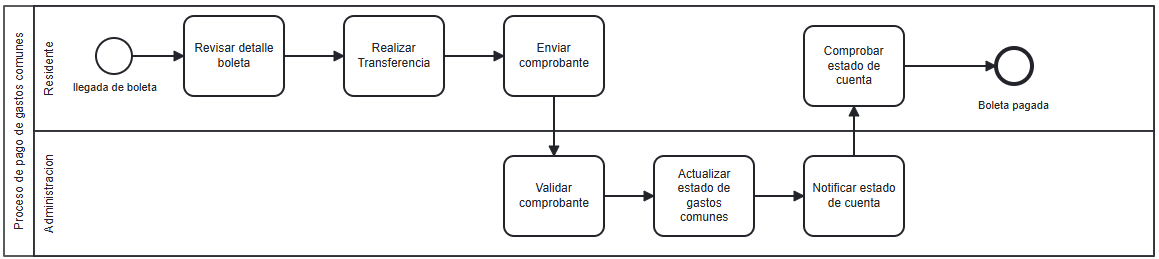
\includegraphics[width=0.95\linewidth]{ProcedoDePagoGgCcBPMN.png}
\caption{Proceso de pago de gastos comunes.}
\label{fig:bpmn-pago-ggcc}
\end{figure}

\subsection{Procesos digitalizados con DOMU}

Los diagramas anteriores representan los flujos manuales vigentes en comunidades sin plataformas digitales. A continuación se presentan los mismos cuatro procesos tal como son automatizados por DOMU, evidenciando la reducción de pasos manuales, la eliminación de papel y la incorporación de notificaciones en tiempo real.

\subsubsection{Registro de residente con DOMU}

Con DOMU, el registro de un nuevo residente se digitaliza completamente, eliminando formularios en papel y validaciones manuales. El sistema contempla dos modalidades de ingreso: un \textbf{registro autónomo}, donde el residente se inscribe directamente desde la plataforma, y un \textbf{registro por invitación}, donde el administrador envía un correo con un enlace de registro personalizado. En ambos casos, el sistema valida automáticamente la unicidad del email y el RUT antes de crear la cuenta. Tras la confirmación por correo electrónico, el administrador recibe una notificación con un enlace para aprobar o rechazar la solicitud mediante tokens seguros (\texttt{/approve/\{token\}} y \texttt{/reject/\{token\}}). Una vez aprobado, el administrador vincula al residente a una unidad habitacional específica, completando su incorporación a la comunidad. Este flujo reduce de 6~pasos manuales a un proceso mayormente automatizado, con intervención humana solo en la aprobación final.

% === PLACEHOLDER: BPMN TO-BE — Registro de Residente con DOMU ===
% PROMPT para generador de imágenes (Gemini/GPT/DALL-E):
%
% "Genera un DIAGRAMA BPMN 2.0 con swimlanes del proceso de registro de residente digitalizado con DOMU.
%
% NOTACIÓN BPMN 2.0 OBLIGATORIA:
% - EVENTOS INICIO: círculo fino verde (o negro) con borde simple.
% - EVENTOS FIN: círculo grueso negro con borde doble.
% - TAREAS: rectángulos redondeados con nombre de la tarea dentro.
% - GATEWAYS: diamantes (rombos) con X dentro para exclusivo, + para paralelo.
% - FLUJO DE SECUENCIA: flechas con línea sólida y punta llena.
% - FLUJO DE MENSAJE: flechas con línea PUNTEADA y punta abierta (entre swimlanes).
% - SWIMLANES: franjas horizontales separadas por líneas, nombre del participante a la izquierda en vertical.
%
% 3 SWIMLANES HORIZONTALES:
%
% SWIMLANE 'Residente':
% FLUJO 1 — Registro autónomo:
% ○ Inicio 'Requiere registrarse' → [Completa formulario en DOMU (nombre, email, RUT, comunidad)]
% → [Recibe correo de confirmación] → [Confirma email con clic en enlace] → [Espera aprobación del administrador]
% → ◉ Fin 'Cuenta activa y vinculada a unidad'
% FLUJO 2 — Registro por invitación (inicio alternativo):
% ○ Inicio 'Recibe invitación por correo del administrador' → [Accede al enlace de registro personalizado]
% → [Completa formulario pre-rellenado con datos de la invitación] → (continúa con confirmación de email)
%
% SWIMLANE 'Sistema DOMU':
% ◇ ¿Registro por invitación o autónomo? (gateway exclusivo al inicio)
%   → (Autónomo) [Valida datos y unicidad de email Y RUT] → ◇ ¿Datos válidos?
%     → (No) [Muestra errores de validación] → vuelve a formulario (flecha de retorno)
%     → (Sí) [Crea cuenta estado PENDIENTE] → [Envía correo confirmación con token]
%   → (Invitación) [Valida token de invitación] → [Pre-rellena formulario con datos de invitación]
%     → [Valida datos completados y unicidad email/RUT] → [Crea cuenta estado PENDIENTE]
% → [Recibe confirmación email] → [Genera token de aprobación y envía correo al administrador]
% → [Recibe respuesta del administrador (aprobación/rechazo)]
%   → (Aprobado) [Activa cuenta y asigna rol Residente]
%   → (Rechazado) [Marca cuenta como rechazada y notifica al solicitante]
% Flujos de mensaje (punteados): correo confirmación, clic confirmación, correo aprobación al admin.
%
% SWIMLANE 'Administrador':
% (Flujo de invitación — opcional):
% ○ Inicio 'Desea invitar residente' → [Envía invitación desde DOMU (/api/buildings/{id}/invite-admin)]
% → (flujo mensaje punteado al Residente)
% (Flujo de aprobación — siempre):
% [Recibe correo con enlace de aprobación] → ◇ ¿Aprueba solicitud?
%   → (Sí) [Aprueba con clic en enlace /approve/{token}] → [Asigna residente a unidad habitacional específica]
%     → ◉ Fin 'Residente asociado a comunidad'
%   → (No) [Rechaza con clic en enlace /reject/{token}] → ◉ Fin 'Solicitud rechazada'
%
% NOTA BPMN (rectángulo con esquina doblada):
% "Dos modalidades de ingreso: registro autónomo y registro por invitación del administrador.
% Aprobación/rechazo mediante tokens seguros por correo electrónico."
%
% ESTILO: Fondo blanco, swimlanes con fondo gris muy claro (#F8F8F8), bordes negros.
% Sin colores de relleno en las tareas (solo blanco). Tipografía sans-serif.
% Profesional para tesis universitaria. Etiquetas en español.
% Formato: PNG 300dpi orientación horizontal (landscape)."
\begin{figure}[H]
  \centering
  \fbox{\parbox{0.90\textwidth}{\centering\vspace{3cm}
  \textit{[Insertar diagrama BPMN: Proceso de registro de residente digitalizado con DOMU]}
  \vspace{3cm}}}
  \caption{Proceso de registro de residente --- digitalizado con DOMU.}
  \label{fig:bpmn-registro-tobe}
\end{figure}

Las Figuras~\ref{fig:screen-registro-formulario} y~\ref{fig:screen-registro-aprobacion} muestran capturas de pantalla del sistema DOMU correspondientes a este proceso.

\begin{figure}[H]
  \centering
  \fbox{\parbox{0.90\textwidth}{\centering\vspace{2.5cm}
  \textit{[Insertar captura de pantalla: Formulario de registro de residente en DOMU]}
  \vspace{2.5cm}}}
  \caption{Captura de pantalla --- Formulario de registro de residente en DOMU.}
  \label{fig:screen-registro-formulario}
\end{figure}

\begin{figure}[H]
  \centering
  \fbox{\parbox{0.90\textwidth}{\centering\vspace{2.5cm}
  \textit{[Insertar captura de pantalla: Correo de aprobación/rechazo recibido por el administrador]}
  \vspace{2.5cm}}}
  \caption{Captura de pantalla --- Correo electrónico de aprobación o rechazo de solicitud de registro.}
  \label{fig:screen-registro-aprobacion}
\end{figure}

\subsubsection{Registro de visitas con DOMU}

DOMU transforma el proceso de registro de visitas al eliminar el formulario en papel y la comunicación informal entre conserje y residente. La plataforma ofrece \textbf{tres modalidades de ingreso}: (1)~pre-autorización mediante código QR con vigencia temporal, que el visitante presenta al llegar; (2)~confirmación en tiempo real vía WebSocket, donde el residente aprueba o rechaza desde la aplicación; y (3)~\textbf{visita rápida} desde un contacto frecuente previamente registrado, que permite al conserje registrar el ingreso de forma instantánea sin QR ni confirmación. Los residentes pueden gestionar un directorio de contactos frecuentes (CRUD completo) para agilizar futuras visitas. El sistema registra tanto la hora de \textit{check-in} como la de \textit{check-out} en la bitácora digital, proporcionando trazabilidad completa del tiempo de permanencia. Esto reduce los 10~pasos manuales del proceso AS-IS a un flujo mayormente automatizado.

% === PLACEHOLDER: BPMN TO-BE — Registro de Visitas con DOMU ===
% PROMPT para generador de imágenes (Gemini/GPT/DALL-E):
%
% "Genera un DIAGRAMA BPMN 2.0 con swimlanes del proceso de registro de visitas digitalizado con DOMU.
%
% NOTACIÓN BPMN 2.0 OBLIGATORIA:
% - EVENTOS: ○ inicio (círculo fino), ◉ fin (círculo grueso doble).
% - TAREAS: rectángulos redondeados con nombre dentro.
% - GATEWAYS EXCLUSIVOS: diamantes (rombos) con X dentro y la pregunta como etiqueta.
% - FLUJO SECUENCIA: flechas sólidas. FLUJO MENSAJE: flechas punteadas entre lanes.
% - SWIMLANES: franjas horizontales, nombre del participante a la izquierda en vertical.
%
% 4 SWIMLANES HORIZONTALES:
%
% SWIMLANE 'Conserje':
% ○ Inicio 'Visitante llega' → ◇ ¿Modalidad de ingreso? (gateway exclusivo con 3 ramas)
%   → (QR pre-autorizado) [Escanea código QR de pre-autorización] → (flujo al Sistema para validación)
%     → [Registra check-in automático] → ◉ Fin 'Ingreso permitido'
%   → (Confirmación en tiempo real) [Escanea RUT con pistola QR] → [Selecciona residente destino en DOMU]
%     → (flujo mensaje punteado al Residente) → [Espera confirmación] → ◇ ¿Residente confirma?
%       → (Sí) [Registra check-in en DOMU] → ◉ Fin 'Ingreso permitido'
%       → (No) [Registra rechazo en bitácora] → ◉ Fin 'Acceso denegado'
%   → (Visita rápida) [Selecciona contacto frecuente del residente en DOMU]
%     → [Registro instantáneo sin QR ni confirmación (/api/visit-contacts/{id}/register)]
%     → ◉ Fin 'Ingreso permitido'
% (Al final de cada visita, sin importar modalidad):
% [Registra check-out cuando visitante se retira (/api/visits/{id}/checkout)] → ◉ Fin 'Visita cerrada'
%
% SWIMLANE 'Residente':
% (Flujo previo — gestión de contactos):
% [Gestiona contactos frecuentes en DOMU — CRUD completo (/api/visit-contacts)]
% (Flujo de pre-autorización):
% ○ Inicio 'Desea pre-autorizar' → [Ingresa datos del visitante en DOMU]
% → [Sistema genera QR temporal con vigencia definida]
% → [Envía QR al visitante por WhatsApp/email] → ◉ Fin 'QR enviado'
% (Flujo de confirmación en tiempo real):
% ← (recibe flujo de mensaje punteado del Conserje) → [Recibe notificación en tiempo real (WebSocket)]
% → [Confirma o rechaza visita desde la app] → (flujo mensaje punteado de vuelta al Conserje)
%
% SWIMLANE 'Sistema DOMU':
% [Valida QR y vigencia temporal] → ◇ ¿QR vigente?
%   → (Sí) [Autoriza ingreso automáticamente]
%   → (No) [Rechaza QR expirado, redirige a confirmación en tiempo real]
% [Envía notificación push/WebSocket al residente]
% [Registra check-in con timestamp en bitácora digital]
% [Registra check-out con timestamp en bitácora digital]
%
% NOTA BPMN (rectángulo con esquina doblada):
% "3 modalidades de ingreso: QR pre-autorizado con vigencia temporal,
% confirmación en tiempo real vía WebSocket, y visita rápida desde contacto frecuente.
% Se registra check-in y check-out con timestamp para trazabilidad completa."
%
% ESTILO: Fondo blanco, swimlanes gris muy claro, bordes negros, tareas blancas.
% Tipografía sans-serif. Profesional para tesis universitaria. Etiquetas en español.
% Formato: PNG 300dpi orientación horizontal (landscape)."
\begin{figure}[H]
  \centering
  \fbox{\parbox{0.90\textwidth}{\centering\vspace{3cm}
  \textit{[Insertar diagrama BPMN: Proceso de registro de visitas digitalizado con DOMU]}
  \vspace{3cm}}}
  \caption{Proceso de registro de visitas --- digitalizado con DOMU.}
  \label{fig:bpmn-visitas-tobe}
\end{figure}

Las Figuras~\ref{fig:screen-visitas-conserje},~\ref{fig:screen-visitas-contactos} y~\ref{fig:screen-visitas-notificacion} muestran capturas del sistema DOMU correspondientes a este proceso.

\begin{figure}[H]
  \centering
  \fbox{\parbox{0.90\textwidth}{\centering\vspace{2.5cm}
  \textit{[Insertar captura de pantalla: Vista del conserje --- registro de visita y escaneo de RUT/QR]}
  \vspace{2.5cm}}}
  \caption{Captura de pantalla --- Vista del conserje registrando una visita en DOMU.}
  \label{fig:screen-visitas-conserje}
\end{figure}

\begin{figure}[H]
  \centering
  \fbox{\parbox{0.90\textwidth}{\centering\vspace{2.5cm}
  \textit{[Insertar captura de pantalla: Gestión de contactos frecuentes del residente]}
  \vspace{2.5cm}}}
  \caption{Captura de pantalla --- Gestión de contactos frecuentes de visita en DOMU.}
  \label{fig:screen-visitas-contactos}
\end{figure}

\begin{figure}[H]
  \centering
  \fbox{\parbox{0.90\textwidth}{\centering\vspace{2.5cm}
  \textit{[Insertar captura de pantalla: Notificación en tiempo real de solicitud de visita]}
  \vspace{2.5cm}}}
  \caption{Captura de pantalla --- Notificación de confirmación de visita en tiempo real.}
  \label{fig:screen-visitas-notificacion}
\end{figure}

\subsubsection{Recepción y entrega de encomiendas con DOMU}

DOMU digitaliza completamente la gestión de encomiendas, reemplazando el cuaderno físico y las llamadas telefónicas por un flujo trazable con evidencia fotográfica. El conserje registra cada paquete tomando una \textbf{fotografía de evidencia} (paso central del flujo), la cual es automáticamente optimizada (redimensionada) y almacenada en Box con un identificador único. El ciclo de vida de cada encomienda sigue tres estados explícitos: \textbf{RECIBIDO}~$\rightarrow$~\textbf{NOTIFICADO}~$\rightarrow$~\textbf{RETIRADO}, y cada transición queda registrada con su \textit{timestamp} correspondiente. La notificación al residente se envía en \textbf{tiempo real mediante WebSocket}, permitiéndole visualizar la foto de evidencia directamente en la aplicación antes de acudir a retirar el paquete. Esto elimina los 5~pasos manuales del proceso AS-IS, incluyendo la firma en papel como constancia.

% === PLACEHOLDER: BPMN TO-BE — Encomiendas con DOMU ===
% PROMPT para generador de imágenes (Gemini/GPT/DALL-E):
%
% "Genera un DIAGRAMA BPMN 2.0 con swimlanes del proceso de encomiendas digitalizado con DOMU.
%
% NOTACIÓN BPMN 2.0 OBLIGATORIA:
% - EVENTOS: ○ inicio (círculo fino), ◉ fin (círculo grueso doble), ⏱ timer (círculo con reloj).
% - TAREAS: rectángulos redondeados con nombre dentro.
% - GATEWAYS: diamantes con X (exclusivo).
% - FLUJO SECUENCIA: flechas sólidas. FLUJO MENSAJE: flechas punteadas entre lanes.
% - SWIMLANES: franjas horizontales, nombre a la izquierda en vertical.
%
% 3 SWIMLANES HORIZONTALES:
%
% SWIMLANE 'Conserje':
% ○ Inicio 'Repartidor entrega paquete' → [Registra encomienda en DOMU (destinatario, descripción)]
% → [Toma fotografía de evidencia] → [Confirma registro]
% → (el sistema automáticamente optimiza, almacena foto y envía notificación -- flujo mensaje punteado)
% → ⏱ Timer 'Esperando retiro' → [Residente se presenta a retirar]
% → [Marca encomienda como RETIRADO en DOMU] → ◉ Fin 'Encomienda entregada'
%
% SWIMLANE 'Sistema DOMU':
% [Optimiza imagen (resize automático)] → [Almacena imagen en Box con ID único]
% → [Cambia estado a RECIBIDO con timestamp] → [Envía notificación WebSocket en tiempo real al residente]
% → [Cambia estado a NOTIFICADO con timestamp]
% → ... (espera retiro) ...
% → [Registra retiro con timestamp] → [Cambia estado a RETIRADO con timestamp]
%
% SWIMLANE 'Residente':
% [Recibe notificación en tiempo real (WebSocket)] → [Visualiza foto de evidencia en la app]
% → [Consulta detalle de encomienda] → [Se presenta en conserjería a retirar]
% → ◉ Fin 'Paquete retirado'
%
% NOTA BPMN (rectángulo con esquina doblada):
% "SIN cuaderno físico, SIN llamada telefónica, SIN firma en papel.
% Estados: RECIBIDO → NOTIFICADO → RETIRADO, cada transición con timestamp.
% Foto de evidencia optimizada y almacenada en Box."
%
% ESTILO: Fondo blanco, swimlanes gris muy claro, bordes negros, tareas blancas.
% Tipografía sans-serif. Profesional para tesis universitaria. Etiquetas en español.
% Formato: PNG 300dpi orientación horizontal (landscape)."
\begin{figure}[H]
  \centering
  \fbox{\parbox{0.90\textwidth}{\centering\vspace{3cm}
  \textit{[Insertar diagrama BPMN: Proceso de encomiendas digitalizado con DOMU]}
  \vspace{3cm}}}
  \caption{Proceso de recepción y entrega de encomiendas --- digitalizado con DOMU.}
  \label{fig:bpmn-encomienda-tobe}
\end{figure}

Las Figuras~\ref{fig:screen-encomienda-conserje} y~\ref{fig:screen-encomienda-residente} muestran capturas del sistema DOMU correspondientes a este proceso.

\begin{figure}[H]
  \centering
  \fbox{\parbox{0.90\textwidth}{\centering\vspace{2.5cm}
  \textit{[Insertar captura de pantalla: Vista del conserje registrando encomienda con fotografía de evidencia]}
  \vspace{2.5cm}}}
  \caption{Captura de pantalla --- Registro de encomienda con fotografía de evidencia en DOMU.}
  \label{fig:screen-encomienda-conserje}
\end{figure}

\begin{figure}[H]
  \centering
  \fbox{\parbox{0.90\textwidth}{\centering\vspace{2.5cm}
  \textit{[Insertar captura de pantalla: Vista del residente consultando encomienda con foto de evidencia]}
  \vspace{2.5cm}}}
  \caption{Captura de pantalla --- Vista del residente con detalle de encomienda y foto de evidencia.}
  \label{fig:screen-encomienda-residente}
\end{figure}

\subsubsection{Pago de gastos comunes con DOMU}

DOMU automatiza la gestión financiera de gastos comunes eliminando las planillas manuales, las transferencias sin trazabilidad y la validación manual de comprobantes. El sistema calcula los cargos por unidad habitacional utilizando un \textbf{coeficiente de prorrata} específico, y genera tres tipos de documentos PDF mediante servicios especializados: \textit{estado de cuenta general} (\texttt{CommonExpensePdfService}), \textit{comprobante de pago} (\texttt{PaymentReceiptPdfService}) y \textit{detalle de cargo individual} (\texttt{ChargeReceiptPdfService}). El residente puede \textbf{seleccionar cargos específicos a pagar} (pago parcial), sin necesidad de saldar todos los pendientes simultáneamente. Además, como alternativa al pago en línea, el residente puede \textbf{subir un comprobante de transferencia bancaria} como imagen, el cual queda asociado al pago para revisión del administrador. El administrador dispone de un panel financiero para listar y filtrar pagos por período, unidad y estado, y puede descargar reportes PDF de cada período. En la versión~1.0, DOMU opera con una pasarela de pago simulada; el comprobante de transferencia sirve como alternativa funcional.

% === PLACEHOLDER: BPMN TO-BE — Pago de Gastos Comunes con DOMU ===
% PROMPT para generador de imágenes (Gemini/GPT/DALL-E):
%
% "Genera un DIAGRAMA BPMN 2.0 con swimlanes del proceso de pago de gastos comunes digitalizado con DOMU.
%
% NOTACIÓN BPMN 2.0 OBLIGATORIA:
% - EVENTOS: ○ inicio (círculo fino), ◉ fin (círculo grueso doble).
% - TAREAS: rectángulos redondeados con nombre dentro. Tareas automáticas (sistema) con ícono de engranaje.
% - GATEWAYS EXCLUSIVOS: diamantes con X dentro.
% - FLUJO SECUENCIA: flechas sólidas. FLUJO MENSAJE: flechas punteadas entre lanes.
% - SWIMLANES: franjas horizontales, nombre a la izquierda en vertical.
% - ARTEFACTO (documento): ícono de documento con esquina doblada para representar PDFs generados.
%
% 3 SWIMLANES HORIZONTALES:
%
% SWIMLANE 'Administrador':
% ○ Inicio 'Cierre período mensual' → [Crea período de gasto común en DOMU]
% → [Carga cargos por unidad (prorrateo automático con coeficiente)] → (flujo al Sistema)
% → ... (más adelante) [Revisa pagos pendientes por unidad en panel financiero]
% → [Filtra pagos por período, unidad y estado]
% → [Descarga reporte PDF de período] 📄 → ◉ Fin 'Período cerrado'
%
% SWIMLANE 'Sistema DOMU':
% [Calcula cargos con coeficiente de prorrata por unidad habitacional]
% → [Genera 3 tipos de PDF (OpenPDF):] 📄📄📄
%    - 📄 Estado de cuenta general (CommonExpensePdfService)
%    - 📄 Comprobante de pago (PaymentReceiptPdfService)
%    - 📄 Detalle de cargo individual (ChargeReceiptPdfService)
% → [Envía notificación WebSocket de nuevo cobro a residentes]
% → ... → [Recibe pago o comprobante de transferencia del residente]
% → ◇ ¿Tipo de pago?
%   → (Pago en línea - pasarela simulada v1.0) → ◇ ¿Pago correcto?
%     → (Sí) [Registra pago y actualiza estado] → [Genera comprobante PDF] 📄 → [Notifica confirmación]
%     → (No) [Rechaza pago y muestra error]
%   → (Comprobante de transferencia) [Almacena comprobante de transferencia subido por residente]
%     → [Asocia comprobante al pago para revisión del administrador] → [Notifica al administrador]
%
% SWIMLANE 'Residente':
% [Recibe notificación de nuevo estado de cuenta (WebSocket)] → [Consulta cartola en la app]
% → [Descarga PDF de estado de cuenta] → [Selecciona cargos específicos a pagar (puede pagar parcialmente)]
% → ◇ ¿Medio de pago?
%   → (Pago en línea) [Inicia flujo de pago en DOMU] → [Confirma transacción]
%     → [Recibe comprobante PDF por email] → ◉ Fin 'Pago registrado'
%   → (Transferencia bancaria) [Realiza transferencia bancaria externa]
%     → [Sube comprobante de transferencia como imagen (/api/payments/upload-receipt)]
%     → ◉ Fin 'Comprobante enviado, pendiente de revisión'
%
% ARTEFACTOS PDF (mostrar como documentos BPMN adjuntos al proceso):
% 📄 Estado de cuenta — 📄 Comprobante de pago — 📄 Detalle de cargo
%
% NOTA BPMN (rectángulo con esquina doblada):
% "SIN boletas en papel, SIN WhatsApp para enviar comprobantes, SIN validación manual.
% v1.0 opera con pasarela simulada; comprobante de transferencia como alternativa.
% 3 PDFs generados: estado de cuenta, comprobante de pago, detalle de cargo."
%
% ESTILO: Fondo blanco, swimlanes gris muy claro, bordes negros, tareas blancas.
% Tipografía sans-serif. Profesional para tesis universitaria. Etiquetas en español.
% Formato: PNG 300dpi orientación horizontal (landscape)."
\begin{figure}[H]
  \centering
  \fbox{\parbox{0.90\textwidth}{\centering\vspace{3cm}
  \textit{[Insertar diagrama BPMN: Proceso de pago de gastos comunes digitalizado con DOMU]}
  \vspace{3cm}}}
  \caption{Proceso de pago de gastos comunes --- digitalizado con DOMU.}
  \label{fig:bpmn-pago-tobe}
\end{figure}

Las Figuras~\ref{fig:screen-pago-pdf},~\ref{fig:screen-pago-residente} y~\ref{fig:screen-pago-admin} muestran capturas del sistema DOMU correspondientes a este proceso.

\begin{figure}[H]
  \centering
  \fbox{\parbox{0.90\textwidth}{\centering\vspace{2.5cm}
  \textit{[Insertar captura de pantalla: PDF de estado de cuenta generado por DOMU]}
  \vspace{2.5cm}}}
  \caption{Captura de pantalla --- Estado de cuenta en PDF generado por DOMU.}
  \label{fig:screen-pago-pdf}
\end{figure}

\begin{figure}[H]
  \centering
  \fbox{\parbox{0.90\textwidth}{\centering\vspace{2.5cm}
  \textit{[Insertar captura de pantalla: Vista del residente pagando o subiendo comprobante de transferencia]}
  \vspace{2.5cm}}}
  \caption{Captura de pantalla --- Flujo de pago del residente y subida de comprobante de transferencia.}
  \label{fig:screen-pago-residente}
\end{figure}

\begin{figure}[H]
  \centering
  \fbox{\parbox{0.90\textwidth}{\centering\vspace{2.5cm}
  \textit{[Insertar captura de pantalla: Panel financiero del administrador con pagos por unidad]}
  \vspace{2.5cm}}}
  \caption{Captura de pantalla --- Panel financiero del administrador en DOMU.}
  \label{fig:screen-pago-admin}
\end{figure}

La comparación entre los diagramas de procesos manuales y digitalizados evidencia que DOMU elimina la dependencia de registros en papel, reduce los puntos de contacto manual y garantiza la trazabilidad de cada operación mediante notificaciones automáticas y almacenamiento digital.

\section{Propuesta de Solución}

Se propone una plataforma web que centralice los procesos críticos de la administración de copropiedades, desde el control de accesos hasta la gestión financiera y la comunicación interna.

A diferencia de las herramientas actuales, \textit{DOMU} integra un sistema de registro de visitas que permite a los residentes pre-autorizar visitantes, crear contactos frecuentes y agendar visitas con fecha y hora. La conserjería puede verificar el ingreso mediante códigos QR, validar el RUT y registrar el \textit{check-in}, facilitando el control y la trazabilidad de accesos sin depender de dispositivos físicos especializados.

Asimismo, la plataforma digitaliza el registro de encomiendas, la gestión de incidentes y reclamos con seguimiento por estado y asignación, y la reserva de áreas comunes con control de aforo, franjas horarias y bloqueo ante morosidad. El módulo financiero permite crear períodos de gastos comunes, cargar cargos, generar estados de cuenta en PDF y habilitar un flujo de pago que registra comprobantes y emite recibos.

La comunicación interna se apoya en un foro categorizado, un chat en tiempo real entre vecinos y una tienda comunitaria para compraventa dentro del edificio. Los residentes pueden participar en votaciones con cierre programado y exportación de resultados, y los administradores pueden gestionar personal, gestionar proveedores, asignar tareas y administrar unidades habitacionales y residentes desde un mismo entorno.

De este modo, la aplicación aborda de manera unificada la administración interna (tareas y personal), la experiencia del residente (pagos, reservas, comunicación, incidentes) y la transparencia financiera, promoviendo eficiencia y coordinación en la convivencia diaria.

\section{Análisis de los principales trabajos realizados en el área}

Actualmente existen varias soluciones orientadas a la administración de edificios y condominios, como \textit{ComunidadFeliz}, \textit{Edifito}, \textit{Edipro} y \textit{GastoComunChile}. Todas ellas abordan parcialmente la gestión financiera, la comunicación con residentes, el registro de gastos comunes y, en algunos casos, el control de accesos. Sin embargo, ninguna integra de forma completa las áreas involucradas —administrador, residentes, personal de aseo, conserjes, proveedores y visitas.

\begin{enumerate}
    \item \textbf{ComunidadFeliz}~\cite{comunidadfeliz2025}: ofrece una plataforma enfocada en la administración digital de comunidades residenciales, con funcionalidades que incluyen gestión de gastos comunes, pagos en línea, comunicación con residentes, votaciones virtuales, reservas de espacios comunes y conciliación bancaria. El Plan Full incorpora módulos adicionales como gestión de conserjería, remuneraciones y soporte especializado.

    \par\noindent
    Si bien \textit{ComunidadFeliz} cuenta con una presencia consolidada en el mercado chileno, su enfoque se centra principalmente en la administración financiera y la interacción con residentes, dejando fuera la integración operativa directa de actores como el personal interno, proveedores o sistemas físicos de acceso.

    \begin{figure}[H]
        \centering
        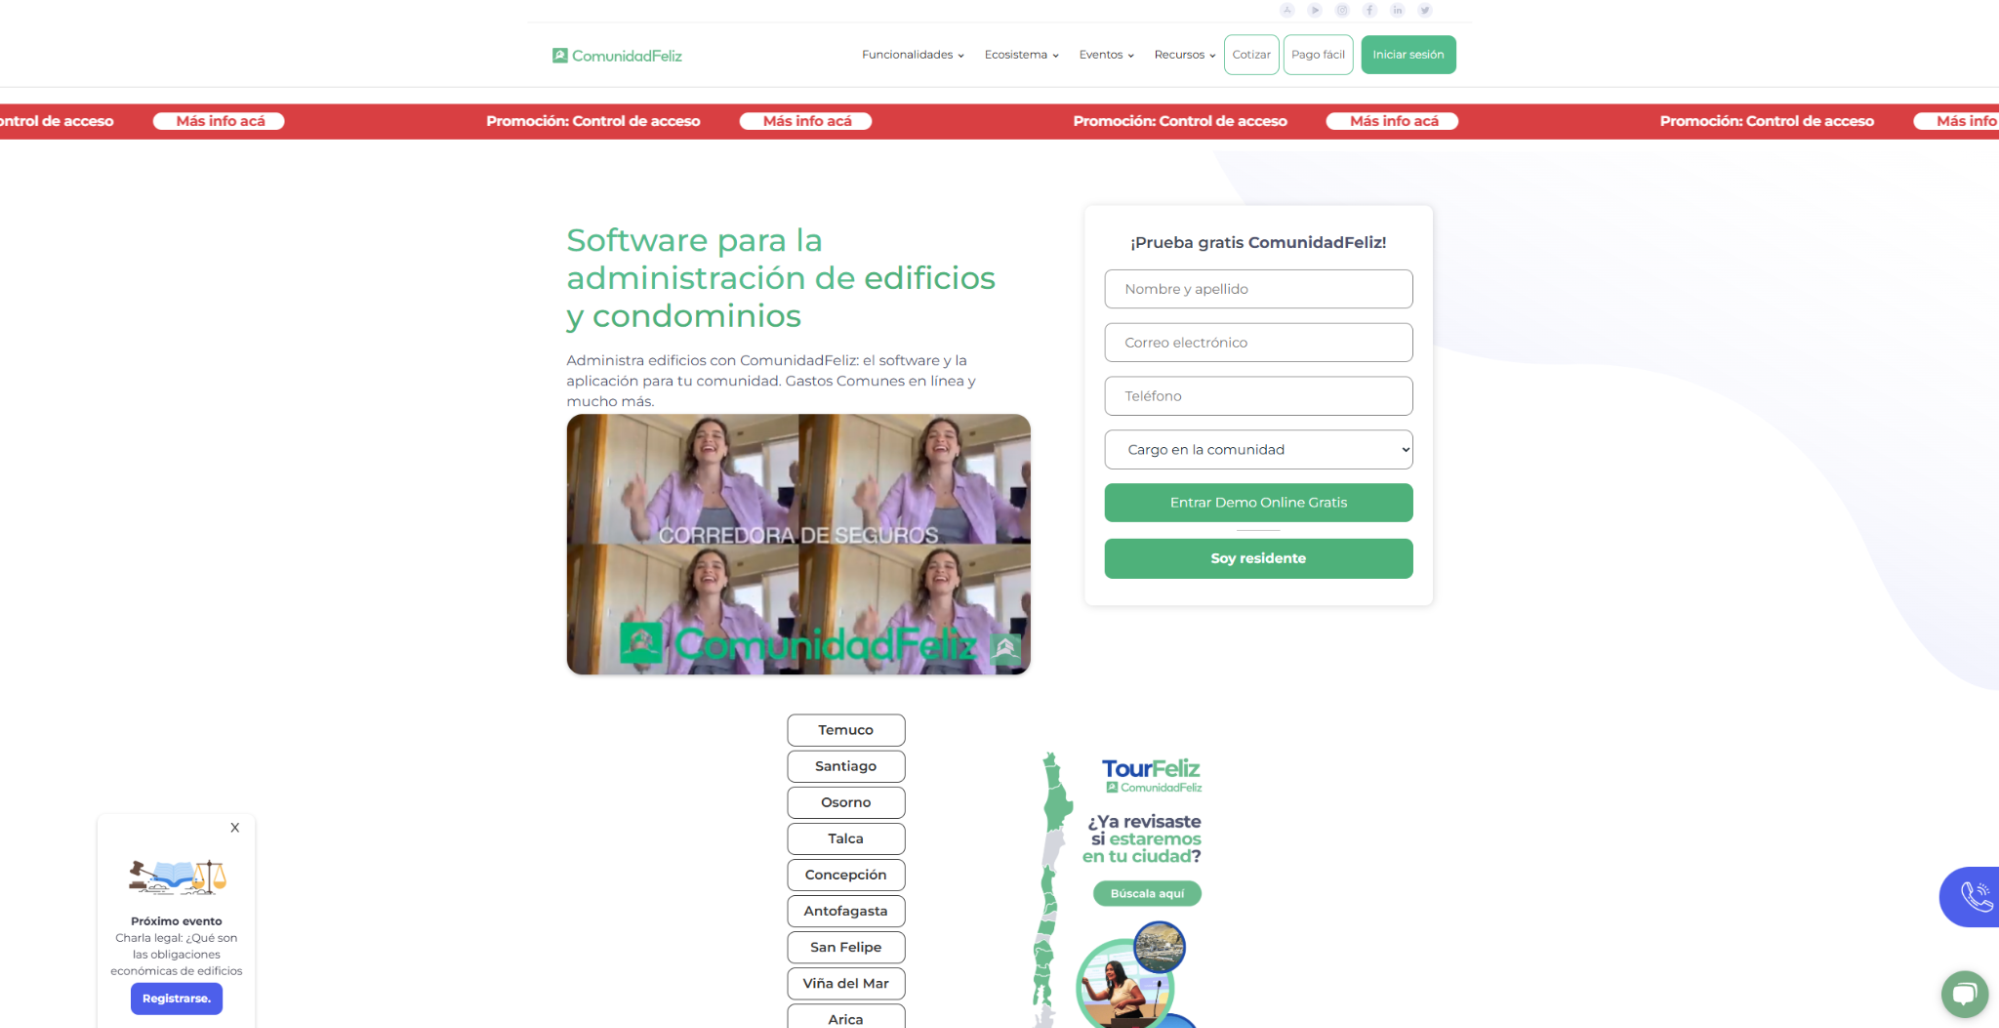
\includegraphics[width=.8\linewidth]{PaginaComunidadFeliz.png}
        \caption{Página web de ComunidadFeliz.}
        \label{fig:site-comunidadfeliz}
    \end{figure}

    \item \textbf{Edifito}~\cite{edifito2025}: ofrece una plataforma digital orientada a la administración integral de comunidades, con foco en la automatización de procesos financieros y operativos. Entre sus principales funcionalidades se encuentran la generación automática de gastos comunes, conciliación bancaria, gestión de remuneraciones, control de accesos mediante códigos QR o lectura de cédulas —similar a los lectores de precios de las cajas automáticas de supermercados—, administración de encomiendas, reservas de espacios comunes, comunicación interna, votaciones virtuales y conexión con cámaras de seguridad.

    \par\noindent
    \textit{Edifito} trabaja bajo un modelo comercial basado exclusivamente en cotización personalizada, por lo que no publica valores estándar en su sitio web. El precio final se ajusta en función del tamaño de la comunidad, la cantidad de unidades habitacionales y los módulos requeridos por cada cliente.

    \begin{figure}[H]
        \centering
        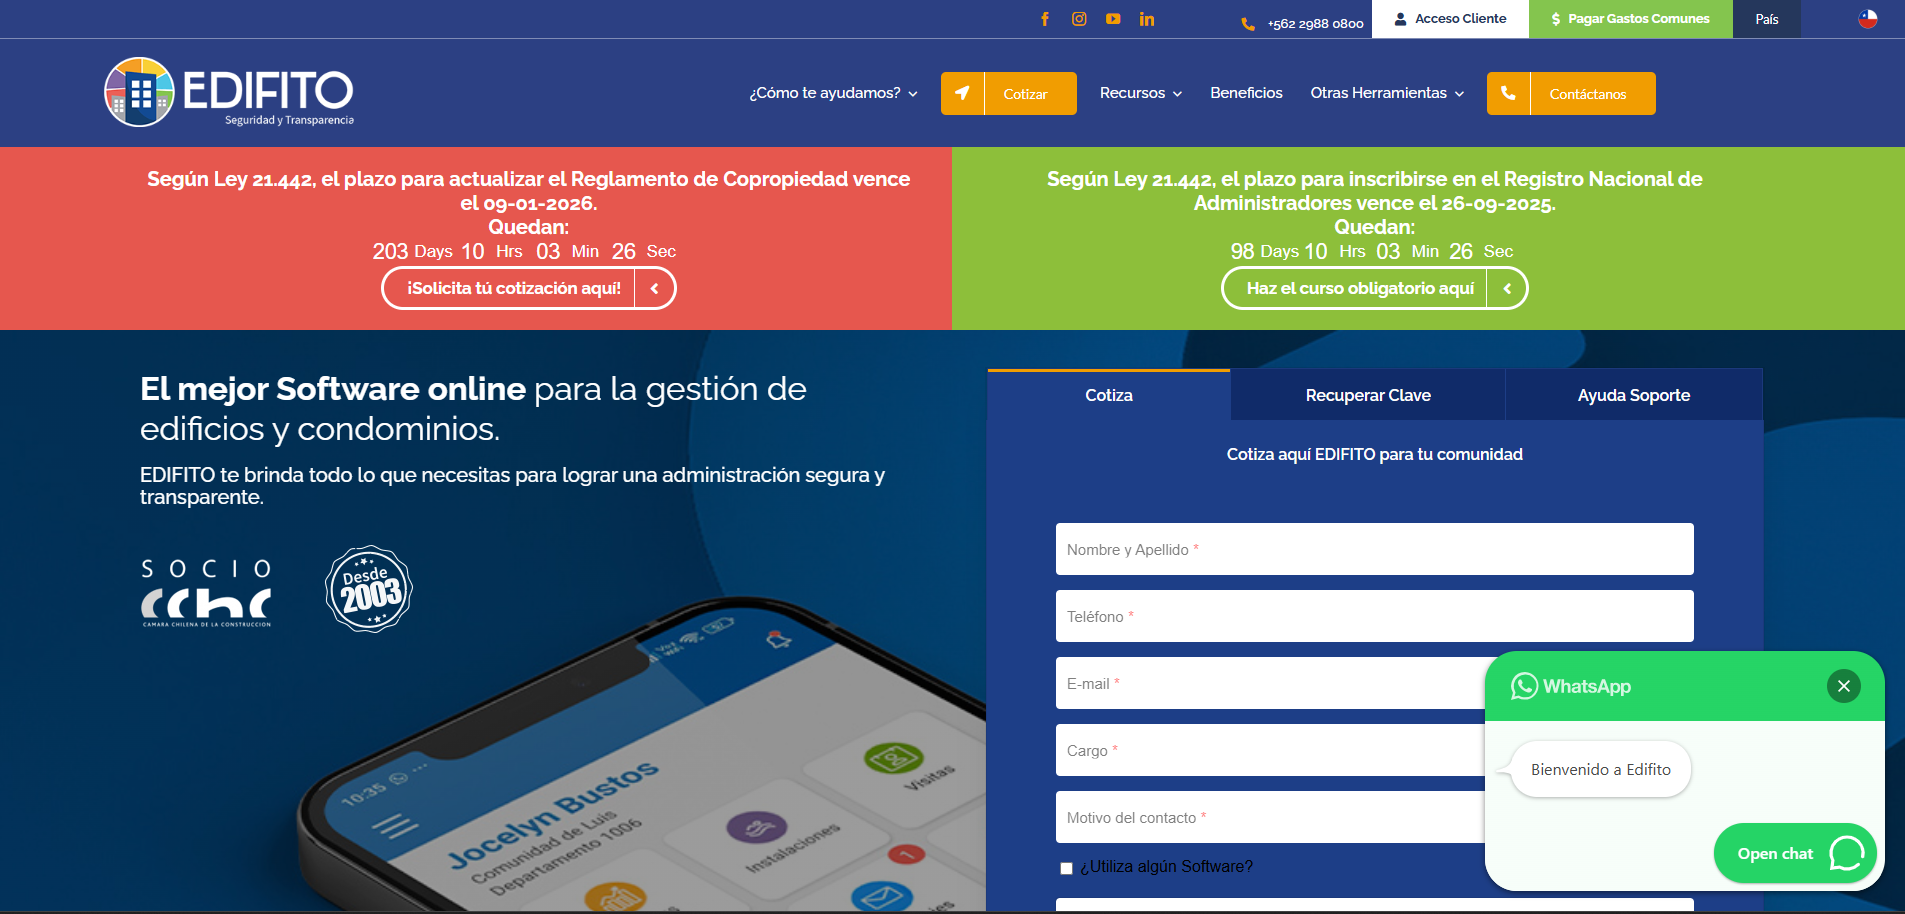
\includegraphics[width=.8\linewidth]{PaginaEdifito.png}
        \caption{Página web de Edifito.}
        \label{fig:site-edifito}
    \end{figure}

    \item \textbf{Edipro}~\cite{edipro2025}: ofrece una plataforma digital orientada a la administración de comunidades, centrada principalmente en la automatización de procesos financieros y operativos. Sus funcionalidades incluyen gestión de gastos comunes, conciliación bancaria, control de accesos mediante códigos QR o lectura de cédulas, administración de remuneraciones, registro de encomiendas, reservas de espacios comunes, votaciones virtuales, comunicación interna, videoconferencias e integración con cámaras de seguridad.

    \par\noindent
    \textit{Edipro} opera bajo un modelo modular, compuesto por tres paquetes escalables según las necesidades de cada comunidad. El \textit{Pack Conserje} (CLP 9.571 mensuales) contempla funciones básicas como control de accesos, registro de visitas y encomiendas, mensajería interna y tareas operativas. El \textit{Pack Administra} (CLP 25.524 mensuales) añade contabilidad, cálculo de gastos comunes, remuneraciones y conciliación bancaria. Finalmente, el \textit{Pack Full} (aproximadamente CLP 31.905 mensuales) integra todos los servicios anteriores, sumando reservas de espacios, videoconferencias y votaciones digitales.

    \par\noindent
    Estos valores se encuentran disponibles en el portal oficial:       \url{https://www.comparasoftware.cl/edipro}.

    \begin{figure}[H]
        \centering
        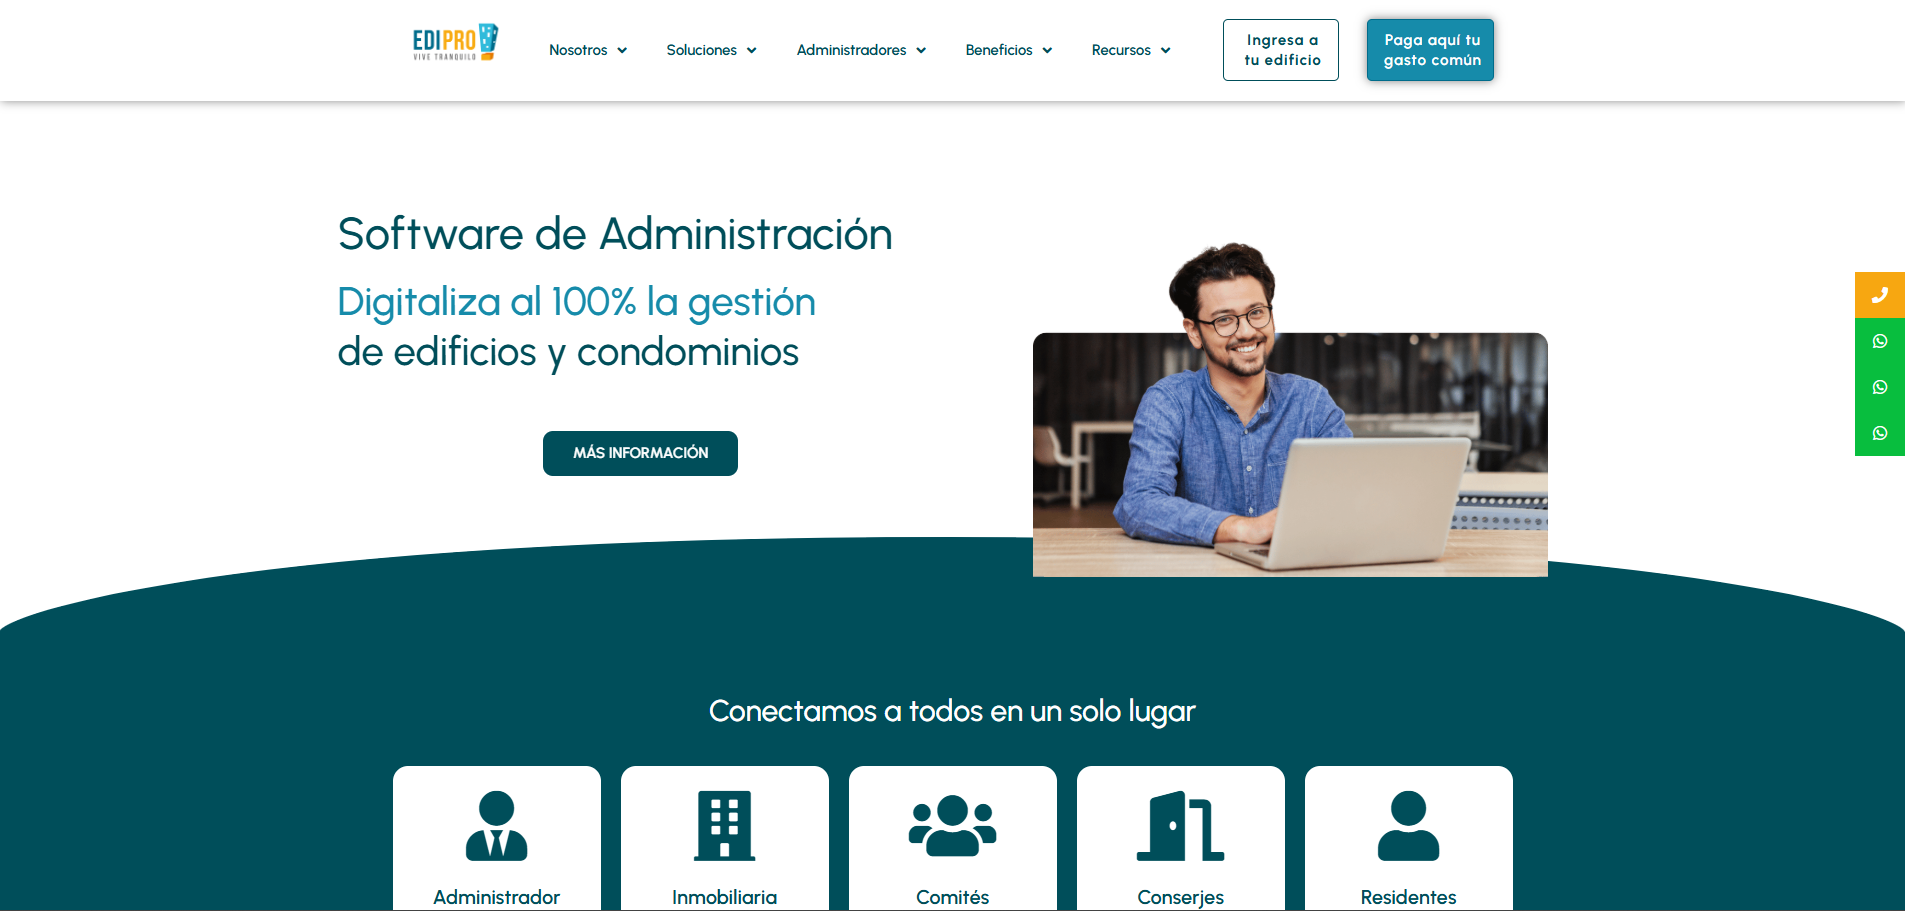
\includegraphics[width=.8\linewidth]{PaginaEdipro.png}
        \caption{Página web de Edipro.}
        \label{fig:site-edipro}
    \end{figure}


    \item \textbf{GastoComunChile}~\cite{gastocomunchile2025}: su propuesta se centra en optimizar la gestión financiera comunitaria, con funcionalidades que incluyen el ingreso de consumos y cobros individuales, cálculo automático de gastos comunes, conciliación bancaria, generación de minutas y reportes —como libro diario, mayor, cartolas de morosidad o corte de servicios—, envío masivo de notificaciones por correo y gestión de remuneraciones con archivos compatibles con \textit{Previred}.

    \par\noindent
    \textit{GastoComunChile} ofrece planes por comunidad con un costo inicial de \$25.000 CLP al mes (más IVA), o \$250.000 CLP al año si se prefiere pago anual, incluyendo soporte técnico, configuración personalizada y actualizaciones continuas sin cargo adicional.

    \par\noindent
    Aunque la plataforma cubre a fondo toda la gestión de gastos comunes y nómina, se posiciona como una competencia fuerte únicamente en ese ámbito específico.

    \begin{figure}[H]
        \centering
        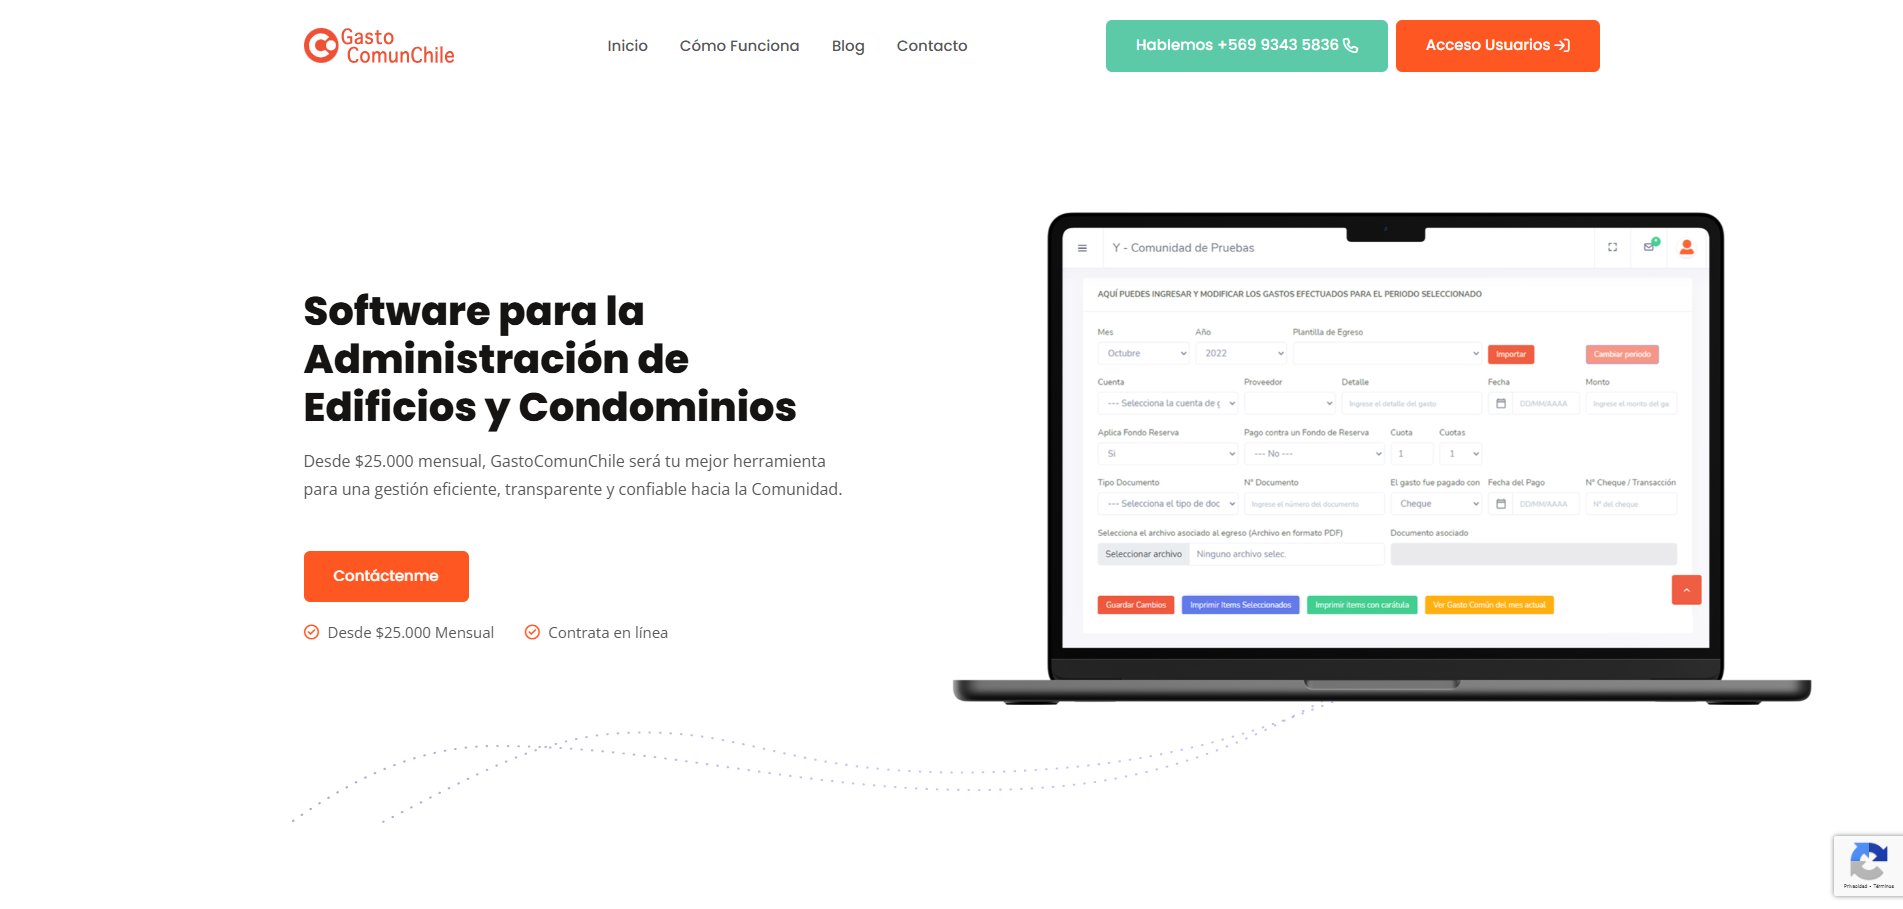
\includegraphics[width=.8\linewidth]{PaginaGastoComunChile.png}
        \caption{Página web de GastoComunChile.}
        \label{fig:site-gastocomunchile}
    \end{figure}

\end{enumerate}

\par\vspace{0.5em}
\noindent
\textit{DOMU} se diferencia al proponer un sistema integral que combina la plataforma de software con un sistema de acceso ágil, automatizando el registro de visitantes, proveedores y personal de mantenimiento. Además, incorpora la gestión centralizada de tareas, pagos, comunicación interna y votaciones en un solo entorno, solucionando la falta de trazabilidad y coordinación observada en los sistemas actuales.


\section{Justificación de la Propuesta}

La gestión de comunidades residenciales involucra una serie de procesos interdependientes: el control de accesos, la administración financiera, la comunicación con residentes, la recepción de encomiendas y la coordinación del personal interno. En la práctica, muchas de estas tareas se realizan de forma fragmentada (mediante planillas, correos electrónicos o plataformas digitales aisladas), lo que genera ineficiencias, errores frecuentes, pérdida de tiempo y una limitada capacidad de control y trazabilidad. La desconexión entre módulos impide que administradores, conserjes y residentes compartan una misma visión del estado de la comunidad y de las acciones pendientes.

Las plataformas existentes han digitalizado aspectos específicos (gestión financiera, comunicación, reservas o accesos), sirviendo como referencia para identificar buenas prácticas. Sin embargo, la mayoría de ellas opera de forma modular o con enfoque parcial: algunas priorizan el área financiera y descuidan la operativa; otras facilitan el control de accesos pero no integran la gestión de encomiendas, incidentes o tareas internas. Esta ausencia de integración limita su efectividad para ofrecer una experiencia realmente centralizada, segura y eficiente en la comunidad.

En este contexto, la propuesta de \textit{DOMU} se justifica por su enfoque integral, centrado en una única plataforma que conecta los procesos críticos de la administración comunitaria. En lugar de depender de dispositivos físicos especializados, el sistema aprovecha el computador de conserjería y la web para permitir que los residentes pre-autoricen visitas, gestionen contactos frecuentes y que la portería verifique el ingreso mediante códigos QR y validación de RUT. Esta aproximación reduce errores de transcripción y mejora la trazabilidad sin requerir hardware adicional.

El control de accesos se complementa con la gestión de encomiendas (recepción, asignación a unidad y cambio de estado hasta la entrega), la gestión de incidentes y reclamos con seguimiento por estado y asignación, y la reserva de áreas comunes con control de aforo, franjas horarias y bloqueo ante morosidad. El módulo financiero permite crear períodos de gastos comunes, cargar cargos, generar estados de cuenta en PDF y registrar pagos con comprobantes y recibos. La comunicación interna se apoya en un foro categorizado, un chat en tiempo real entre vecinos y una tienda comunitaria para compraventa dentro del edificio. Además, el sistema permite asignar y monitorear tareas del personal, realizar votaciones con cierre programado y administrar unidades habitacionales y residentes desde un mismo entorno.

\textit{DOMU} no solo digitaliza procesos aislados, sino que los centraliza y conecta en un solo sistema, entregando una solución moderna, escalable y competitiva frente a las herramientas actuales. Su implementación apunta a mejorar la eficiencia administrativa, fortalecer el control y la transparencia, y promover una mejor convivencia en los entornos residenciales.

\section{Objetivos del proyecto}

En este punto se presentan los objetivos que guiarán el desarrollo, junto con las actividades correspondientes para su cumplimiento. Se expone tanto el objetivo general como los objetivos específicos.

\subsection{Objetivo General del proyecto}

Desarrollar una plataforma web integral para la administración de comunidades residenciales que integre y optimice los procesos críticos: registro y verificación de visitas con pre-autorización y control de acceso, trazabilidad de encomiendas, gestión de gastos comunes con generación de estados de cuenta y registro de pagos, asignación y seguimiento de tareas al personal, reporte y seguimiento de incidentes, reserva de áreas comunes, y comunicación interna mediante foro, chat y marketplace comunitario. El sistema debe ofrecer un entorno centralizado, trazabilidad de la información y acceso continuo para administradores, conserjes y residentes.


\subsection{Objetivos Específicos y Descripción de las actividades}

A continuación, se detallan los objetivos específicos del proyecto junto con  la descripción de las actividades asociadas a cada uno de estos. Estas actividades permitirán organizar de manera estructurada las tareas necesarias para alcanzar los objetivos planteados, asegurando un desarrollo sistemático y organizado del proyecto.
\newpage
\begin{longtable}{|p{0.4\textwidth}|p{0.55\textwidth}|}
\hline
\textbf{Objetivo} & \textbf{Descripción de las actividades} \\
\hline
\endfirsthead

\hline
\textbf{Objetivo} & \textbf{Descripción de las actividades} \\
\hline
\endhead

\hline
\endfoot

\hline
1. Comparar los sistemas actuales de administración de edificios, identificando sus fortalezas y limitaciones, así como las percepciones de los usuarios, para definir los requerimientos funcionales de nuestra propuesta. &
\begin{enumerate}
    \item Investigar y documentar al menos tres sistemas de administración de edificios existentes en el mercado chileno.
    \item Identificar las características y funcionalidades clave de cada sistema, considerando también la experiencia de uso reportada por los usuarios finales.
    \item Analizar las fortalezas y debilidades de cada sistema en relación con las necesidades detectadas de los distintos tipos de usuarios (administradores, residentes, personal).
    \item Recoger y sistematizar retroalimentación de usuarios reales mediante encuestas o entrevistas estructuradas (mínimo 5 personas).
    \item Definir los requerimientos funcionales del nuevo sistema basándose en el análisis comparativo y en las necesidades expresadas por los usuarios.
\end{enumerate}
\\ \hline

2. Definir tecnologías y metodologías disponibles que permitan desarrollar el sistema de registro con escaneo QR, página web y backend. &
\begin{enumerate}
    \item Definir tecnologías para el frontend y backend.
    \item Investigar y seleccionar el hardware de escaneo QR (pistola lectora), evaluando su compatibilidad  y la estructura de datos arrojada por la cédula de identidad chilena.
    \item Evaluar metodologías de desarrollo de software (ágil, cascada, etc.) adecuadas para el proyecto y escoger la que mejor se ajuste a la propuesta.
    \item Investigar opciones para la integración \textit{plug-and-play} del escáner QR con el computador de conserjería, y definir el método de procesamiento de la cadena de texto obtenida.
\end{enumerate}
\\ \hline

3. Diseñar la estructura de software que incorpora módulos de control de acceso, seguimiento de encomiendas, asignación de tareas al personal y comunicación con los residentes, entre otros. &
\begin{enumerate}
    \item Definir la arquitectura general del software y sus diferentes módulos.
    \item Diseñar el modelo de datos para cada módulo.
    \item Diseñar los diagramas de procesos en notación BPMN y los modelos entidad–relación (MER) correspondientes a los flujos.
    \item Diseñar la interfaz de usuario (UI) para cada módulo.
\end{enumerate}
\\ \hline

4. Implementar un prototipo funcional que integre los módulos diseñados en una plataforma inicial. &
\begin{enumerate}
    \item Configurar el entorno de desarrollo y las herramientas de control de versiones.
    \item Implementar las funcionalidades de backend.
    \item Desarrollar el frontend garantizando la comunicación con el backend.
    \item Realizar pruebas unitarias y ajustes.
    \item Asegurar la correcta sincronización de datos entre módulos.
\end{enumerate}
\\ \hline

5. Integrar el software de registro con el hardware de escaneo QR, verificando la correcta captura, \textit{parseo} y envío de los datos de la cédula de identidad a la plataforma central. &
\begin{enumerate}
    \item Adquirir el hardware (pistola escáner) y configurar los \textit{drivers} necesarios para la correcta \textit{emulación del teclado} en el computador de conserjería.
    \item Implementar la lógica de \textit{parsing} (análisis) en el software para decodificar la cadena de texto arrojada por el escáner QR de la cédula chilena.
    \item Garantizar la sincronización y el envío seguro de los datos personales capturados a la base de datos central.
    \item Validar la precisión de la captura y el \textit{parsing} de los campos de la cédula (RUT, Nombre, Apellido).
    \item Realizar pruebas de rendimiento y robustez del proceso de escaneo.
\end{enumerate}
\\ \hline

6. Realizar pruebas finales, validación y ajuste del sistema DOMU. &
\begin{enumerate}
    \item Diseñar un plan de pruebas integral.
    \item Recopilar retroalimentación de usuarios finales.
    \item Corregir y optimizar el sistema según resultados.
    \item Validar cumplimiento de requerimientos definidos.
    \item Documentar resultados y dejar el sistema operativo.
\end{enumerate}
\\ \hline

\end{longtable}

\section{Composición del Informe}
El presente informe se organiza en nueve capítulos que abordan las distintas etapas del proyecto. A continuación se describe brevemente el contenido de cada uno:

\begin{itemize}
    \item \textbf{Capítulo 1 -- Introducción:} presenta el contexto del proyecto, la problemática identificada, los procesos actuales del ámbito, la propuesta de solución, el análisis de trabajos relacionados, la justificación, los objetivos y la composición del informe.

    \item \textbf{Capítulo 2 -- Proyecto:} describe los objetivos del software, la metodología de desarrollo adoptada, las tecnologías, herramientas y frameworks utilizados, y los estándares de documentación aplicados.

    \item \textbf{Capítulo 3 -- Especificación de Requerimientos:} detalla los límites del proyecto y los requerimientos funcionales y no funcionales del sistema, agrupados por módulo.

    \item \textbf{Capítulo 4 -- Factibilidad del Proyecto:} evalúa la viabilidad técnica, operativa y económica de la propuesta, proporcionando una base para la toma de decisiones estratégicas.

    \item \textbf{Capítulo 5 -- Análisis del Proyecto:} presenta los casos de uso que modelan la interacción entre los actores y el sistema.

    \item \textbf{Capítulo 6 -- Diseño:} aborda los servicios web, el modelo de datos, los diagramas entidad-relación, la arquitectura del software y el diseño de las interfaces de usuario.

    \item \textbf{Capítulo 7 -- Desarrollo del Trabajo:} detalla la estructura del código fuente, la configuración del entorno, las fases de implementación y los aspectos técnicos más relevantes de la solución.

    \item \textbf{Capítulo 8 -- Implantación y Puesta en Marcha:} describe la estrategia de despliegue en un entorno productivo, la arquitectura basada en contenedores y la adopción del sistema por parte de la comunidad.

    \item \textbf{Capítulo 9 -- Conclusión:} sintetiza los resultados obtenidos, el cumplimiento de los objetivos y las proyecciones futuras del proyecto.
\end{itemize} 

\chapter{Proyecto}
\label{cap:proyecto}
En este capítulo, se explorarán los aspectos relacionados con cómo se desarrollará el software, los objetivos de este, la metodología que se utilizará, las tecnologías, herramientas y frameworks que respaldan el proceso de desarrollo, así como los estándares de documentación y técnicas clave para este proyecto.

\section{Objetivos del Software}
A continuación se detallan los objetivos del software \textbf{DOMU}.

\subsection{Objetivo General}
Desarrollar una plataforma digital para la administración y gestión integral de comunidades residenciales que permita automatizar procesos operativos clave, tales como el control de accesos de visitas, la gestión de encomiendas, la administración de gastos comunes, la asignación de tareas al personal, la gestión de reservas de espacios comunes y la comunicación entre los distintos actores de la comunidad, incorporando mecanismos de trazabilidad, notificaciones en tiempo real y acceso mediante una aplicación web progresiva.

\subsection{Objetivos Específicos}

Los siguientes objetivos específicos han sido definidos con el propósito de abordar de manera adecuada las principales funcionalidades que se espera implementar en la plataforma \textbf{DOMU}:

\begin{itemize}

\item Implementar un sistema de control de accesos que permita registrar visitas y proveedores de forma rápida y segura mediante distintos mecanismos, incluyendo la lectura del código QR de la cédula de identidad chilena, el registro manual por parte de conserjería y la preautorización de visitas por parte de los residentes.

\item Desarrollar un sistema de gestión de encomiendas que permita registrar la recepción de paquetes, almacenar evidencia fotográfica y notificar automáticamente a los residentes sobre la llegada de sus encomiendas.

\item Implementar un mecanismo de notificaciones que informe a los residentes, mediante alertas en la aplicación, sobre eventos relevantes dentro de la comunidad, tales como recepción de encomiendas, registro de visitas, anuncios administrativos o actividades comunitarias.

\item Facilitar la gestión de gastos comunes mediante la generación automática de estados de cuenta mensuales en formato PDF y el registro de pagos simulados a través de la carga de comprobantes de transferencia bancaria por parte de los residentes.

\item Proporcionar herramientas de análisis para la administración, mediante paneles que permitan visualizar información relevante sobre ocupación de espacios comunes, reporte de incidentes y otros indicadores operativos de la comunidad.

\item Optimizar el proceso de reservas de áreas comunes mediante una interfaz accesible que permita a los residentes consultar disponibilidad y realizar reservas en tiempo real.

\item Agilizar la asignación y seguimiento de tareas del personal operativo de la comunidad, permitiendo una mejor organización del trabajo y un control más eficiente de las labores realizadas.

\item Implementar herramientas de comunicación comunitaria que faciliten la interacción entre los residentes, tales como foros, chat interno o espacios de publicación de avisos dentro de la plataforma.

\end{itemize}
\section{Metodología de Trabajo}

Para el desarrollo del sistema \textbf{DOMU} se adoptó una \textbf{metodología híbrida} que combina la estructura secuencial del modelo en Cascada~\cite{royce1970} con la flexibilidad del desarrollo Iterativo e Incremental.

La elección de este enfoque responde a la naturaleza del proyecto, el cual requiere tanto una planificación formal —propia del contexto académico— como la implementación progresiva de los distintos módulos del sistema. De esta manera, se busca mantener una estructura ordenada en las etapas iniciales del proyecto, al mismo tiempo que se facilita la construcción gradual del software.

\begin{itemize}

\item \textbf{Componente estructural (Cascada):} Las fases de levantamiento de requerimientos, análisis del problema y evaluación de factibilidad se desarrollan siguiendo un enfoque secuencial. Estas etapas requieren una definición clara del alcance del sistema y una documentación formal antes de iniciar la implementación, en concordancia con los estándares académicos exigidos por la Universidad.

\item \textbf{Componente de construcción (Iterativo e Incremental):} La implementación del sistema se realiza mediante ciclos de desarrollo cortos, en los cuales se diseñan, implementan y prueban progresivamente los distintos módulos del sistema. Este enfoque resulta adecuado considerando que la arquitectura del proyecto está basada en un backend desacoplado (Javalin) y un frontend desarrollado en React, permitiendo integrar funcionalidades de forma gradual, tales como autenticación, gestión de visitas, encomiendas y otros servicios de la plataforma.

\end{itemize}

El ciclo de vida del proyecto se define en las siguientes fases:
\begin{enumerate}
    \item \textbf{Análisis y Diseño Global:} Definición de la arquitectura API REST y el modelo de datos en MySQL.
    \item \textbf{Iteraciones de Desarrollo:} Construcción progresiva de los módulos (Backend + Frontend).
    \item \textbf{Pruebas de Integración y Cierre:} Validación final del sistema completo y despliegue en el entorno de producción.
\end{enumerate}

\section{Estándares de Documentación}
Para asegurar la trazabilidad, consistencia y calidad en el proceso de desarrollo, se emplean adaptaciones de los siguientes estándares internacionales:
\begin{itemize}
    \item \textbf{IEEE~829-2008}~\cite{IEEE829-2008}: Estándar para la documentación de pruebas de software y sistemas. Se utiliza como referencia para estructurar los casos de prueba de aceptación presentados en el Anexo~\ref{anexo:pruebas}, asegurando que cada prueba cuente con precondiciones, pasos y resultados esperados claramente definidos.
    \item \textbf{ISO/IEC/IEEE~29148:2018} (sucesor de IEEE~830-1998)~\cite{IEEE830-1998}: Define lineamientos para la especificación de requerimientos de software. Se adopta como guía para la redacción de los requerimientos funcionales y no funcionales del Capítulo~\ref{cap:requerimientos}, siguiendo la estructura de clasificación por categoría y la nomenclatura RF/RNF.
\end{itemize}

\section{Técnicas y Notaciones}

Para la especificación, análisis y diseño del sistema DOMU se emplearon diversas técnicas y notaciones ampliamente utilizadas en la ingeniería de software, con el objetivo de representar de forma clara los procesos del negocio, la arquitectura del sistema y la estructura de los datos.

\begin{itemize}

\item \textbf{BPMN (Business Process Model and Notation)}: utilizado para modelar los procesos operativos de la administración de comunidades residenciales, tales como el registro de visitas, la recepción de encomiendas y el pago de gastos comunes.

\item \textbf{UML (Unified Modeling Language)}: utilizado para representar la interacción entre los actores y el sistema mediante diagramas de casos de uso.

\item \textbf{Modelo Entidad--Relación (MER)}: utilizado para el diseño conceptual de la base de datos, permitiendo identificar las entidades principales del sistema y las relaciones entre ellas.

\item \textbf{Modelo Relacional}: empleado para definir la estructura lógica de la base de datos que será implementada en el sistema gestor de bases de datos.

\item \textbf{Arquitectura basada en API REST}: utilizada para estructurar los servicios web del sistema, permitiendo la comunicación entre el backend y el frontend mediante endpoints definidos sobre el protocolo HTTP.

\item \textbf{Diagramas de arquitectura de software}: utilizados para representar la organización general del sistema, los componentes principales y la interacción entre ellos.

\end{itemize}

\section{Tecnologías Utilizadas}

El sistema DOMU fue desarrollado utilizando un conjunto de tecnologías modernas orientadas al desarrollo de aplicaciones web basadas en servicios. Estas tecnologías permiten construir una plataforma escalable, modular y desacoplada.

\textbf{Backend}

El backend del sistema fue desarrollado utilizando \textbf{Java} junto al framework ligero \textbf{Javalin}, el cual permite construir APIs REST de forma sencilla y eficiente. A través de esta API se gestionan las operaciones principales del sistema y la comunicación con el frontend.

\textbf{Frontend}

La interfaz de usuario fue desarrollada utilizando \textbf{React}, una biblioteca de JavaScript orientada al desarrollo de interfaces dinámicas mediante componentes reutilizables. 
La aplicación funciona como una \textbf{Single Page Application (SPA)}, lo que permite una navegación fluida sin recargas completas de página.

Además, la plataforma fue diseñada como una \textbf{Progressive Web App (PWA)}, permitiendo a los usuarios instalar la aplicación en dispositivos móviles directamente desde el navegador, sin necesidad de distribuir una aplicación nativa. Esto facilita el acceso al sistema desde distintos dispositivos y mejora la experiencia de uso en entornos móviles.
\textbf{Base de datos}

Para el almacenamiento de la información del sistema se utilizó \textbf{MySQL}, un sistema gestor de bases de datos relacional ampliamente utilizado en aplicaciones web.

\textbf{Comunicación y tiempo real}

Para la comunicación entre cliente y servidor se emplea una \textbf{API REST} basada en el protocolo HTTP. Además, se utilizan \textbf{WebSockets} para habilitar comunicación en tiempo real, permitiendo notificaciones y actualizaciones instantáneas dentro de la plataforma.

\textbf{Seguridad}

La autenticación y autorización de usuarios se implementa mediante \textbf{JSON Web Tokens (JWT)}, lo que permite gestionar sesiones seguras en una arquitectura desacoplada.

\textbf{Gestión de base de datos}

Las migraciones del esquema de la base de datos se gestionan mediante \textbf{Flyway}, herramienta que permite mantener control de versiones sobre la estructura de la base de datos durante el desarrollo del sistema.

\textbf{Generación de documentos}

El sistema incorpora generación automática de documentos en formato \textbf{PDF}, utilizados principalmente para la emisión de estados de cuenta de gastos comunes.

\section{Herramientas y Lenguajes}

Para el desarrollo del sistema DOMU se utilizaron distintos lenguajes de programación, frameworks y herramientas de apoyo que permiten implementar una arquitectura web moderna basada en servicios.

\begin{itemize}

\item \textbf{Java}: lenguaje de programación utilizado para el desarrollo del backend del sistema, encargado de la lógica de negocio y la exposición de servicios web.

\item \textbf{Javalin}: framework ligero para la construcción de APIs REST en Java, utilizado para implementar los endpoints que permiten la comunicación entre el frontend y el backend.

\item \textbf{JavaScript}: lenguaje de programación utilizado para el desarrollo del frontend de la aplicación web.

\item \textbf{React}: biblioteca de JavaScript utilizada para construir la interfaz de usuario de la plataforma mediante componentes reutilizables.

\item \textbf{HTML5 y CSS}: tecnologías empleadas para la estructura y el diseño visual de las interfaces de usuario.

\item \textbf{SCSS}: preprocesador de CSS utilizado para facilitar la organización y reutilización de estilos en la aplicación.

\item \textbf{MySQL}: sistema gestor de bases de datos relacional utilizado para almacenar la información del sistema.

\item \textbf{Flyway}: herramienta utilizada para gestionar las migraciones de la base de datos y mantener el control de versiones del esquema.

\item \textbf{JWT (JSON Web Token)}: mecanismo de autenticación utilizado para la gestión de sesiones y el control de acceso a los recursos del sistema.

\item \textbf{WebSockets}: tecnología utilizada para habilitar comunicación en tiempo real entre el servidor y los clientes conectados.

\item \textbf{Docker}: herramienta utilizada para la contenerización del sistema y facilitar su despliegue en distintos entornos.

\item \textbf{Git}: sistema de control de versiones utilizado para gestionar el código fuente del proyecto.

\item \textbf{Visual Studio Code}: entorno de desarrollo utilizado para la programación y gestión del código del sistema.

\end{itemize}

Finalmente, el sistema DOMU fue diseñado siguiendo una arquitectura cliente-servidor desacoplada. El backend expone una API REST encargada de gestionar la lógica de negocio y el acceso a la base de datos, mientras que el frontend implementa una aplicación web basada en componentes que consume dichos servicios. 
Esta separación permite mejorar la escalabilidad del sistema, facilitar el mantenimiento del código y permitir futuras integraciones con aplicaciones móviles u otros clientes.



\chapter{Especificación de Requerimientos – Producto de Software}
\label{cap:requerimientos}
% --------------------------------------------------------------
%  Capítulo 3 – Especificación de Requerimientos – Producto SW
% --------------------------------------------------------------
Este capítulo detalla los límites, restricciones y los requerimientos funcionales y no funcionales del sistema \textit{DOMU}.  
Los requisitos se agrupan según los módulos principales: Control de Accesos, Gestión Operativa, Finanzas, Comunicación y Soporte.

\section{Límites del Proyecto}
En esta sección se definen los límites técnicos y operacionales del sistema, los cuales establecen el alcance previsto para su funcionamiento en condiciones reales. Estos límites permiten acotar el diseño y asegurar que la solución cumpla con lo esperado dentro de parámetros definidos y controlables.
\label{sec:limites}

\subsection{Límites de Plataforma (Hardware \& SO)}
Se detallan aquí las condiciones mínimas requeridas en términos de dispositivos y sistemas operativos, tanto para usuarios móviles como para el entorno de ejecución del backend.

\begin{itemize}
    \item El aplicativo móvil soporta \textbf{Android 11 o superior} y \textbf{iOS 14 o superior}. Dispositivos con versiones anteriores acceden únicamente al portal web \textit{responsive}.
    \item El lector de cédulas debe ser compatible con QR ISO/IEC 18004 y Código~128; otros formatos quedan fuera de alcance.
    \item El back-end se despliega sobre arquitecturas \textbf{x86\_64}; no se certifica compatibilidad con ARM en ambientes productivos.
\end{itemize}

\subsection{Límites de Conectividad y Red}
Esta sección define los requisitos mínimos de red necesarios para garantizar un rendimiento adecuado y una comunicación segura entre los distintos componentes del sistema.

\begin{itemize}
    \item Requiere conexión a Internet con latencia \(<\) 150 ms y ancho de banda \(\ge\) 2 Mbps simétricos por dispositivo para cumplir RNF\_02.
    \item Todo tráfico externo usa \textbf{TLS 1.3}; versiones anteriores de TLS/SSL se rechazan.
    \item El sistema no opera en redes sin salida a Internet (modo \textit{offline} queda fuera del alcance de la versión 1.0).
\end{itemize}

\subsection{Límites de Integración Externa}
Se especifican las tecnologías y formatos de integración aceptados por el sistema, junto con las restricciones relacionadas con servicios de terceros.

\begin{itemize}
    \item Las integraciones se realizan exclusivamente mediante \textbf{API REST + JSON} sobre HTTPS. SOAP, GraphQL, WebSockets u otras interfaces no están contempladas.
    \item Únicamente se soporta la pasarela de pagos \textbf{Mercado Pago}.
\end{itemize}

\subsection{Límites de Datos y Retención}
Aquí se describen las restricciones relacionadas con el almacenamiento, el volumen de datos y las políticas de retención a largo plazo.

\begin{itemize}
    \item En caso de que sea necesario un respaldo, se coordinara almacenamiento en Google Drive de archivos comprimidos respaldando la información.
    \item Base de datos soportada: \textbf{MySQL}. Otros motores (PostgreSQL, MariaDB, SQL Server, etc.) no se consideran.
    \item Tamaño lógico máximo de la base de datos: 500 GB; para volúmenes mayores se requerirá particionamiento y revisión de arquitectura.
\end{itemize}

\subsection{Límites de Escalabilidad y Uso}
Se presentan las capacidades máximas del sistema en cuanto a número de usuarios, unidades habitacionales y eventos procesados por día.

\begin{itemize}
    \item Comunidad máxima: 2.000 unidades habitacionales por instalación.
    \item Usuarios concurrentes autenticados soportados: hasta 5.000.
    \item Picos de eventos (visitas, notificaciones) limitados a 20.000 registros/día.
\end{itemize}

\section{Restricciones Técnicas}
En esta sección se presentan las restricciones técnicas que condicionan el desarrollo y despliegue del sistema. Estas restricciones están asociadas a decisiones de infraestructura, arquitectura y tecnologías obligatorias que deben cumplirse a lo largo del proyecto.

\begin{itemize}
    \item La infraestructura para el MVP serán los mismos equipos en los que el código fue escrito.
    \item En caso de que los desarrolladores lo consideren, se expondrá el Frontend en una pagina web con un hosting adquirido por ellos. Al igual que el servidor que alojara el backend y frontend.
\end{itemize}

% \section{Identificación de los Usuarios}

\section{Requerimientos Funcionales}
A continuación, se presentan los requerimientos funcionales identificados en la etapa inicial del proyecto, los cuales se consideran fundamentales para el desarrollo de la aplicación.

{\small\setlength{\tabcolsep}{4pt}\renewcommand{\arraystretch}{1.2}
\begin{longtable}{|p{0.14\textwidth}|p{0.80\textwidth}|}
\hline
\textbf{ID} & \textbf{El sistema debe…} \\ \hline
RF\_01 & Registrar la \textbf{entrada y salida de VISITAS} mediante lector de cédula o QR, validando el RUT. \\ \hline
RF\_02 & Enviar \textbf{notificación push} al RESIDENTE cuando se registre una VISITA, DELIVERY o ENCOMIENDA a su nombre. \\ \hline
RF\_03 & Permitir al RESIDENTE \textbf{pre-autorizar visitas} y generar QR temporal con fecha/hora de expiración. \\ \hline
RF\_04 & Gestionar el \textbf{registro confiable de encomiendas}: recepción, fotografía de evidencia y entrega al residente (firma digital). \\ \hline
RF\_05 & Gestionar \textbf{tareas y turnos} del PERSONAL (aseo, conserjes), permitiendo al ADMINISTRADOR asignar, re-asignar y monitorear estado. \\ \hline
RF\_06 & Permitir al PERSONAL marcar \textbf{inicio/fin de jornada} y declarar tareas completadas con fotos adjuntas. \\ \hline
RF\_07 & Generar y enviar mensualmente el \textbf{estado de gastos comunes}; habilitar pago electrónico. \\ \hline
RF\_08 & Mantener \textbf{morosidad y conciliación}: el ADMINISTRADOR puede aplicar sanciones y enviar notificaciones. \\ \hline
RF\_09 & Gestionar \textbf{reservas de espacios comunes} con reglas de aforo, tiempo máximo y bloqueo ante mora. \\ \hline
RF\_10 & Implementar un \textbf{sistema de votaciones} (elecciones de comité, decisiones de gasto) con anonimato y trazabilidad. \\ \hline
RF\_11 & Habilitar \textbf{foro/chat comunitario} categorizado (avisos, eventos, reclamos, sugerencias). \\ \hline
RF\_12 & Registrar \textbf{tickets de reclamos/sugerencias} y permitir su seguimiento por estado (abierto, en progreso, cerrado). \\ \hline
RF\_13 & Proveer un \textbf{formulario de gastos comunes}: Incluyendo una descripcion breve, periodicidad (¿Se repite mensualmente?), fecha de inicio y termino, etc. \\ \hline
RF\_14 & Registrar \textbf{mantenimientos preventivos}; programar alertas de vencimiento. \\ \hline
RF\_15 & Emitir \textbf{dashboards} con KPIs de seguridad (conteo de incidentes), finanzas (ingresos/egresos) y desempeño de tareas. \\ \hline
RF\_16 & Permitir al ADMINISTRADOR configurar \textbf{roles y permisos} granularmente (\ac{RBAC}). \\ \hline
\caption{Requerimientos Funcionales del sistema DOMU}
\label{tab:rf}
\end{longtable}
}

\section{Requerimientos No Funcionales}
Los siguientes requerimientos no funcionales definen las condiciones de calidad que debe cumplir el sistema, más allá de sus funcionalidades. Estos aspectos aseguran que la aplicación sea confiable, eficiente, accesible y fácil de mantener.

\begin{itemize}
    \item \textbf{RNF\_01 Disponibilidad}: \(\ge\) 99{,}0\,\% mensual.
    \item \textbf{RNF\_02 Rendimiento}: 95\,\% de las peticiones REST responden \(\le\) 500\,ms bajo 50\,RPS.
    \item \textbf{RNF\_03 Accesibilidad}: contraste mínimo 4{,}5:1 y navegación por teclado.
    \item \textbf{RNF\_04 Mantenibilidad}: cobertura de tests \(\ge\) 80\,\%, código backend documentado con \texttt{Swagger / OpenAPI~3}.
\end{itemize}

\section{Interfaces Externas de Entrada}
En esta sección se describen las interfaces externas de entrada que permitirán el ingreso de datos al sistema por parte de distintos actores.

{\small
\begin{longtable}{|p{0.12\textwidth}|p{0.28\textwidth}|p{0.54\textwidth}|}
\hline
\textbf{ID} & \textbf{Nombre} & \textbf{Detalle de datos} \\ \hline
DE\_01 & Registro visita & RUN, Nombre, Unidad destino, Motivo, Foto, \textit{timestamp} \\ \hline
DE\_02 & Recepción encomienda & Código paquete, RUN residente, Foto evidencia, \textit{timestamp} \\ \hline
DE\_03 & Pago gastos comunes & RUN, Monto, Medio, Fecha, Comprobante PDF \\ \hline
DE\_04 & Reserva espacio & RUN, Espacio, \textit{timestamp reserva}, Nº asistentes \\ \hline
DE\_05 & Ticket reclamo & RUN, Tipo, Descripción, Fotos, Prioridad \\ \hline
DE\_06 & Solicitud proveedor & ID proveedor, Descripción servicio, Cotización PDF \\ \hline
\caption{Interfaces de Entrada}
\label{tab:entrada}
\end{longtable}
}

\section{Interfaces Externas de Salida}
Esta sección presenta las interfaces externas de salida que el sistema entrega a los distintos usuarios finales (reportes, notificaciones o visualizaciones).

{\small
\begin{longtable}{|p{0.12\textwidth}|p{0.28\textwidth}|p{0.46\textwidth}|p{0.12\textwidth}|}
\hline
\textbf{ID} & \textbf{Nombre} & \textbf{Datos incluidos} & \textbf{Medio} \\ \hline
IS\_01 & Reporte visitas & Fecha, RUN, Hora in/out, Unidad & PDF / Email \\ \hline
IS\_02 & Estado cuenta mensual & Periodo, Cargos, Pagos, Saldo & PDF / Email \\ \hline
IS\_03 & Dashboard KPI & Indicadores clave en JSON & Web / CSV \\ \hline
IS\_04 & Notificación push & Título, Mensaje, \textit{timestamp}, \textit{deep link} & Móvil \\ \hline
IS\_05 & Acta de votación & Tema, Quórum, Resultado, \textit{hash} verificación & PDF firmado \\ \hline
\caption{Interfaces de Salida}
\label{tab:salida}
\end{longtable}
}


\chapter{Factibilidad del Proyecto}
\label{cap:factibilidad}
El estudio de factibilidad constituye una evaluación integral orientada a determinar si un proyecto propuesto —en este caso, el desarrollo e implementación del sistema de administración y gestión de comunidades residenciales \textbf{DOMU}— resulta técnica, operativa y económicamente viable. El objetivo principal de este análisis es estimar las posibilidades de éxito del proyecto antes de su ejecución, minimizando así los riesgos asociados a la inversión de tiempo, recursos y esfuerzos.

A través de esta evaluación, se busca proporcionar una base sólida para la toma de decisiones estratégicas, garantizando que \textbf{DOMU} no solo sea viable desde el punto de vista conceptual, sino también aplicable y rentable en contextos reales. En esta sección, se abordarán tres dimensiones fundamentales de la viabilidad del proyecto: la \textbf{factibilidad técnica}, la \textbf{factibilidad operativa} y, especialmente, la \textbf{factibilidad económica}, cuyo análisis permitirá establecer si los beneficios esperados justifican los costos asociados al desarrollo e implementación del sistema.

\section{Factibilidad Técnica}
Esta sección evalúa la viabilidad técnica del proyecto considerando tanto los recursos de desarrollo como la infraestructura necesaria para la operación en producción.

\begin{longtable}{|p{0.38\textwidth}|p{0.18\textwidth}|p{0.36\textwidth}|}
    \caption{Especificaciones del software requerido para el desarrollo.}
    \label{tab:software_desarrollo} \\
    \hline
    \multicolumn{3}{|c|}{\textbf{Especificación del software requerido en desarrollo}} \\
    \hline
    \textbf{Software} & \textbf{Versión Mínima} & \textbf{Propósito en el Proyecto} \\
    \hline
    \endhead
    \hline
    \multicolumn{3}{|r|}{\small\textit{Continúa en la siguiente página...}} \\
    \hline
    \endfoot
    \hline
    \endlastfoot

    \multicolumn{3}{|l|}{\textit{Entorno y Control de Versiones}} \\ \hline
    Sistema operativo PC & macOS, Windows 11 & Entorno compatible de desarrollo \\
    Git & 2.50+ & Sistema de control de versiones \\
    GitHub & Web & Plataforma de repositorios Git \\ \hline

    \multicolumn{3}{|l|}{\textit{IDEs y Editores de Código}} \\ \hline
    Visual Studio Code & 1.101+ & Editor de código (enfocado a front-end) \\
    IntelliJ IDEA & 2024.1+ & IDE de Java (enfocado a back-end) \\ \hline

    \multicolumn{3}{|l|}{\textit{Tecnologías Back-End}} \\ \hline
    Java JDK & 21 & Kit de desarrollo de Java \\
    Spring Boot & 3.x & Framework de aplicaciones Java \\ \hline

    \multicolumn{3}{|l|}{\textit{Tecnologías Front-End}} \\ \hline
    Node.js + NVM & LTS & Entorno de ejecución y gestión de versiones \\
    React / React Native / Expo & Actual & Frameworks para interfaces de usuario \\ \hline

    \multicolumn{3}{|l|}{\textit{Gestión de Datos y API}} \\ \hline
    MySQL & 8.0+ & Motor de base de datos relacional \\
    DBeaver & 25.1+ & Interfaz gráfica para MySQL \\
    Postman & v11+ & Cliente para pruebas de API REST \\ \hline

    \multicolumn{3}{|l|}{\textit{Contenerización}} \\ \hline
    Docker & 20.10.14+ & Plataforma de contenerización \\ \hline

    \multicolumn{3}{|l|}{\textit{Diseño y Navegación}} \\ \hline
    Figma & Web & Herramienta de diseño y prototipado \\
    Google Chrome & Última & Navegador web para depuración \\ \hline
\end{longtable}

\begin{table}[H]
    \centering
    \caption{Especificaciones del hardware requerido para el desarrollo.}
    \label{tab:hardware_desarrollo}
    \begin{tabular}{|p{0.42\textwidth}|p{0.50\textwidth}|}
    \hline
    \multicolumn{2}{|c|}{\textbf{Especificación hardware requerido en desarrollo}}\\
    \hline
    \textbf{Especificación hardware} & \textbf{Detalle mínimo} \\
    \hline
    Dispositivos para desarrollo & MacBook Pro M1 (8-core), 16~GB RAM, SSD~500~GB; HP Victus 16 (i7-10750H), 16~GB RAM, SSD~1~TB \\
    \hline
    Pistola escáner de QR & Capaz de leer códigos QR (ISO/IEC 18004), conexión USB o Bluetooth. \\
    \hline
    \end{tabular}
\end{table}

\begin{table}[H]
    \centering
    \caption{Especificaciones del hardware para los servidores de desarrollo y producción.}
    \label{tab:hardware_servidores}
    \begin{tabular}{|p{0.42\textwidth}|p{0.50\textwidth}|}
    \hline
    \multicolumn{2}{|c|}{\textbf{Especificación hardware servidor de desarrollo y producción}}\\
    \hline
    \textbf{Especificación} & \textbf{Detalle} \\
    \hline
    Servidor de desarrollo & Intel Core i5, 16~GB RAM, SSD; Windows~11. Pruebas locales y Docker. \\
    \hline
    Servidor de producción & Xeon multi-core 2.0~GHz, 32~GB RAM, SSD~NVMe 1~TB. \\
    \hline
    \end{tabular}
\end{table}

% --- NUEVA SECCIÓN AGREGADA PARA CUMPLIR CON LA PROFESORA ---
\subsection{Viabilidad de la Infraestructura en Producción y Mantenimiento}

Para dar cumplimiento a los requerimientos de operación continua una vez que el sistema sea entregado, se ha definido una estrategia técnica que asegura la disponibilidad y mantenibilidad del software en un entorno productivo:

\begin{itemize}
    \item \textbf{Disponibilidad del Servidor (SLA):} La infraestructura de producción se alojará en un entorno controlado (VPS o Cloud) que garantice un Acuerdo de Nivel de Servicio (SLA) del \textbf{99,0\% mensual}, alineado con el requerimiento no funcional RNF\_01. Esto se logrará mediante servidores con redundancia eléctrica y de red.
    
    \item \textbf{Estrategia de Mantenimiento y Despliegue:} El uso de \textbf{Docker} permite encapsular la aplicación y sus dependencias, facilitando la corrección de errores (hotfixes) y el despliegue de nuevas versiones sin generar conflictos con el sistema operativo base. Esto asegura que el mantenimiento correctivo y evolutivo sea ágil y reproducible.
    
    \item \textbf{Respaldo y Recuperación:} Para mitigar riesgos de pérdida de información, se configuran rutinas automáticas (\textit{cron jobs}) que ejecutan un respaldo diario (\textit{backup}) de la base de datos MySQL, garantizando la integridad de la información financiera y de accesos de la comunidad.
\end{itemize}

\textbf{Conclusión de la factibilidad técnica:} Con base en las especificaciones de software, hardware de desarrollo, la estrategia de servidores en producción y los planes de mantenimiento, se concluye que el proyecto \textbf{DOMU} es técnicamente factible.

El equipo de desarrollo cuenta con los recursos tecnológicos necesarios y un ecosistema de software moderno (Java, Spring Boot, React, MySQL y Docker). En cuanto al hardware, los componentes físicos requeridos para la operación (pistola escáner) son de fácil adquisición y alta compatibilidad.

Considerando la madurez de las tecnologías y la planificación de la infraestructura productiva, se afirma que el sistema es completamente viable desde el punto de vista técnico.

\section{Factibilidad Operativa}

La factibilidad operativa del sistema \textbf{DOMU} evalúa si los usuarios finales —administradores de comunidades, conserjes, comités, residentes y personal de servicio— podrán adoptar y utilizar eficazmente la plataforma en su entorno cotidiano. También considera la disposición de los actores involucrados para participar activamente y las competencias mínimas necesarias para su uso.

\subsection{Disponibilidad tecnológica y competencias de los usuarios}

El éxito operativo de una plataforma como \textbf{DOMU} está estrechamente vinculado al nivel de acceso a la tecnología y a las competencias digitales de sus usuarios. En este contexto, las condiciones actuales de conectividad en las regiones del Biobío y La Araucanía resultan favorables. De acuerdo con datos de Subtel e INE, más del 80~\% de los hogares urbanos en estas regiones cuenta con conexión a Internet fija o móvil. Esto permite establecer que tanto residentes como miembros del comité poseen el equipamiento necesario para interactuar con la plataforma.

En lo que respecta a los administradores y conserjes, estos ya utilizan herramientas digitales básicas (WhatsApp, correo). La principal herramienta física para el registro en conserjería será la \textbf{pistola de escáner QR}, un dispositivo de uso simple que facilita el registro rápido y sin errores.

Por su parte, el personal de aseo y mantención solo requiere realizar acciones simples dentro del sistema, funciones que no exigen habilidades técnicas avanzadas y que pueden ser fácilmente abordadas mediante capacitaciones breves.

\subsection{Usabilidad del sistema y apoyo a la adopción}

Uno de los factores críticos para la adopción exitosa es la facilidad de uso. En el caso de \textbf{DOMU}, la interfaz será diseñada priorizando la simplicidad y claridad visual. Además, el sistema contempla compatibilidad multiplataforma (móvil y web). Esta accesibilidad técnica se complementa con elementos de apoyo integrados, como guías interactivas y ayuda contextual.

\subsection{Aceptación y motivación}

La disposición de los usuarios depende del valor percibido. \textbf{DOMU} responde a problemáticas concretas: desorganización en visitas, falta de trazabilidad en encomiendas y gestión financiera opaca. Al ofrecer soluciones automatizadas, el sistema entrega beneficios tangibles: los administradores mejoran el control, los conserjes reducen su carga manual y los residentes obtienen transparencia y comodidad.

\subsection*{Conclusión de la factibilidad operativa}

A partir del análisis realizado, se concluye que el sistema \textbf{DOMU} es operativamente factible. Las zonas de implementación presentan condiciones tecnológicas adecuadas y los usuarios poseen las competencias digitales mínimas. La estructura del sistema, diseñada con criterios de usabilidad, reduce las barreras de entrada y promueve un uso eficiente.

\section{Factibilidad Económica}

La factibilidad económica determina si el desarrollo e implementación resultan financieramente viables. Esta sección identifica y cuantifica los costos asociados y proyecta los beneficios para fundamentar la sostenibilidad del proyecto.

En esta evaluación se considerarán los costos directos (RRHH, licencias, hosting, hardware), así como la depreciación de los activos utilizados (equipos de desarrollo), calculada proporcionalmente al periodo de desarrollo (4 meses).

\begin{table}[H]
    \centering
    \caption{Costos de recursos técnicos de desarrollo (Software y Hardware).}
    \label{tab:costos_recursos_tecnicos}
    {\small\setlength{\tabcolsep}{4pt}
    \begin{tabular}{|p{0.23\textwidth}|c|r|c|r|c|r|}
    \hline
    \textbf{Recurso} & \textbf{Cant.} & \textbf{Valor (CLP)} & \textbf{Depr. (mes)} & \textbf{Valor mensual} & \textbf{Meses} & \textbf{Total (CLP)}\\
    \hline
    \multicolumn{7}{|l|}{\textbf{Software}}\\ \hline
    Visual Studio Code & 2 & \$0 & & & 4 & \$0\\
    Docker & 2 & \$0 & & & 4 & \$0\\
    Git & 2 & \$0 & & & 4 & \$0\\
    GitHub & 2 & \$0 & & & 4 & \$0\\
    Sistema op. Windows & 1 & \$229.999 & 36 & \$6.389 & 4 & \$25.555\\
    Sistema op. macOS & 1 & \$0 & & & 4 & \$0\\
    Java JDK & 2 & \$0 & & & 4 & \$0\\
    Javalin & 2 & \$0 & & & 4 & \$0\\
    Node.js + NVM & 2 & \$0 & & & 4 & \$0\\
    React / Expo & 2 & \$0 & & & 4 & \$0\\
    MySQL & 1 & \$0 & & & 4 & \$0\\
    Postman & 2 & \$0 & & & 4 & \$0\\
    Google Chrome & 2 & \$0 & & & 4 & \$0\\
    DBeaver & 2 & \$0 & & & 4 & \$0\\
    Figma & 1 & \$0 & & & 4 & \$0\\ \hline
    \multicolumn{6}{|r|}{\textbf{Total software}} & \$25.555\\
    \hline \hline
    \multicolumn{7}{|l|}{\textbf{Hardware}}\\ \hline
    MacBook Pro M1 & 1 & \$1.200.000 & 36 & \$33.333 & 4 & \$133.332\\
    HP Victus 16 & 1 & \$709.990 & 36 & \$19.722 & 4 & \$78.888\\
    Pistola escáner QR & 1 & \$22.525 & 24 & \$939 & 4 & \$3.756\\ \hline
    \multicolumn{6}{|r|}{\textbf{Total hardware}} & \$215.976\\
    \hline \hline
    \multicolumn{6}{|r|}{\textbf{Total recursos técnicos}} & \$241.531\\
    \hline
    \end{tabular}
    }
\end{table}

A continuación, la Tabla~\ref{tab:costos_servicios} detalla los costos de adquisición y mantenimiento de dominio web y hosting, fundamentales para la operación continua.

\begin{table}[H]
    \centering
    \caption{Costos de Hosting y Dominio.}
    \label{tab:costos_servicios}
    \begin{tabular}{|l|r|r|}
    \hline
    \textbf{Ítem} & \textbf{Mensual (CLP)} & \textbf{Anual (CLP)}\\
    \hline
    Dominio & \$832 & \$9.990\\
    Hosting & \$13.500 & \$162.000\\
    \hline
    \textbf{Total} & \textbf{\$14.332} & \textbf{\$171.990}\\
    \hline
    \end{tabular}
\end{table}

En la Tabla~\ref{tab:costos_rrhh} se presenta la estimación del costo de recursos humanos (costo de oportunidad) basado en tarifas de mercado para un periodo de 4 meses con dedicación parcial.

\begin{table}[H]
    \centering
    \caption{Cálculo costo de recursos humanos de desarrollo.}
    \label{tab:costos_rrhh}
    {\small\setlength{\tabcolsep}{3pt}
    \renewcommand{\arraystretch}{1.1}
    \begin{tabular}{|p{0.34\textwidth}|c|c|c|r|r|}
    \hline
    \textbf{Cargo} & \textbf{Cant.} & \textbf{Meses} & \shortstack{\textbf{Horas}\\\textbf{estim.}} & \textbf{Costo x hora} & \textbf{Total (CLP)}\\
    \hline
    Desarrollador Frontend & 1 & 4 & 160 & \$18.250 & \$2.920.000\\
    Desarrollador Backend  & 1 & 4 & 160 & \$20.000 & \$3.200.000\\
    Diseñador UX/UI        & 1 & 1 &  40 & \$15.000 &   \$600.000\\
    Tester / QA            & 1 & 1 &  40 & \$15.000 &   \$600.000\\
    Gestor de Proyecto     & 1 & 4 & 160 & \$21.666 & \$3.466.560\\
    \hline
    \multicolumn{5}{|r|}{\textbf{Total}} & \textbf{\$10.786.560}\\
    \hline
    \end{tabular}
    }
\end{table}

La Tabla~\ref{tab:costos_suministros} estima los gastos de servicios básicos (Internet y electricidad) necesarios para el desarrollo remoto.

\begin{table}[H]
    \centering
    \caption{Cálculo del costo de suministros de desarrollo.}
    \label{tab:costos_suministros}
    \begin{tabular}{|l|c|r|c|r|}
    \hline
    \textbf{Material} & \textbf{Cant.} & \textbf{Costo mensual} & \textbf{Meses} & \textbf{Total (CLP)}\\
    \hline
    Plan Internet & 2 & \$16.990 & 4 & \$67.960\\
    Boletas de electricidad & 2 & \$12.000 & 4 & \$48.000\\
    \hline
    \textbf{Total} & & \textbf{\$28.990} & & \textbf{\$115.960}\\
    \hline
    \end{tabular}
\end{table}

Finalmente, la Tabla~\ref{tab:costos_resumen} resume la inversión inicial total (año cero).

\begin{table}[H]
    \centering
    \caption{Resumen de Costos de Desarrollo.}
    \label{tab:costos_resumen}
    \begin{tabular}{|l|r|}
    \hline
    \multicolumn{2}{|c|}{\textbf{Resumen de Costos de Desarrollo}}\\
    \hline
    Duración & 4 meses\\
    \hline
    Recursos Técnicos & \$241.531\\
    \hline
    Recursos Humanos & \$10.786.560\\
    \hline
    Suministros & \$115.960\\
    \hline
    \textbf{Total} & \textbf{\$11.144.051}\\
    \hline
    \end{tabular}
\end{table}

\subsection{Flujo de Caja}

Se estima un valor de suscripción de \$90.000 CLP mensual por comunidad. La proyección de ingresos considera un crecimiento escalonado hasta alcanzar 25 comunidades el primer año, apoyado por marketing digital (Meta Ads, Google Ads).

\begin{table}[H]
    \centering
    \caption{Estimación de ingresos mensuales (primer año).}
    \label{tab:ingresos_y1}
    \begin{tabular}{|c|c|r|r|}
    \hline
    \textbf{Mes} & \textbf{Comunidades} & \textbf{Valor suscripción} & \textbf{Ingreso mensual (CLP)}\\
    \hline
    1 & 3 & \$90.000 & \$270.000\\
    2 & 5 & \$90.000 & \$450.000\\
    3 & 8 & \$90.000 & \$720.000\\
    4 & 8 & \$90.000 & \$720.000\\
    5 & 10 & \$90.000 & \$900.000\\
    6 & 11 & \$90.000 & \$990.000\\
    7 & 13 & \$90.000 & \$1.170.000\\
    8 & 15 & \$90.000 & \$1.350.000\\
    9 & 19 & \$90.000 & \$1.710.000\\
    10 & 21 & \$90.000 & \$1.890.000\\
    11 & 22 & \$90.000 & \$1.980.000\\
    12 & 25 & \$90.000 & \$2.250.000\\
    \hline
    \textbf{Total} & & & \textbf{\$14.400.000}\\
    \hline
    \end{tabular}
\end{table}

Para los costos operativos, se considera publicidad, soporte (practicantes TI) y mantenimiento técnico.

\begin{table}[H]
    \centering
    \caption{Estimación de Costos Operativos del proyecto.}
    \label{tab:costos_operativos_y1}
    \begin{tabular}{|l|r|}
    \hline
    \multicolumn{2}{|c|}{\textbf{Estimación de Costos Operativos}}\\
    \hline
    \textbf{Ítem} & \textbf{Valor Anual (12 meses)}\\
    \hline
    Publicidad (Meta y Google Ads) & \$3.600.000\\
    \hline
    Soporte y Atención & \$6.348.000\\
    \hline
    Mantenimiento Técnico & \$8.400.000\\
    \hline
    Dominio y Hosting & \$171.990\\
    \hline
    \textbf{Total Costos Operativos} & \textbf{\$18.519.990}\\
    \hline
    \end{tabular}
\end{table}

La proyección de suscripciones para los años siguientes se basa en una tasa compuesta de crecimiento anual (CAGR) del 50\%.

$$
\text{Suscripciones en año } n = S_0 \times (1 + r)^n
$$
Donde $S_0 = 25$ y $r = 0.5$.

\begin{table}[H]
    \centering
    \caption{Proyección de Suscripciones por Año (CAGR 50\%).}
    \label{tab:proyeccion_suscripciones}
    \begin{tabular}{|c|c|c|}
    \hline
    \multicolumn{3}{|c|}{\textbf{Proyección de Suscripciones por Año}}\\
    \hline
    \textbf{Año} & \textbf{Cálculo} & \textbf{Suscripciones Proyectadas}\\
    \hline
    1 & 25 & 25\\
    \hline
    2 & $25 \times (1 + 0.50)^1$ & 38\\
    \hline
    3 & $25 \times (1 + 0.50)^2$ & 56\\
    \hline
    4 & $25 \times (1 + 0.50)^3$ & 84\\
    \hline
    5 & $25 \times (1 + 0.50)^4$ & 127\\
    \hline
    \end{tabular}
\end{table}

A continuación, se presenta el flujo de caja proyectado a 5 años.

\begin{table}[H]
    \centering
    \caption{Flujo de caja del proyecto (proyectado a 5 años).}
    \label{tab:flujo_de_caja}
    \footnotesize % Reducimos un poco más el tamaño para que quepa bien
    \setlength{\tabcolsep}{3pt} % Reduce el espacio entre columnas
    \begin{tabularx}{\textwidth}{|X|r|r|r|r|r|r|}
    \hline
     & \textbf{Año 0} & \textbf{Año 1} & \textbf{Año 2} & \textbf{Año 3} & \textbf{Año 4} & \textbf{Año 5} \\
    \hline
    Suscripciones estimadas & 0 & 25 & 38 & 56 & 84 & 127 \\
    \hline
    Ingresos anuales (CLP) & \$0 & \$14.4M & \$41.0M & \$60.5M & \$90.7M & \$137.2M \\
    \hline
    Costos Operativos (CLP) & \$0 & \$18.5M & \$18.5M & \$18.5M & \$18.5M & \$18.5M \\
    \hline
    Inversión Inicial (CLP) & \$11.1M & \$0 & 0 & 0 & 0 & 0 \\
    \hline
    \textbf{Total (Flujo neto)} & \textbf{-\$11.1M} & \textbf{-\$4.1M} & \textbf{\$22.5M} & \textbf{\$42.0M} & \textbf{\$72.2M} & \textbf{\$118.6M} \\
    \hline
    \end{tabularx}
\end{table}

\subsection{Cálculo del V.A.N.}

$$
VAN = \sum_{t=1}^{n} \frac{F_t}{(1 + k)^t} - I_0
$$

\begin{table}[H]
    \centering
    \caption{Términos de la fórmula de VAN.}
    \label{tab:van_terminos}
    \begin{tabular}{|c|l|}
    \hline
    \textbf{Término} & \textbf{Significado} \\
    \hline
    $t$ & Intervalo de tiempo \\
    \hline
    $n$ & Duración en años \\
    \hline
    $I_0$ & Inversión inicial (t=0) \\
    \hline
    $k$ & Tasa de descuento \\
    \hline
    $F_t$ & Flujos de caja obtenidos en el intervalo de tiempo $t$ \\
    \hline
    \end{tabular}
\end{table}

A continuación, se calculará el VAN con una tasa de descuento del 10\%.

\begin{table}[H]
    \centering
    \caption{Cálculo del VAN.}
    \label{tab:van_calculo}
    \setlength{\tabcolsep}{4pt}
    \begin{tabular}{|l|l|r|}
    \hline
    \textbf{Año} & \textbf{Cálculo (k = 10\%)} & \textbf{Flujo de caja (PV)} \\
    \hline
    Año 0 & $-\$11.144.051 / (1+0.10)^{0}$ & \textbf{-\$11.144.051} \\
    \hline
    Año 1 & $-\$4.119.990 / (1+0.10)^{1}$  & \textbf{-\$3.745.445} \\
    \hline
    Año 2 & $\$22.520.010 / (1+0.10)^{2}$  & \textbf{\$18.611.579} \\
    \hline
    Año 3 & $\$41.960.010 / (1+0.10)^{3}$  & \textbf{\$31.525.166} \\
    \hline
    Año 4 & $\$72.200.010 / (1+0.10)^{4}$  & \textbf{\$49.310.298} \\
    \hline
    Año 5 & $\$118.640.010 / (1+0.10)^{5}$ & \textbf{\$73.662.292} \\
    \hline
    \end{tabular}
\end{table}

\textbf{VAN (10\%)} = -11.144.051 + (-3.745.445) + 18.611.579 + 31.525.166 + 49.310.298 + 73.662.292 = \textbf{\$158.219.839}

En este caso, el VAN obtenido es positivo (\textbf{\$158.219.839}), lo que indica que el proyecto es viable desde una perspectiva económica.

\section{Conclusión de Factibilidad}
Gracias al análisis realizado, se concluye que el proyecto es económicamente viable. El VAN obtenido asciende a \textbf{\$158.219.839} utilizando una tasa de descuento del 10\%. Este resultado indica que el proyecto no solo recupera su inversión inicial, sino que genera un excedente significativo. Asimismo, el flujo de caja proyectado alcanza resultados positivos a partir del segundo año, reforzando la sostenibilidad financiera a largo plazo.

\chapter{Análisis del Proyecto - Casos de Uso}
\label{cap:casos}
% ---------------------------------------------
% Capitulo 5 --- Analisis
% ---------------------------------------------

\newcommand{\cutop}[2]{%
  \multicolumn{2}{|l|}{\textbf{#1\;\;#2}}\\\hline
}
\newcommand{\cusec}[2]{%
  \multicolumn{2}{|p{0.96\linewidth}|}{\textbf{#1:}\;#2}\\\hline
}
\newcommand{\cuheader}[2]{\textbf{#1} & \textbf{#2}\\\hline}

\begingroup
\small
\setlength{\tabcolsep}{4pt}
\renewcommand{\arraystretch}{1.08}

\label{cap:analisis}

\noindent Este capitulo presenta los actores, diagramas y especificacion de Casos de Uso vigentes del sistema \textit{DOMU} para la version actual. Los casos de uso diferidos a una version futura se consolidan en el Anexo~\ref{anexo:casos-restantes} para mantener separada la funcionalidad implementada del trabajo proyectado.

\section{Actores de casos de uso}

\begin{table}[H]
\centering
\small
\renewcommand{\arraystretch}{1.15}

\begin{tabularx}{\linewidth}{|p{2.5cm}|p{3cm}|X|p{3cm}|p{2.5cm}|}
\hline
\textbf{Actor} & \textbf{Cargo(s)} & \textbf{Funciones en el sistema} &
\textbf{Nivel de conocimientos técnicos} & \textbf{Nivel de privilegio} \\\hline

Administrador & Administración de comunidad & Configura comunidad, usuarios, unidades, personal, finanzas, incidentes, biblioteca y votaciones & Alto & Alto \\\hline

Conserje & Conserjería / Recepción & Controla visitas, registra y entrega encomiendas, y puede reportar incidentes operativos & Básico & Medio \\\hline

Personal operativo & Aseo, mantención, apoyo operativo & Ejecuta tareas asignadas y reporta su cumplimiento con evidencia & Básico & Bajo--Medio \\\hline

Residente & Usuario final de la comunidad & Pre-autoriza visitas, consulta publicaciones, registra incidentes, reserva espacios, vota, chatea, usa marketplace y revisa gastos comunes & Básico & Bajo \\\hline

Comité & Comité de administración & Participa en gobernanza comunitaria: crea o fiscaliza votaciones, consulta estados de cuenta y gestiona documentos asociados a actas & Medio & Medio \\\hline

\end{tabularx}

\caption{Actores que interactúan con el sistema.}
\label{tab:actores}
\end{table}

\section{Diagramas y especificacion de casos de uso}

La especificacion principal de este capitulo se restringe a los casos de uso implementados o representativos del alcance vigente de \textit{DOMU}. Los casos de uso planificados para una version posterior se presentan en el Anexo~\ref{anexo:casos-restantes}.

\begin{figure}[H]
  \centering
  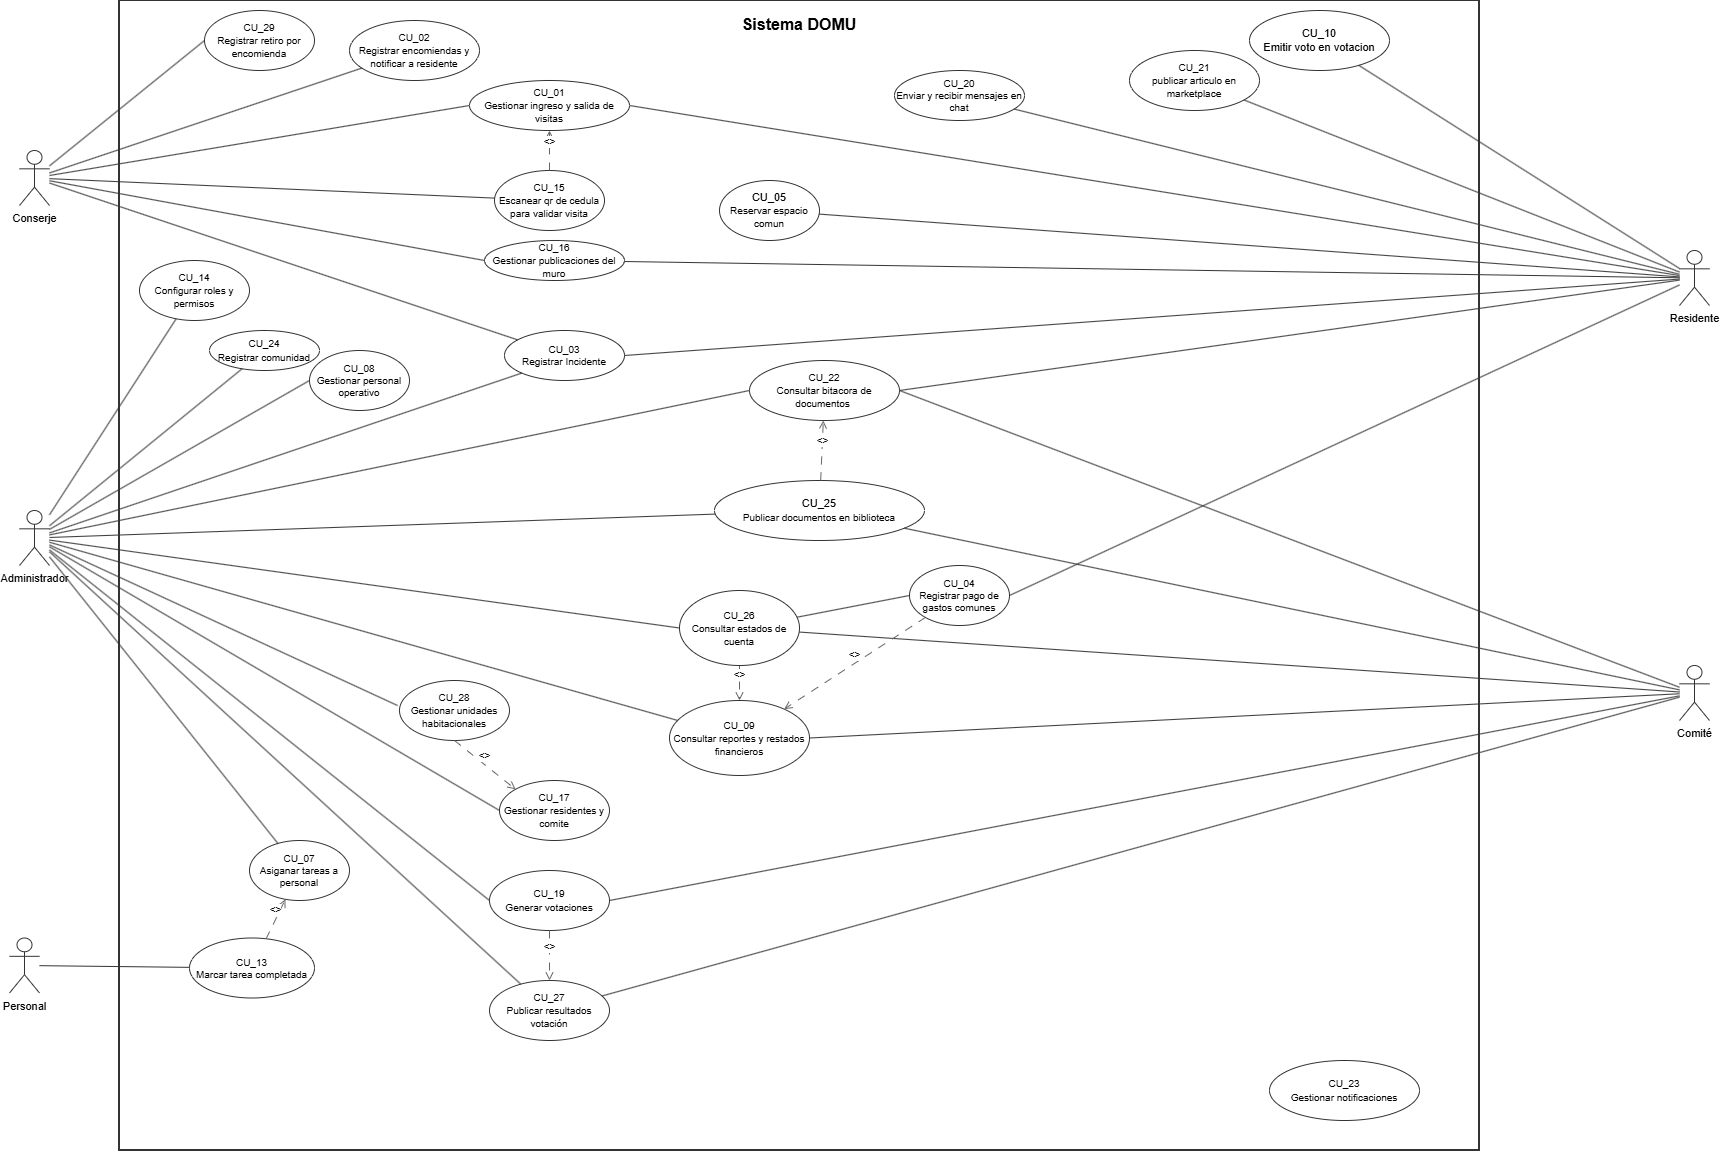
\includegraphics[width=0.98\textwidth]{images/ActoresCU-Diagrama General de Casos de Uso.drawio.png}
  \caption{Diagrama general de los principales casos de uso vigentes del sistema DOMU.}
  \label{fig:diagrama-cu}
\end{figure}

\subsection{Especificacion detallada de Casos de Uso}

% CU_01
\begin{table}[H]\centering
\begin{tabular}{|p{0.475\linewidth}|p{0.475\linewidth}|}\hline
\cutop{CU\_01}{Gestionar ingreso y salida de visitas}
\cusec{Precondiciones}{Residente y/o conserje autenticado segun el punto del flujo; existe una unidad de destino en la comunidad.}
\cusec{Includes}{---}
\cusec{Extends}{CU\_15 Escanear QR de cedula para validar visita, cuando el ingreso se apoya en la lectura del documento de identidad.}
\cuheader{Residente / Conserje}{Sistema}
1) El residente pre-autoriza la visita o el conserje inicia un registro manual al momento del arribo. & 2) Muestra los datos de la visita autorizada o despliega el formulario de registro. \\\hline
3) El conserje identifica a la visita y selecciona la unidad de destino. & 4) Valida datos del visitante, unidad asociada y vigencia del acceso. \\\hline
5) El conserje registra el ingreso o la salida. & 6) Guarda el movimiento y notifica al residente cuando corresponde. \\\hline
\multicolumn{2}{|l|}{\textbf{Flujo de eventos alternativos}}\\\hline
4a. La identificacion es invalida o la unidad no existe. & 4b. Rechaza el registro y solicita corregir los datos. \\\hline
4c. No existe autorizacion previa. & 4d. Permite continuar con registro manual segun validacion de conserjeria. \\\hline
\cusec{Post condiciones}{La visita queda registrada en el sistema con trazabilidad de ingreso y/o salida.}
\end{tabular}
\caption{CU\_01 --- Gestionar ingreso y salida de visitas}
\label{tab:cu01}
\end{table}

% CU_02
\begin{table}[H]\centering
\begin{tabular}{|p{0.475\linewidth}|p{0.475\linewidth}|}\hline
\cutop{CU\_02}{Registrar encomiendas y notificar a residentes}
\cusec{Precondiciones}{Conserje autenticado; la encomienda fue recibida en conserjeria y existe una unidad de destino.}
\cusec{Includes}{---}
\cusec{Extends}{---}
\cuheader{Conserje}{Sistema}
1) Accede al modulo de encomiendas y selecciona registrar recepcion. & 2) Muestra formulario de nueva encomienda. \\\hline
3) Ingresa remitente, descripcion, unidad y evidencia opcional. & 4) Valida los datos y crea la encomienda asociada a la unidad. \\\hline
5) Confirma el registro. & 6) Guarda la encomienda con estado ``Por retirar'' y notifica al residente. \\\hline
\multicolumn{2}{|l|}{\textbf{Flujo de eventos alternativos}}\\\hline
3a. La unidad indicada no existe. & 3b. Muestra error y solicita seleccionar una unidad valida. \\\hline
3c. La evidencia adjunta no es valida. & 3d. Permite continuar sin archivo o solicitar una nueva carga. \\\hline
\cusec{Post condiciones}{La encomienda queda registrada y disponible para seguimiento por conserjeria, administracion y residente.}
\end{tabular}
\caption{CU\_02 --- Registrar encomiendas y notificar a residentes}
\label{tab:cu02}
\end{table}

% CU_03
\begin{table}[H]\centering
\begin{tabular}{|p{0.475\linewidth}|p{0.475\linewidth}|}\hline
\cutop{CU\_03}{Registrar incidente}
\cusec{Precondiciones}{Residente, conserje o administrador autenticado; modulo de incidentes habilitado.}
\cusec{Includes}{---}
\cusec{Extends}{---}
\cuheader{Residente / Conserje / Administrador}{Sistema}
1) Accede al modulo de incidentes. & 2) Muestra el formulario de registro. \\\hline
3) Ingresa categoria, descripcion y antecedentes del incidente. & 4) Valida la informacion minima y permite adjuntar evidencia opcional. \\\hline
5) Confirma el reporte. & 6) Registra el incidente y lo deja disponible para seguimiento por administracion. \\\hline
\multicolumn{2}{|l|}{\textbf{Flujo de eventos alternativos}}\\\hline
3a. Falta informacion obligatoria. & 3b. Indica los campos faltantes y no permite registrar. \\\hline
4a. La evidencia adjunta no cumple formato o tamano. & 4b. Rechaza el archivo y mantiene el formulario para correccion. \\\hline
\cusec{Post condiciones}{Incidente registrado correctamente en el sistema.}
\end{tabular}
\caption{CU\_03 --- Registrar incidente}
\label{tab:cu03}
\end{table}

% CU_04
\begin{table}[H]\centering
\begin{tabular}{|p{0.475\linewidth}|p{0.475\linewidth}|}\hline
\cutop{CU\_04}{Registrar pago de gastos comunes}
\cusec{Precondiciones}{Residente autenticado; existe al menos un periodo pendiente de pago.}
\cusec{Includes}{CU\_09 Consultar reportes y estados financieros.}
\cusec{Extends}{---}
\cuheader{Residente / Administrador}{Sistema}
1) El residente selecciona el periodo pendiente que desea pagar. & 2) Muestra el detalle del estado de cuenta, cargos y saldo pendiente. \\\hline
3) El residente adjunta el comprobante de transferencia y confirma el envio. & 4) Valida el archivo y registra el pago con estado ``Pendiente de validacion''. \\\hline
5) El administrador revisa el comprobante asociado al periodo. & 6) Aprueba manualmente el pago y cambia el estado a ``Pagado'', o lo observa para una nueva carga. \\\hline
\multicolumn{2}{|l|}{\textbf{Flujo de eventos alternativos}}\\\hline
3a. El archivo no cumple con el formato esperado. & 3b. Rechaza la carga y solicita un nuevo comprobante. \\\hline
5a. El comprobante no es valido o no coincide con el cargo. & 5b. Mantiene el estado pendiente de validacion y registra observacion administrativa. \\\hline
\cusec{Post condiciones}{El comprobante queda asociado al periodo y el pago queda pendiente o validado segun la revision administrativa.}
\end{tabular}
\caption{CU\_04 --- Registrar pago de gastos comunes}
\label{tab:cu04}
\end{table}

% CU_05
\begin{table}[H]\centering
\begin{tabular}{|p{0.475\linewidth}|p{0.475\linewidth}|}\hline
\cutop{CU\_05}{Reservar espacio comun}
\cusec{Precondiciones}{Residente autenticado; existen espacios comunes y franjas horarias configuradas.}
\cusec{Includes}{---}
\cusec{Extends}{---}
\cuheader{Residente}{Sistema}
1) Selecciona el espacio comun y la fecha deseada. & 2) Muestra disponibilidad por bloque horario. \\\hline
3) Elige un horario y confirma la reserva. & 4) Valida reglas de disponibilidad, aforo y restricciones por mora. \\\hline
5) Finaliza la solicitud. & 6) Registra la reserva y actualiza el calendario del espacio comun. \\\hline
\multicolumn{2}{|l|}{\textbf{Flujo de eventos alternativos}}\\\hline
4a. El horario ya no esta disponible. & 4b. Informa el conflicto y ofrece horarios alternativos. \\\hline
4c. El residente tiene bloqueo por mora. & 4d. Deniega la reserva e informa el motivo. \\\hline
\cusec{Post condiciones}{El espacio queda reservado para la fecha y bloque seleccionado.}
\end{tabular}
\caption{CU\_05 --- Reservar espacio comun}
\label{tab:cu05}
\end{table}

% CU_07
\begin{table}[H]\centering
\begin{tabular}{|p{0.475\linewidth}|p{0.475\linewidth}|}\hline
\cutop{CU\_07}{Asignar tareas a personal}
\cusec{Precondiciones}{Administrador autenticado; existe personal operativo activo en el sistema.}
\cusec{Includes}{---}
\cusec{Extends}{CU\_13 Marcar tarea completada.}
\cuheader{Administrador}{Sistema}
1) Ingresa al modulo de tareas y crea una nueva tarea. & 2) Muestra formulario de definicion y asignacion. \\\hline
3) Ingresa descripcion, prioridad, fecha limite y responsable. & 4) Valida la informacion y registra la tarea. \\\hline
5) Confirma la asignacion. & 6) Notifica al personal responsable y deja la tarea en estado ``Asignada''. \\\hline
\multicolumn{2}{|l|}{\textbf{Flujo de eventos alternativos}}\\\hline
3a. Falta descripcion o responsable. & 3b. Solicita completar los campos obligatorios. \\\hline
\cusec{Post condiciones}{La tarea queda asignada y visible para el personal operativo correspondiente.}
\end{tabular}
\caption{CU\_07 --- Asignar tareas a personal}
\label{tab:cu07}
\end{table}

% CU_08
\begin{table}[H]\centering
\begin{tabular}{|p{0.475\linewidth}|p{0.475\linewidth}|}\hline
\cutop{CU\_08}{Gestionar personal operativo}
\cusec{Precondiciones}{Administrador autenticado; comunidad activa.}
\cusec{Includes}{---}
\cusec{Extends}{---}
\cuheader{Administrador}{Sistema}
1) Accede al modulo de personal operativo. & 2) Muestra listado del personal registrado y acciones disponibles. \\\hline
3) Crea, edita o elimina un registro de personal. & 4) Valida la informacion y actualiza el registro correspondiente. \\\hline
5) Asigna el rol o tipo de personal (conserje, aseo, mantencion u otro). & 6) Guarda los cambios y actualiza la disponibilidad del personal en el sistema. \\\hline
\multicolumn{2}{|l|}{\textbf{Flujo de eventos alternativos}}\\\hline
3a. El correo o identificador ya existe. & 3b. Informa el conflicto y solicita correccion. \\\hline
3c. Se intenta eliminar personal con dependencias activas. & 3d. Solicita resolver las dependencias antes de completar la operacion. \\\hline
\cusec{Post condiciones}{El personal operativo queda actualizado segun las acciones realizadas por administracion.}
\end{tabular}
\caption{CU\_08 --- Gestionar personal operativo}
\label{tab:cu08}
\end{table}

% CU_09
\begin{table}[H]\centering
\begin{tabular}{|p{0.475\linewidth}|p{0.475\linewidth}|}\hline
\cutop{CU\_09}{Consultar reportes y estados financieros}
\cusec{Precondiciones}{Administrador o Comite autenticado; existen periodos y cargos registrados en el sistema.}
\cusec{Includes}{---}
\cusec{Extends}{---}
\cuheader{Administrador / Comite}{Sistema}
1) Ingresa al modulo financiero o panel de reportes. & 2) Lista periodos, estados de cuenta, pagos y documentos disponibles. \\\hline
3) Selecciona el periodo, unidad o vista financiera a revisar. & 4) Muestra cargos, pagos, saldo, resumen del periodo y estadisticas disponibles. \\\hline
5) Solicita descargar o visualizar el documento asociado. & 6) Genera o entrega el archivo disponible y registra la consulta para trazabilidad. \\\hline
\multicolumn{2}{|l|}{\textbf{Flujo de eventos alternativos}}\\\hline
2a. No existen periodos publicados para el filtro seleccionado. & 2b. Informa que no hay informacion disponible para el rango solicitado. \\\hline
5a. El documento no esta generado. & 5b. Muestra el detalle en pantalla y registra la falta del archivo exportable. \\\hline
\cusec{Post condiciones}{La informacion financiera queda consultada y, cuando existe soporte documental, puede descargarse desde el sistema.}
\end{tabular}
\caption{CU\_09 --- Consultar reportes y estados financieros}
\label{tab:cu09}
\end{table}

% CU_10
\begin{table}[H]\centering
\begin{tabular}{|p{0.475\linewidth}|p{0.475\linewidth}|}\hline
\cutop{CU\_10}{Emitir voto en votacion comunitaria}
\cusec{Precondiciones}{Residente autenticado; existe una votacion abierta y habilitada para su participacion.}
\cusec{Includes}{---}
\cusec{Extends}{---}
\cuheader{Residente}{Sistema}
1) Ingresa al modulo de votaciones. & 2) Lista las votaciones abiertas y sus antecedentes. \\\hline
3) Selecciona una votacion y revisa las opciones disponibles. & 4) Valida habilitacion, registra el voto y actualiza el estado de participacion. \\\hline
5) Confirma su opcion. & 6) Guarda el voto y deja trazabilidad del sufragio emitido. \\\hline
\multicolumn{2}{|l|}{\textbf{Flujo de eventos alternativos}}\\\hline
4a. El residente ya voto. & 4b. Informa que la votacion ya fue respondida y bloquea un nuevo envio. \\\hline
4c. La votacion se encuentra cerrada. & 4d. Muestra solo los resultados o el estado historico, sin permitir votar. \\\hline
\cusec{Post condiciones}{El voto queda registrado correctamente para la votacion seleccionada.}
\end{tabular}
\caption{CU\_10 --- Emitir voto en votacion comunitaria}
\label{tab:cu10}
\end{table}

% CU_13
\begin{table}[H]\centering
\begin{tabular}{|p{0.475\linewidth}|p{0.475\linewidth}|}\hline
\cutop{CU\_13}{Marcar tarea completada}
\cusec{Precondiciones}{Personal operativo autenticado; existe una tarea asignada en estado pendiente o en progreso.}
\cusec{Includes}{---}
\cusec{Extends}{---}
\cuheader{Personal operativo}{Sistema}
1) Accede a la tarea asignada. & 2) Muestra detalle, prioridad y fecha comprometida. \\\hline
3) Marca la tarea como completada y adjunta evidencia si corresponde. & 4) Actualiza el estado de la tarea y registra fecha de cierre. \\\hline
5) Confirma el cierre. & 6) Notifica a administracion que la tarea fue completada. \\\hline
\multicolumn{2}{|l|}{\textbf{Flujo de eventos alternativos}}\\\hline
3a. La evidencia no cumple con el formato permitido. & 3b. Solicita una nueva carga o permite cerrar sin adjunto. \\\hline
\cusec{Post condiciones}{La tarea queda cerrada o avanzada con respaldo operacional en el sistema.}
\end{tabular}
\caption{CU\_13 --- Marcar tarea completada}
\label{tab:cu13}
\end{table}

% CU_14
\begin{table}[H]\centering
\begin{tabular}{|p{0.475\linewidth}|p{0.475\linewidth}|}\hline
\cutop{CU\_14}{Configurar roles y permisos}
\cusec{Precondiciones}{Administrador autenticado con privilegios de seguridad.}
\cusec{Includes}{---}
\cusec{Extends}{---}
\cuheader{Administrador}{Sistema}
1) Accede a la configuracion de roles y permisos. & 2) Muestra roles disponibles y permisos asociados por modulo. \\\hline
3) Crea o ajusta permisos de un rol existente. & 4) Valida consistencia de la configuracion y guarda la politica de acceso. \\\hline
5) Asigna el rol correspondiente a un usuario. & 6) Actualiza permisos efectivos y deja registro de auditoria. \\\hline
\multicolumn{2}{|l|}{\textbf{Flujo de eventos alternativos}}\\\hline
3a. La configuracion genera conflicto de permisos. & 3b. Informa la colision y no aplica los cambios hasta su correccion. \\\hline
\cusec{Post condiciones}{La configuracion de acceso queda actualizada y trazada.}
\end{tabular}
\caption{CU\_14 --- Configurar roles y permisos}
\label{tab:cu14}
\end{table}

% CU_15
\begin{table}[H]\centering
\begin{tabular}{|p{0.475\linewidth}|p{0.475\linewidth}|}\hline
\cutop{CU\_15}{Escanear QR de cedula para validar visita}
\cusec{Precondiciones}{Conserje autenticado; la visita presenta una cedula de identidad chilena con QR legible; el lector QR se encuentra operativo.}
\cusec{Includes}{---}
\cusec{Extends}{CU\_01 Gestionar ingreso y salida de visitas.}
\cuheader{Conserje}{Sistema}
1) Escanea el QR de la cedula del visitante. & 2) Extrae RUN y datos de identificacion disponibles desde el documento. \\\hline
3) Solicita la validacion del documento. & 4) Busca coincidencias con registros previos y autocompleta el formulario de visita. \\\hline
5) Confirma el uso de los datos recuperados. & 6) Deja la identificacion lista para continuar el flujo de ingreso. \\\hline
\multicolumn{2}{|l|}{\textbf{Flujo de eventos alternativos}}\\\hline
2a. El QR no puede leerse o esta incompleto. & 2b. Informa el error y permite continuar con ingreso manual de datos. \\\hline
\cusec{Post condiciones}{La identidad del visitante queda validada o precargada para el registro de la visita.}
\end{tabular}
\caption{CU\_15 --- Escanear QR de cedula para validar visita}
\label{tab:cu15}
\end{table}

% CU_16
\begin{table}[H]\centering
\begin{tabular}{|p{0.475\linewidth}|p{0.475\linewidth}|}\hline
\cutop{CU\_16}{Gestionar publicaciones del muro comunitario}
\cusec{Precondiciones}{Administrador o residente autenticado; modulo de publicaciones habilitado.}
\cusec{Includes}{---}
\cusec{Extends}{---}
\cuheader{Administrador / Residente}{Sistema}
1) El administrador accede al muro para publicar, o el residente ingresa para revisar publicaciones vigentes. & 2) Muestra el listado del muro y, para administracion, el formulario de nueva publicacion. \\\hline
3) El administrador ingresa categoria, titulo y contenido del aviso. & 4) Valida los datos y publica el contenido en el muro de la comunidad. \\\hline
5) El residente consulta, filtra o abre una publicacion. & 6) Despliega el contenido y registra la visualizacion en el contexto de la comunidad. \\\hline
\multicolumn{2}{|l|}{\textbf{Flujo de eventos alternativos}}\\\hline
3a. Faltan campos obligatorios de la publicacion. & 3b. Informa el error y mantiene el formulario para correccion. \\\hline
5a. No existen publicaciones vigentes. & 5b. Muestra estado vacio del muro comunitario. \\\hline
\cusec{Post condiciones}{Las publicaciones quedan visibles para los residentes y disponibles para consulta posterior.}
\end{tabular}
\caption{CU\_16 --- Gestionar publicaciones del muro comunitario}
\label{tab:cu16}
\end{table}

% CU_17
\begin{table}[H]\centering
\begin{tabular}{|p{0.475\linewidth}|p{0.475\linewidth}|}\hline
\cutop{CU\_17}{Gestionar residentes y comite}
\cusec{Precondiciones}{Administrador autenticado; comunidad activa y modulos administrativos disponibles.}
\cusec{Includes}{CU\_28 Gestionar unidades habitacionales, cuando se requiere asignar o reasignar una unidad.}
\cusec{Extends}{---}
\cuheader{Administrador}{Sistema}
1) Accede al modulo de usuarios de la comunidad. & 2) Muestra listado de residentes y miembros del comite registrados. \\\hline
3) Crea o edita la ficha del usuario comunitario. & 4) Valida datos personales, rol y estado del registro. \\\hline
5) Asigna rol de residente o comite y vincula la unidad cuando corresponde. & 6) Guarda los cambios y actualiza la informacion visible para la comunidad. \\\hline
\multicolumn{2}{|l|}{\textbf{Flujo de eventos alternativos}}\\\hline
3a. El correo o documento ya existe en la comunidad. & 3b. Informa el conflicto y no permite duplicar el registro. \\\hline
5a. La unidad seleccionada no esta disponible. & 5b. Solicita escoger otra unidad o revisar la asociacion actual. \\\hline
\cusec{Post condiciones}{La informacion de residentes y comite queda actualizada y vinculada a la comunidad activa.}
\end{tabular}
\caption{CU\_17 --- Gestionar residentes y comite}
\label{tab:cu17}
\end{table}

% CU_19
\begin{table}[H]\centering
\begin{tabular}{|p{0.475\linewidth}|p{0.475\linewidth}|}\hline
\cutop{CU\_19}{Gestionar votaciones comunitarias}
\cusec{Precondiciones}{Administrador o Comite autenticado; modulo de votaciones habilitado.}
\cusec{Includes}{---}
\cusec{Extends}{CU\_27 Publicar resultados de votacion, una vez cerrada la votacion.}
\cuheader{Administrador / Comite}{Sistema}
1) Ingresa al modulo de votaciones y selecciona crear o administrar una votacion. & 2) Muestra historial, estado actual y formulario de configuracion. \\\hline
3) Define titulo, descripcion, opciones y fecha de cierre. & 4) Valida el formulario y registra la votacion en estado abierta. \\\hline
5) Publica o cierra la votacion segun corresponda. & 6) Notifica a la comunidad y actualiza el historial del proceso. \\\hline
\multicolumn{2}{|l|}{\textbf{Flujo de eventos alternativos}}\\\hline
3a. Hay menos de dos opciones o la fecha no es valida. & 3b. Solicita corregir la configuracion antes de publicar. \\\hline
\cusec{Post condiciones}{La votacion queda creada, administrada o cerrada segun la accion ejecutada.}
\end{tabular}
\caption{CU\_19 --- Gestionar votaciones comunitarias}
\label{tab:cu19}
\end{table}

% CU_20
\begin{table}[H]\centering
\begin{tabular}{|p{0.475\linewidth}|p{0.475\linewidth}|}\hline
\cutop{CU\_20}{Enviar y recibir mensajes en chat}
\cusec{Precondiciones}{Residente autenticado; canal de chat habilitado en la comunidad.}
\cusec{Includes}{---}
\cusec{Extends}{---}
\cuheader{Residente}{Sistema}
1) Accede al modulo de chat y selecciona una conversacion o inicia una nueva. & 2) Muestra salas disponibles y el historial del chat seleccionado. \\\hline
3) Escribe y envia un mensaje. & 4) Transmite el mensaje en tiempo real y lo almacena en el historial. \\\hline
5) Recibe nuevas respuestas. & 6) Actualiza el estado de lectura y notifica actividad cuando corresponde. \\\hline
\multicolumn{2}{|l|}{\textbf{Flujo de eventos alternativos}}\\\hline
3a. La conversacion no esta disponible o fue ocultada. & 3b. Informa el estado y bloquea el envio hasta recuperar acceso. \\\hline
\cusec{Post condiciones}{La conversacion queda actualizada con los mensajes intercambiados.}
\end{tabular}
\caption{CU\_20 --- Enviar y recibir mensajes en chat}
\label{tab:cu20}
\end{table}

% CU_21
\begin{table}[H]\centering
\begin{tabular}{|p{0.475\linewidth}|p{0.475\linewidth}|}\hline
\cutop{CU\_21}{Publicar articulo en marketplace}
\cusec{Precondiciones}{Residente autenticado; marketplace comunitario habilitado.}
\cusec{Includes}{---}
\cusec{Extends}{---}
\cuheader{Residente}{Sistema}
1) Accede al marketplace y selecciona crear publicacion. & 2) Muestra formulario de articulo y carga de imagenes. \\\hline
3) Ingresa titulo, descripcion, precio y fotos. & 4) Valida la informacion y almacena la publicacion. \\\hline
5) Publica, edita o elimina el articulo. & 6) Actualiza el listado comunitario y deja trazabilidad del anuncio. \\\hline
\multicolumn{2}{|l|}{\textbf{Flujo de eventos alternativos}}\\\hline
3a. Las imagenes no cumplen el formato permitido. & 3b. Rechaza los archivos y solicita una nueva carga. \\\hline
\cusec{Post condiciones}{El articulo queda disponible en el marketplace o actualizado segun la accion realizada.}
\end{tabular}
\caption{CU\_21 --- Publicar articulo en marketplace}
\label{tab:cu21}
\end{table}

% CU_22
\begin{table}[H]\centering
\begin{tabular}{|p{0.475\linewidth}|p{0.475\linewidth}|}\hline
\cutop{CU\_22}{Consultar biblioteca de documentos}
\cusec{Precondiciones}{Administrador, residente o Comite autenticado; existen documentos publicados en la biblioteca.}
\cusec{Includes}{---}
\cusec{Extends}{---}
\cuheader{Administrador / Residente / Comite}{Sistema}
1) Accede al modulo Biblioteca. & 2) Lista documentos disponibles por categoria y nombre. \\\hline
3) Filtra o selecciona un documento. & 4) Permite visualizarlo o descargarlo desde el repositorio documental. \\\hline
\multicolumn{2}{|l|}{\textbf{Flujo de eventos alternativos}}\\\hline
4a. El archivo no se encuentra disponible. & 4b. Informa el problema y mantiene el documento como no descargable. \\\hline
\cusec{Post condiciones}{El documento queda consultado o descargado por el actor correspondiente.}
\end{tabular}
\caption{CU\_22 --- Consultar biblioteca de documentos}
\label{tab:cu22}
\end{table}

% CU_23
\begin{table}[H]\centering
\begin{tabular}{|p{0.475\linewidth}|p{0.475\linewidth}|}\hline
\cutop{CU\_23}{Gestionar notificaciones}
\cusec{Precondiciones}{Usuario autenticado.}
\cusec{Includes}{---}
\cusec{Extends}{---}
\cuheader{Usuario}{Sistema}
1) Abre el centro de notificaciones. & 2) Muestra notificaciones ordenadas por fecha y tipo. \\\hline
3) Marca notificaciones como leidas o ajusta preferencias. & 4) Actualiza el estado de lectura y la configuracion asociada. \\\hline
\multicolumn{2}{|l|}{\textbf{Flujo de eventos alternativos}}\\\hline
2a. No existen notificaciones para el usuario. & 2b. Muestra estado vacio y mantiene accesibles las preferencias. \\\hline
\cusec{Post condiciones}{El estado de lectura y las preferencias de notificacion quedan actualizados.}
\end{tabular}
\caption{CU\_23 --- Gestionar notificaciones}
\label{tab:cu23}
\end{table}

% CU_24
\begin{table}[H]\centering
\begin{tabular}{|p{0.475\linewidth}|p{0.475\linewidth}|}\hline
\cutop{CU\_24}{Registrar y aprobar comunidad}
\cusec{Precondiciones}{Solicitante con informacion de la comunidad y documentacion de respaldo.}
\cusec{Includes}{---}
\cusec{Extends}{---}
\cuheader{Administrador}{Sistema}
1) Completa el formulario de solicitud de comunidad. & 2) Valida los datos y almacena los documentos adjuntos. \\\hline
3) Envia la solicitud. & 4) Notifica al flujo de aprobacion mediante correo electronico. \\\hline
5) El aprobador revisa y aprueba o rechaza la solicitud. & 6) Crea la comunidad y habilita la invitacion para el administrador responsable. \\\hline
\multicolumn{2}{|l|}{\textbf{Flujo de eventos alternativos}}\\\hline
5a. La solicitud es rechazada. & 5b. Registra el motivo e informa el resultado al solicitante. \\\hline
\cusec{Post condiciones}{La comunidad queda creada o rechazada con trazabilidad del proceso de aprobacion.}
\end{tabular}
\caption{CU\_24 --- Registrar y aprobar comunidad}
\label{tab:cu24}
\end{table}

% CU_25
\begin{table}[H]\centering
\begin{tabular}{|p{0.475\linewidth}|p{0.475\linewidth}|}\hline
\cutop{CU\_25}{Publicar documentos y actas en la biblioteca}
\cusec{Precondiciones}{Administrador o Comite autenticado; modulo Biblioteca habilitado.}
\cusec{Includes}{CU\_22 Consultar biblioteca de documentos.}
\cusec{Extends}{---}
\cuheader{Administrador / Comite}{Sistema}
1) Accede a la biblioteca y selecciona cargar documento. & 2) Muestra formulario de nombre, categoria y archivo. \\\hline
3) Adjunta el documento y define su categoria. & 4) Valida formato, metadatos y permisos de carga. \\\hline
5) Confirma la publicacion. & 6) Guarda el documento y lo deja disponible para consulta en la comunidad. \\\hline
\multicolumn{2}{|l|}{\textbf{Flujo de eventos alternativos}}\\\hline
4a. El archivo no es valido o supera el limite permitido. & 4b. Rechaza la carga y solicita un nuevo archivo. \\\hline
4c. El Comite intenta usar una categoria distinta de ``actas''. & 4d. Restringe la categoria y solicita ajustarla a ``actas''. \\\hline
\cusec{Post condiciones}{El documento queda publicado en la biblioteca documental de la comunidad.}
\end{tabular}
\caption{CU\_25 --- Publicar documentos y actas en la biblioteca}
\label{tab:cu25}
\end{table}

% CU_26
\begin{table}[H]\centering
\begin{tabular}{|p{0.475\linewidth}|p{0.475\linewidth}|}\hline
\cutop{CU\_26}{Consultar estados de cuenta para fiscalizacion}
\cusec{Precondiciones}{Comite o administrador autenticado; existen periodos financieros publicados para consulta.}
\cusec{Includes}{CU\_09 Consultar reportes y estados financieros.}
\cusec{Extends}{---}
\cuheader{Comite / Administrador}{Sistema}
1) Ingresa al modulo financiero en modo consulta. & 2) Lista periodos y estados de cuenta disponibles. \\\hline
3) Selecciona el periodo que desea fiscalizar. & 4) Muestra detalle de cargos, pagos, saldo y documentos asociados. \\\hline
5) Consulta o descarga el respaldo disponible. & 6) Registra la accion para fines de trazabilidad y fiscalizacion. \\\hline
\multicolumn{2}{|l|}{\textbf{Flujo de eventos alternativos}}\\\hline
2a. El periodo aun no fue publicado. & 2b. Informa indisponibilidad del estado de cuenta solicitado. \\\hline
\cusec{Post condiciones}{El estado de cuenta queda consultado sin modificar la informacion financiera del sistema.}
\end{tabular}
\caption{CU\_26 --- Consultar estados de cuenta para fiscalizacion}
\label{tab:cu26}
\end{table}

% CU_27
\begin{table}[H]\centering
\begin{tabular}{|p{0.475\linewidth}|p{0.475\linewidth}|}\hline
\cutop{CU\_27}{Publicar resultados de votacion}
\cusec{Precondiciones}{Administrador o Comite autenticado; existe una votacion cerrada con resultados consolidados.}
\cusec{Includes}{---}
\cusec{Extends}{CU\_19 Gestionar votaciones comunitarias.}
\cuheader{Administrador / Comite}{Sistema}
1) Selecciona una votacion cerrada. & 2) Muestra resultados consolidados, total de votos y estado del proceso. \\\hline
3) Confirma la publicacion de resultados. & 4) Deja disponible el resultado en el historial y permite su descarga o consulta. \\\hline
5) Comunica el cierre a la comunidad. & 6) Registra la publicacion y notifica el resultado cuando corresponde. \\\hline
\multicolumn{2}{|l|}{\textbf{Flujo de eventos alternativos}}\\\hline
2a. La votacion aun esta abierta. & 2b. Impide la publicacion y exige cerrar primero el proceso. \\\hline
\cusec{Post condiciones}{Los resultados quedan publicados y disponibles para consulta historica.}
\end{tabular}
\caption{CU\_27 --- Publicar resultados de votacion}
\label{tab:cu27}
\end{table}

% CU_28
\begin{table}[H]\centering
\begin{tabular}{|p{0.475\linewidth}|p{0.475\linewidth}|}\hline
\cutop{CU\_28}{Gestionar unidades habitacionales}
\cusec{Precondiciones}{Administrador autenticado; comunidad activa.}
\cusec{Includes}{---}
\cusec{Extends}{---}
\cuheader{Administrador}{Sistema}
1) Accede al modulo de unidades habitacionales. & 2) Muestra listado de unidades y opciones de creacion o edicion. \\\hline
3) Crea, edita o elimina una unidad. & 4) Valida numero, torre, piso y metadatos asociados a la unidad. \\\hline
5) Asocia o desvincula residentes cuando corresponde. & 6) Guarda los cambios y actualiza la estructura habitacional de la comunidad. \\\hline
\multicolumn{2}{|l|}{\textbf{Flujo de eventos alternativos}}\\\hline
3a. Se intenta eliminar una unidad con residentes asociados. & 3b. Impide la eliminacion y solicita desvincular primero a los residentes. \\\hline
\cusec{Post condiciones}{Las unidades habitacionales quedan actualizadas y disponibles para operacion administrativa.}
\end{tabular}
\caption{CU\_28 --- Gestionar unidades habitacionales}
\label{tab:cu28}
\end{table}

% CU_29
\begin{table}[H]\centering
\begin{tabular}{|p{0.475\linewidth}|p{0.475\linewidth}|}\hline
\cutop{CU\_29}{Registrar retiro de encomienda}
\cusec{Precondiciones}{Conserje autenticado; existe una encomienda en estado ``Por retirar''.}
\cusec{Includes}{---}
\cusec{Extends}{---}
\cuheader{Conserje}{Sistema}
1) Busca la encomienda pendiente de retiro. & 2) Muestra el detalle de la encomienda y la unidad asociada. \\\hline
3) Verifica al residente o persona autorizada. & 4) Valida que la encomienda siga disponible para entrega. \\\hline
5) Marca la encomienda como retirada. & 6) Registra fecha y hora del retiro y actualiza el estado a ``Retirada''. \\\hline
\multicolumn{2}{|l|}{\textbf{Flujo de eventos alternativos}}\\\hline
4a. La encomienda ya fue retirada. & 4b. Informa el estado actual y bloquea un nuevo cierre. \\\hline
4c. No es posible validar al receptor. & 4d. Mantiene la encomienda en estado ``Por retirar''. \\\hline
\cusec{Post condiciones}{La encomienda queda entregada y con trazabilidad del retiro en el sistema.}
\end{tabular}
\caption{CU\_29 --- Registrar retiro de encomienda}
\label{tab:cu29}
\end{table}

% \subsection{Diagramas de casos de uso por modulo}

% A continuacion se presentan diagramas resumidos por modulo funcional. Se mantienen como apoyo visual del analisis vigente y excluyen los casos de uso diferidos al Anexo~\ref{anexo:casos-restantes}.

% \begin{figure}[H]
%   \centering
%   \fbox{\parbox{0.85\textwidth}{\centering\vspace{3.2cm}
%   \textit{Modulo Visitas y Acceso: CU\_01 y CU\_15.}\\
%   \textit{Actores principales: Residente y Conserje.}
%   \vspace{3.2cm}}}
%   \caption{Diagrama de casos de uso --- Modulo Visitas y Acceso.}
%   \label{fig:cu-modulo-visitas}
% \end{figure}

% \begin{figure}[H]
%   \centering
%   \fbox{\parbox{0.85\textwidth}{\centering\vspace{3.2cm}
%   \textit{Modulo Encomiendas e Incidentes: CU\_02, CU\_03 y CU\_29.}\\
%   \textit{Actores principales: Conserje, Residente y Administrador.}
%   \vspace{3.2cm}}}
%   \caption{Diagrama de casos de uso --- Modulo Encomiendas e Incidentes.}
%   \label{fig:cu-modulo-encomiendas}
% \end{figure}

% \begin{figure}[H]
%   \centering
%   \fbox{\parbox{0.85\textwidth}{\centering\vspace{3.2cm}
%   \textit{Modulo Financiero: CU\_04, CU\_09 y CU\_26.}\\
%   \textit{Actores principales: Residente, Administrador y Comite.}
%   \vspace{3.2cm}}}
%   \caption{Diagrama de casos de uso --- Modulo Financiero.}
%   \label{fig:cu-modulo-financiero}
% \end{figure}

% \begin{figure}[H]
%   \centering
%   \fbox{\parbox{0.85\textwidth}{\centering\vspace{3.2cm}
%   \textit{Modulo Comunidad: CU\_10, CU\_16, CU\_19, CU\_20, CU\_21, CU\_22, CU\_25 y CU\_27.}\\
%   \textit{Actores principales: Residente, Administrador y Comite.}
%   \vspace{3.2cm}}}
%   \caption{Diagrama de casos de uso --- Modulo Comunidad y Gobernanza.}
%   \label{fig:cu-modulo-comunidad}
% \end{figure}

% \begin{figure}[H]
%   \centering
%   \fbox{\parbox{0.85\textwidth}{\centering\vspace{3.2cm}
%   \textit{Modulo Administrativo: CU\_07, CU\_08, CU\_14, CU\_17, CU\_24 y CU\_28.}\\
%   \textit{Actores principales: Administrador y Personal operativo.}
%   \vspace{3.2cm}}}
%   \caption{Diagrama de casos de uso --- Modulo Administrativo.}
%   \label{fig:cu-modulo-admin}
% \end{figure}

\section{Matriz de trazabilidad RF--CU}

\begin{longtable}{|m{3cm}|m{12.5cm}|}
\hline
\textbf{RF} & \textbf{Casos de Uso relacionados} \\\hline
RF\_01 (Visitas) & CU\_01, CU\_15 \\\hline
RF\_02 (Notificaciones push) & CU\_01, CU\_02, CU\_03, CU\_04, CU\_07, CU\_13, CU\_19, CU\_23, CU\_29 \\\hline
RF\_03 (Pre-autorizacion de visitas) & CU\_01, CU\_15 \\\hline
RF\_04 (Encomiendas) & CU\_02, CU\_29 \\\hline
RF\_05 (Tareas del personal) & CU\_07, CU\_08, CU\_13 \\\hline
RF\_06 (Inicio/fin jornada) & Cobertura parcial en v1.0 mediante CU\_13; la marcacion de jornada queda diferida al anexo. \\\hline
RF\_07 (Estado de cuenta y pago) & CU\_04, CU\_09, CU\_26 \\\hline
RF\_08 (Morosidad/conciliacion) & Sin CU vigente en el cuerpo principal; vease Anexo~\ref{anexo:casos-restantes} (CU\_06). \\\hline
RF\_09 (Reservas) & CU\_05 \\\hline
RF\_10 (Votaciones) & CU\_10, CU\_19, CU\_27 \\\hline
RF\_11 (Comunicacion comunitaria) & CU\_16, CU\_20 \\\hline
RF\_12 (Tickets de reclamos) & CU\_03 \\\hline
RF\_13 (Gestion de votaciones por Administracion/Comite) & CU\_19, CU\_27 \\\hline
RF\_14 (Mantenimiento preventivo) & Sin CU vigente en el cuerpo principal; vease Anexo~\ref{anexo:casos-restantes} (CU\_11 y CU\_18). \\\hline
RF\_15 (Dashboards/KPI) & CU\_09 \\\hline
RF\_16 (RBAC y configuracion administrativa) & CU\_14, CU\_17, CU\_24, CU\_28 \\\hline
RF\_17 (Chat en tiempo real) & CU\_20 \\\hline
RF\_18 (Marketplace) & CU\_21 \\\hline
RF\_19 (Biblioteca documental) & CU\_22, CU\_25 \\\hline
RF\_20 (Notificaciones en tiempo real) & CU\_01, CU\_02, CU\_03, CU\_04, CU\_07, CU\_13, CU\_19, CU\_23, CU\_29 \\\hline
\caption{Matriz de trazabilidad RF--CU de la version vigente.}
\label{tab:traza-compacta}
\end{longtable}

\begin{landscape}
\scriptsize
\setlength{\tabcolsep}{2pt}
\renewcommand{\arraystretch}{1.1}
\begin{longtable}{|l|*{25}{c|}}
\hline
\textbf{RF \textbackslash\ CU} & \textbf{01} & \textbf{02} & \textbf{03} & \textbf{04} & \textbf{05} & \textbf{07} & \textbf{08} & \textbf{09} & \textbf{10} & \textbf{13} & \textbf{14} & \textbf{15} & \textbf{16} & \textbf{17} & \textbf{19} & \textbf{20} & \textbf{21} & \textbf{22} & \textbf{23} & \textbf{24} & \textbf{25} & \textbf{26} & \textbf{27} & \textbf{28} & \textbf{29}\\\hline
RF\_01 & X &  &  &  &  &  &  &  &  &  &  & X &  &  &  &  &  &  &  &  &  &  &  &  &  \\\hline
RF\_02 & X & X & X & X &  & X &  &  &  & X &  &  &  &  & X &  &  &  & X &  &  &  &  &  & X \\\hline
RF\_03 & X &  &  &  &  &  &  &  &  &  &  & X &  &  &  &  &  &  &  &  &  &  &  &  &  \\\hline
RF\_04 &  & X &  &  &  &  &  &  &  &  &  &  &  &  &  &  &  &  &  &  &  &  &  &  & X \\\hline
RF\_05 &  &  &  &  &  & X & X &  &  & X &  &  &  &  &  &  &  &  &  &  &  &  &  &  &  \\\hline
RF\_06 &  &  &  &  &  &  &  &  &  & X &  &  &  &  &  &  &  &  &  &  &  &  &  &  &  \\\hline
RF\_07 &  &  &  & X &  &  &  & X &  &  &  &  &  &  &  &  &  &  &  &  &  & X &  &  &  \\\hline
RF\_08 &  &  &  &  &  &  &  &  &  &  &  &  &  &  &  &  &  &  &  &  &  &  &  &  &  \\\hline
RF\_09 &  &  &  &  & X &  &  &  &  &  &  &  &  &  &  &  &  &  &  &  &  &  &  &  &  \\\hline
RF\_10 &  &  &  &  &  &  &  &  & X &  &  &  &  &  & X &  &  &  &  &  &  &  & X &  &  \\\hline
RF\_11 &  &  &  &  &  &  &  &  &  &  &  &  & X &  &  & X &  &  &  &  &  &  &  &  &  \\\hline
RF\_12 &  &  & X &  &  &  &  &  &  &  &  &  &  &  &  &  &  &  &  &  &  &  &  &  &  \\\hline
RF\_13 &  &  &  &  &  &  &  &  &  &  &  &  &  &  & X &  &  &  &  &  &  &  & X &  &  \\\hline
RF\_14 &  &  &  &  &  &  &  &  &  &  &  &  &  &  &  &  &  &  &  &  &  &  &  &  &  \\\hline
RF\_15 &  &  &  &  &  &  &  & X &  &  &  &  &  &  &  &  &  &  &  &  &  &  &  &  &  \\\hline
RF\_16 &  &  &  &  &  &  &  &  &  &  & X &  &  & X &  &  &  &  &  & X &  &  &  & X &  \\\hline
RF\_17 &  &  &  &  &  &  &  &  &  &  &  &  &  &  &  & X &  &  &  &  &  &  &  &  &  \\\hline
RF\_18 &  &  &  &  &  &  &  &  &  &  &  &  &  &  &  &  & X &  &  &  &  &  &  &  &  \\\hline
RF\_19 &  &  &  &  &  &  &  &  &  &  &  &  &  &  &  &  &  & X &  &  & X &  &  &  &  \\\hline
RF\_20 & X & X & X & X &  & X &  &  &  & X &  &  &  &  & X &  &  &  & X &  &  &  &  &  & X \\\hline
\caption{Matriz de trazabilidad RF--CU (version vigente).}
\label{tab:traza-grid}
\end{longtable}
\end{landscape}

% \section{Matriz de trazabilidad CU -- Vistas}

% La Tabla~\ref{tab:traza-cu-vistas} vincula cada caso de uso vigente con las vistas del frontend donde se materializa, completando la cadena de trazabilidad RF~$\rightarrow$~CU~$\rightarrow$~Pantalla. Las vistas se detallan en la Seccion~\ref{subsec:vistas-por-rol} del Capitulo~\ref{cap:diseno}.

% \begin{longtable}{|p{0.07\textwidth}|p{0.25\textwidth}|p{0.42\textwidth}|p{0.18\textwidth}|}
% \caption{Matriz de trazabilidad CU -- Vistas del frontend}\label{tab:traza-cu-vistas}\\
% \hline
% \textbf{CU} & \textbf{Nombre} & \textbf{Vista(s) Frontend} & \textbf{Rol principal} \\
% \hline
% \endfirsthead
% \hline
% \textbf{CU} & \textbf{Nombre} & \textbf{Vista(s) Frontend} & \textbf{Rol principal} \\
% \hline
% \endhead
% \hline
% \endfoot

% CU\_01 & Gestionar ingreso/salida de visitas & VisitRegistrationPanel, ResidentVisits & Residente, Conserje \\
% \hline
% CU\_02 & Registrar encomiendas & ConciergeParcels, AdminParcels, ResidentParcels & Conserje \\
% \hline
% CU\_03 & Registrar incidente & ResidentIncidents, AdminIncidentsBoard & Residente, Conserje, Administrador \\
% \hline
% CU\_04 & Registrar pago de gastos comunes & ResidentCartola, ResidentChargesDetail, ResidentPaymentFlow, AdminCommonExpenses & Residente, Administrador \\
% \hline
% CU\_05 & Reservar espacio comun & ResidentAmenities, AdminAmenities & Residente \\
% \hline
% CU\_07 & Asignar tareas & AdminTasks & Administrador \\
% \hline
% CU\_08 & Gestionar personal operativo & AdminStaff, AdminCreateUser & Administrador \\
% \hline
% CU\_09 & Consultar reportes y estados financieros & Dashboard, AdminCommonExpenses, AdminIncidentStats & Administrador, Comite \\
% \hline
% CU\_10 & Emitir voto & Votaciones & Residente \\
% \hline
% CU\_13 & Marcar tarea completada & StaffTasks, StaffPortal & Personal operativo \\
% \hline
% CU\_14 & Configurar roles y permisos & AdminCreateUser & Administrador \\
% \hline
% CU\_15 & Escanear QR de cedula & VisitRegistrationPanel & Conserje \\
% \hline
% CU\_16 & Gestionar publicaciones del muro comunitario & ResidentPublications & Administrador, Residente \\
% \hline
% CU\_17 & Gestionar residentes y comite & AdminResidents, AdminCreateUser & Administrador \\
% \hline
% CU\_19 & Gestionar votaciones comunitarias & Votaciones & Administrador, Comite \\
% \hline
% CU\_20 & Chat en tiempo real & ChatHub & Residente \\
% \hline
% CU\_21 & Publicar articulo en marketplace & ResidentMarketplace, ResidentMarketplaceCreate & Residente \\
% \hline
% CU\_22 & Consultar biblioteca documental & ResidentLibrary & Administrador, Residente, Comite \\
% \hline
% CU\_23 & Gestionar notificaciones & NotificationCenter, NotificationPreferences & Todos los roles \\
% \hline
% CU\_24 & Registrar/aprobar comunidad & CreateCommunityModal, CommunitySelector, AdminInviteRegister & Administrador \\
% \hline
% CU\_25 & Publicar documentos y actas & ResidentLibrary & Administrador, Comite \\
% \hline
% CU\_26 & Consultar estados de cuenta para fiscalizacion & AdminCommonExpenses, Dashboard & Comite, Administrador \\
% \hline
% CU\_27 & Publicar resultados de votacion & Votaciones & Administrador, Comite \\
% \hline
% CU\_28 & Gestionar unidades habitacionales & AdminHousingUnits & Administrador \\
% \hline
% CU\_29 & Registrar retiro de encomienda & ConciergeParcels, AdminParcels, ResidentParcels & Conserje \\

% \end{longtable}

\endgroup


\chapter{Diseño}
\label{cap:diseno}
Este capítulo abordará los servicios web necesarios para este proyecto, el modelo de datos, diagramas de entidad-relación y diseño de la plataforma DOMU. Se presenta el modelo de datos, la arquitectura del software y el diseño de las interfaces, que permiten visualizar cómo se implementarán los requerimientos funcionales y no funcionales definidos en el capítulo anterior.

% ---------------------------------------------
\section{Descripción de los Servicios Web}

La capa de servicios web de DOMU se implementa mediante una \textbf{API RESTful} expuesta a través del \textit{framework} Javalin~6, complementada con canales \textbf{WebSocket} para comunicación bidireccional en tiempo real. El backend agrupa la lógica en trece módulos funcionales, cada uno respaldado por sus respectivos \textit{Controllers}, \textit{Services} y \textit{Repositories}. Adicionalmente, el sistema integra servicios transversales de generación de documentos PDF (OpenPDF), almacenamiento en la nube (Box~API) y envío de correo electrónico (Jakarta~Mail).

La Tabla~\ref{tab:servicios-web} resume los módulos, el protocolo de comunicación que utilizan y una descripción sintética de su alcance funcional.

\begin{longtable}{|p{0.22\textwidth}|p{0.13\textwidth}|p{0.57\textwidth}|}
\caption{Módulos de servicios web del sistema DOMU}\label{tab:servicios-web}\\
\hline
\textbf{Módulo} & \textbf{Protocolo} & \textbf{Descripción} \\
\hline
\endfirsthead
\hline
\textbf{Módulo} & \textbf{Protocolo} & \textbf{Descripción} \\
\hline
\endhead
\hline
\endfoot

Autenticación y Autorización &
REST &
Registro con confirmación por correo, inicio de sesión con JWT, recuperación de contraseña mediante token temporal y cierre de sesión. \\
\hline

Gestión de Usuarios y Roles &
REST &
CRUD de usuarios, asignación dinámica de cinco roles (Administrador, Residente, Conserje, Funcionario, Proveedor) bajo el modelo RBAC; gestión de perfiles con avatar almacenado en Box. \\
\hline

Gestión de Comunidades &
REST / E-mail &
Registro de comunidades con aprobación por correo electrónico, invitación de administradores, soporte multi-comunidad y vinculación de usuarios a edificios. \\
\hline

Control de Accesos &
REST &
Registro de visitas, pre-autorización con código QR, check-in/check-out, gestión de contactos frecuentes y bitácora de ingresos. \\
\hline

Gestión de Encomiendas &
REST &
Recepción de paquetes, seguimiento de estados (recibido, notificado, retirado), evidencia fotográfica y notificación al residente. \\
\hline

Gestión Operativa &
REST &
Administración de personal y turnos, creación y asignación de tareas con evidencia fotográfica y seguimiento por estado. \\
\hline

Administración Financiera &
REST / PDF &
Períodos de gasto común, cargos por unidad, registro de pagos, generación de boletas y estados de cuenta en PDF (OpenPDF). \\
\hline

Incidentes y Tickets &
REST &
Reporte de incidencias por residentes, asignación a responsables, seguimiento por estado y prioridad. \\
\hline

Reservas de Áreas Comunes &
REST &
Definición de amenidades con franjas horarias, control de aforo, consulta de disponibilidad y gestión de reservas. \\
\hline

Votaciones &
REST &
Creación de procesos de votación, sufragio remoto, cierre automático y exportación de resultados. \\
\hline

Comunicación Comunitaria &
REST / WebSocket &
Foro con categorías e hilos, chat en tiempo real vía WebSocket (\texttt{/ws/chat}), marketplace de artículos entre vecinos y biblioteca de documentos comunitarios. \\
\hline

Notificaciones &
WebSocket &
Entrega de notificaciones en tiempo real mediante el canal \texttt{/ws/notifications}, con preferencias configurables por tipo de evento. \\
\hline

Gestión de Proveedores y Órdenes de Servicio &
REST &
CRUD de proveedores vinculados a la comunidad, creación y seguimiento de órdenes de servicio con flujo de aceptación/rechazo por parte del proveedor, y gestión de cotizaciones. \\

\end{longtable}

% ---------------------------------------------
\subsection{Especificación de Endpoints Principales}

A continuación se documentan los endpoints REST más representativos del sistema, agrupados por módulo funcional. La API completa cuenta con más de 130~endpoints; para la especificación exhaustiva e interactiva, se recomienda consultar Swagger~UI en la ruta \texttt{/swagger} del servidor.

% --- Endpoints: Autenticación ---
\begin{longtable}{|p{0.08\textwidth}|p{0.38\textwidth}|p{0.46\textwidth}|}
\caption{Endpoints --- Autenticación}\label{tab:ep-auth}\\
\hline
\textbf{Método} & \textbf{Ruta} & \textbf{Descripción} \\
\hline
\endfirsthead
\hline \textbf{Método} & \textbf{Ruta} & \textbf{Descripción} \\ \hline
\endhead
\hline \endfoot

POST & \texttt{/api/auth/register} & Registro de usuario con envío de correo de confirmación. \\
\hline
POST & \texttt{/api/auth/login} & Inicio de sesión; retorna token JWT. \\
\hline
GET & \texttt{/api/auth/confirm-email} & Confirma correo electrónico mediante token. \\
\hline
POST & \texttt{/api/auth/forgot-password} & Envía correo con enlace de recuperación de contraseña. \\
\hline
POST & \texttt{/api/auth/reset-password} & Restablece contraseña mediante token temporal. \\

\end{longtable}

% --- Endpoints: Usuarios ---
\begin{longtable}{|p{0.08\textwidth}|p{0.38\textwidth}|p{0.46\textwidth}|}
\caption{Endpoints --- Usuarios y Perfiles}\label{tab:ep-users}\\
\hline
\textbf{Método} & \textbf{Ruta} & \textbf{Descripción} \\
\hline
\endfirsthead
\hline \textbf{Método} & \textbf{Ruta} & \textbf{Descripción} \\ \hline
\endhead
\hline \endfoot

GET & \texttt{/api/users/profile} & Obtiene perfil del usuario autenticado. \\
\hline
PUT & \texttt{/api/users/profile} & Actualiza datos del perfil. \\
\hline
POST & \texttt{/api/users/avatar} & Sube o actualiza avatar (almacenado en Box). \\
\hline
GET & \texttt{/api/users} & Lista usuarios de la comunidad activa (filtro por rol). \\

\end{longtable}

% --- Endpoints: Comunidades ---
\begin{longtable}{|p{0.08\textwidth}|p{0.38\textwidth}|p{0.46\textwidth}|}
\caption{Endpoints --- Comunidades}\label{tab:ep-communities}\\
\hline
\textbf{Método} & \textbf{Ruta} & \textbf{Descripción} \\
\hline
\endfirsthead
\hline \textbf{Método} & \textbf{Ruta} & \textbf{Descripción} \\ \hline
\endhead
\hline \endfoot

POST & \texttt{/api/buildings} & Solicita registro de nueva comunidad. \\
\hline
POST & \texttt{/api/buildings/approve/\{token\}} & Aprueba solicitud de comunidad vía correo. \\
\hline
POST & \texttt{/api/buildings/reject/\{token\}} & Rechaza solicitud de comunidad. \\
\hline
GET & \texttt{/api/buildings} & Lista comunidades del usuario autenticado. \\
\hline
GET & \texttt{/api/buildings/\{id\}} & Obtiene detalle de una comunidad. \\

\end{longtable}

% --- Endpoints: Control de Accesos ---
\begin{longtable}{|p{0.08\textwidth}|p{0.38\textwidth}|p{0.46\textwidth}|}
\caption{Endpoints --- Control de Accesos}\label{tab:ep-access}\\
\hline
\textbf{Método} & \textbf{Ruta} & \textbf{Descripción} \\
\hline
\endfirsthead
\hline \textbf{Método} & \textbf{Ruta} & \textbf{Descripción} \\ \hline
\endhead
\hline \endfoot

POST & \texttt{/api/visits} & Registra nueva visita (ingreso). \\
\hline
POST & \texttt{/api/visits/qr-check} & Verifica código QR de visita pre-autorizada. \\
\hline
PUT & \texttt{/api/visits/\{id\}/checkout} & Registra salida de visita. \\
\hline
GET & \texttt{/api/visits} & Lista visitas de la comunidad (filtros por fecha y estado). \\
\hline
POST & \texttt{/api/visits/pre-authorize} & Pre-autoriza visita con generación de QR. \\
\hline
GET & \texttt{/api/visit-contacts} & Lista contactos frecuentes del residente. \\

\end{longtable}

% --- Endpoints: Encomiendas ---
\begin{longtable}{|p{0.08\textwidth}|p{0.38\textwidth}|p{0.46\textwidth}|}
\caption{Endpoints --- Encomiendas}\label{tab:ep-parcels}\\
\hline
\textbf{Método} & \textbf{Ruta} & \textbf{Descripción} \\
\hline
\endfirsthead
\hline \textbf{Método} & \textbf{Ruta} & \textbf{Descripción} \\ \hline
\endhead
\hline \endfoot

POST & \texttt{/api/parcels} & Registra nueva encomienda con evidencia fotográfica. \\
\hline
PUT & \texttt{/api/parcels/\{id\}/status} & Actualiza estado (notificado, retirado). \\
\hline
GET & \texttt{/api/parcels} & Lista encomiendas de la comunidad. \\
\hline
GET & \texttt{/api/parcels/\{id\}} & Detalle de una encomienda. \\

\end{longtable}

% --- Endpoints: Finanzas ---
\begin{longtable}{|p{0.08\textwidth}|p{0.38\textwidth}|p{0.46\textwidth}|}
\caption{Endpoints --- Administración Financiera}\label{tab:ep-finance}\\
\hline
\textbf{Método} & \textbf{Ruta} & \textbf{Descripción} \\
\hline
\endfirsthead
\hline \textbf{Método} & \textbf{Ruta} & \textbf{Descripción} \\ \hline
\endhead
\hline \endfoot

POST & \texttt{/api/common-expenses/periods} & Crea nuevo período de gasto común. \\
\hline
POST & \texttt{/api/common-expenses/charges} & Agrega cargos a un período por unidad. \\
\hline
POST & \texttt{/api/payments} & Registra pago de gasto común. \\
\hline
GET & \texttt{/api/common-expenses/statement/\{unitId\}} & Obtiene estado de cuenta de una unidad. \\
\hline
GET & \texttt{/api/common-expenses/statement/\{unitId\}/pdf} & Descarga estado de cuenta en PDF. \\
\hline
GET & \texttt{/api/payments} & Lista pagos registrados (filtros por período y unidad). \\

\end{longtable}

% --- Endpoints: Incidentes ---
\begin{longtable}{|p{0.08\textwidth}|p{0.38\textwidth}|p{0.46\textwidth}|}
\caption{Endpoints --- Incidentes y Tickets}\label{tab:ep-incidents}\\
\hline
\textbf{Método} & \textbf{Ruta} & \textbf{Descripción} \\
\hline
\endfirsthead
\hline \textbf{Método} & \textbf{Ruta} & \textbf{Descripción} \\ \hline
\endhead
\hline \endfoot

POST & \texttt{/api/incidents} & Crea nuevo ticket de incidencia. \\
\hline
PUT & \texttt{/api/incidents/\{id\}/status} & Actualiza estado del ticket. \\
\hline
GET & \texttt{/api/incidents} & Lista incidentes de la comunidad. \\
\hline
GET & \texttt{/api/incidents/stats} & Obtiene estadísticas de incidentes. \\

\end{longtable}

% --- Endpoints: Reservas ---
\begin{longtable}{|p{0.08\textwidth}|p{0.38\textwidth}|p{0.46\textwidth}|}
\caption{Endpoints --- Reservas de Áreas Comunes}\label{tab:ep-reservations}\\
\hline
\textbf{Método} & \textbf{Ruta} & \textbf{Descripción} \\
\hline
\endfirsthead
\hline \textbf{Método} & \textbf{Ruta} & \textbf{Descripción} \\ \hline
\endhead
\hline \endfoot

GET & \texttt{/api/amenities} & Lista áreas comunes de la comunidad. \\
\hline
GET & \texttt{/api/amenities/\{id\}/availability} & Consulta disponibilidad por fecha. \\
\hline
POST & \texttt{/api/reservations} & Crea reserva de área común. \\
\hline
DELETE & \texttt{/api/reservations/\{id\}} & Cancela reserva existente. \\

\end{longtable}

% --- Endpoints: Votaciones ---
\begin{longtable}{|p{0.08\textwidth}|p{0.38\textwidth}|p{0.46\textwidth}|}
\caption{Endpoints --- Votaciones}\label{tab:ep-polls}\\
\hline
\textbf{Método} & \textbf{Ruta} & \textbf{Descripción} \\
\hline
\endfirsthead
\hline \textbf{Método} & \textbf{Ruta} & \textbf{Descripción} \\ \hline
\endhead
\hline \endfoot

POST & \texttt{/api/polls} & Crea nueva votación con opciones y fecha de cierre. \\
\hline
POST & \texttt{/api/polls/\{id\}/vote} & Registra voto del usuario autenticado. \\
\hline
PUT & \texttt{/api/polls/\{id\}/close} & Cierra votación y consolida resultados. \\
\hline
GET & \texttt{/api/polls/\{id\}/results} & Obtiene resultados de la votación. \\

\end{longtable}

% --- Endpoints: Chat ---
\begin{longtable}{|p{0.08\textwidth}|p{0.38\textwidth}|p{0.46\textwidth}|}
\caption{Endpoints --- Chat}\label{tab:ep-chat}\\
\hline
\textbf{Método} & \textbf{Ruta} & \textbf{Descripción} \\
\hline
\endfirsthead
\hline \textbf{Método} & \textbf{Ruta} & \textbf{Descripción} \\ \hline
\endhead
\hline \endfoot

POST & \texttt{/api/chat/rooms} & Crea sala de chat o solicita conversación. \\
\hline
POST & \texttt{/api/chat/rooms/\{id\}/messages} & Envía mensaje a una sala (REST fallback). \\
\hline
GET & \texttt{/api/chat/rooms/\{id\}/messages} & Obtiene historial de mensajes. \\

\end{longtable}

% --- Endpoints: Notificaciones ---
\begin{longtable}{|p{0.08\textwidth}|p{0.38\textwidth}|p{0.46\textwidth}|}
\caption{Endpoints --- Notificaciones}\label{tab:ep-notifications}\\
\hline
\textbf{Método} & \textbf{Ruta} & \textbf{Descripción} \\
\hline
\endfirsthead
\hline \textbf{Método} & \textbf{Ruta} & \textbf{Descripción} \\ \hline
\endhead
\hline \endfoot

GET & \texttt{/api/notifications} & Lista notificaciones del usuario. \\
\hline
PUT & \texttt{/api/notifications/\{id\}/read} & Marca notificación como leída. \\
\hline
GET & \texttt{/api/notifications/preferences} & Obtiene preferencias de notificación. \\

\end{longtable}

% --- Endpoints: Proveedores ---
\begin{longtable}{|p{0.08\textwidth}|p{0.38\textwidth}|p{0.46\textwidth}|}
\caption{Endpoints --- Proveedores}\label{tab:ep-providers}\\
\hline
\textbf{Método} & \textbf{Ruta} & \textbf{Descripción} \\
\hline
\endfirsthead
\hline \textbf{Método} & \textbf{Ruta} & \textbf{Descripción} \\ \hline
\endhead
\hline \endfoot

POST & \texttt{/api/providers} & Registra nuevo proveedor en la comunidad. \\
\hline
GET & \texttt{/api/providers} & Lista proveedores de la comunidad. \\
\hline
GET & \texttt{/api/providers/\{id\}} & Detalle de un proveedor. \\
\hline
PUT & \texttt{/api/providers/\{id\}} & Actualiza datos del proveedor. \\
\hline
DELETE & \texttt{/api/providers/\{id\}} & Desactiva proveedor. \\

\end{longtable}

% --- Endpoints: Órdenes de Servicio ---
\begin{longtable}{|p{0.08\textwidth}|p{0.38\textwidth}|p{0.46\textwidth}|}
\caption{Endpoints --- Órdenes de Servicio}\label{tab:ep-service-orders}\\
\hline
\textbf{Método} & \textbf{Ruta} & \textbf{Descripción} \\
\hline
\endfirsthead
\hline \textbf{Método} & \textbf{Ruta} & \textbf{Descripción} \\ \hline
\endhead
\hline \endfoot

POST & \texttt{/api/service-orders} & Crea orden de servicio asignada a proveedor. \\
\hline
PUT & \texttt{/api/service-orders/\{id\}/status} & Actualiza estado de la orden (aceptar, rechazar, completar). \\
\hline
POST & \texttt{/api/service-orders/\{id\}/quotations} & Sube cotización vinculada a la orden. \\
\hline
GET & \texttt{/api/service-orders} & Lista órdenes de servicio (filtros por estado y proveedor). \\

\end{longtable}

Adicionalmente, el sistema expone dos canales \textbf{WebSocket} persistentes:
\begin{itemize}
    \item \texttt{/ws/chat} --- Mensajería en tiempo real entre usuarios de la comunidad.
    \item \texttt{/ws/notifications} --- Entrega de notificaciones en tiempo real según preferencias del usuario.
\end{itemize}

Ambos canales requieren autenticación mediante token JWT enviado como parámetro en la URL de conexión.

% === PLACEHOLDER: Reemplazar con imagen generada ===
% PROMPT para generador de imágenes (Gemini/GPT/DALL-E):
%
% "Genera un DIAGRAMA DE COMPONENTES/MÓDULOS de una API REST para un sistema llamado DOMU.
%
% NOTACIÓN:
% - MÓDULOS: rectángulos redondeados con borde sólido, nombre del módulo dentro en negrita.
% - CORE CENTRAL: un rectángulo grande en el centro etiquetado 'API REST - Javalin 6' con ícono de servidor.
% - WEBSOCKET: 2 rectángulos con borde punteado y doble flecha bidireccional, etiquetados '/ws/chat' y '/ws/notifications'.
% - CLIENTE: a la izquierda, un rectángulo etiquetado 'Frontend React 19 (SPA)' con flecha HTTP hacia el core.
% - BASE DE DATOS: a la derecha, un cilindro etiquetado 'MySQL 8' con flecha desde el core.
% - SERVICIOS EXTERNOS: arriba, 3 cajas pequeñas: 'Box API (archivos)', 'Gmail SMTP (correo)', 'OpenPDF (documentos)'.
%
% Los 13 módulos se organizan en GRID 4x4 alrededor del core central:
% Fila superior: Autenticación, Usuarios y Roles, Comunidades, Control de Accesos
% Fila media: Encomiendas, Gestión Operativa, Finanzas, Incidentes
% Fila inferior: Reservas, Votaciones, Comunicación (Foro/Chat/Marketplace), Notificaciones
% Última fila: Proveedores y Órdenes de Servicio
%
% Cada módulo tiene una línea que lo conecta al core central.
% Los módulos de Comunicación y Notificaciones tienen además línea punteada a los WebSocket.
%
% ESTILO: Fondo blanco, bordes negros o gris oscuro, relleno de módulos en gris muy claro (#F5F5F5).
% Sin gradientes, sin sombras. Tipografía sans-serif. Profesional para tesis universitaria.
% Etiquetas en español. Formato: PNG 300dpi."
\begin{figure}[H]
  \centering
  \fbox{\parbox{0.85\textwidth}{\centering\vspace{3cm}
  \textit{[Insertar diagrama: Arquitectura modular de la API REST --- 13 módulos + 2 canales WebSocket]}
  \vspace{3cm}}}
  \caption{Diagrama de módulos de la API REST del sistema DOMU.}
  \label{fig:diagrama-api-modulos}
\end{figure}

% ---------------------------------------------
\section{Modelo de datos}

El modelo de datos es de tipo relacional, con el fin de mantener la simpleza y eficiencia del almacenamiento de información crítica del sistema.

Las 37~tablas del modelo, derivadas de las 35~migraciones Flyway del proyecto, se organizan en 12~dominios funcionales. La Tabla~\ref{tab:resumen-dominios} presenta un resumen de esta distribución; el detalle de cada entidad y sus atributos se encuentra en el Anexo~D (Diccionario de Datos).

\begin{table}[H]
\centering
\small
\begin{tabular}{|p{0.28\textwidth}|p{0.52\textwidth}|c|}
\hline
\textbf{Dominio} & \textbf{Entidades principales} & \textbf{Cant.} \\ \hline
Identidad y Roles & \texttt{users}, \texttt{roles}, \texttt{user\_confirmations}, \texttt{password\_reset\_tokens} & 4 \\ \hline
Comunidad y Estructura & \texttt{buildings}, \texttt{housing\_units}, \texttt{user\_buildings} & 3 \\ \hline
Solicitudes de Comunidad & \texttt{building\_requests} & 1 \\ \hline
Visitas y Control de Acceso & \texttt{visits}, \texttt{visit\_authorizations}, \texttt{visit\_access\_logs}, \texttt{visit\_contacts} & 4 \\ \hline
Gestión Operativa & \texttt{staff}, \texttt{tasks}, \texttt{task\_assignments}, \texttt{parcels} & 4 \\ \hline
Finanzas y Gastos Comunes & \texttt{common\_expense\_periods}, \texttt{common\_charges}, \texttt{common\_payments}, \texttt{delinquency\_records}, \texttt{common\_expense\_revisions} & 5 \\ \hline
Reservas de Espacios & \texttt{amenities}, \texttt{amenity\_time\_slots}, \texttt{amenity\_reservations} & 3 \\ \hline
Votaciones & \texttt{polls}, \texttt{poll\_options}, \texttt{poll\_votes} & 3 \\ \hline
Chat y Marketplace & \texttt{chat\_room}, \texttt{chat\_participant}, \texttt{chat\_message}, \texttt{chat\_request}, \texttt{market\_category}, \texttt{market\_item}, \texttt{market\_item\_image} & 7 \\ \hline
Foro Comunitario & \texttt{forum\_categories}, \texttt{forum\_threads}, \texttt{forum\_posts} & 3 \\ \hline
Biblioteca, Notificaciones e Incidentes & \texttt{library\_documents}, \texttt{notifications}, \texttt{notification\_preferences}, \texttt{incidents} & 4 \\ \hline
Proveedores & \texttt{providers}, \texttt{service\_orders}, \texttt{quotations} & 3 \\ \hline
\end{tabular}
\caption{Resumen de entidades del modelo de datos por dominio funcional.}
\label{tab:resumen-dominios}
\end{table}

\subsection{Esquema de la base de datos}
El diseño de la persistencia de datos se realizó utilizando el motor de base de datos relacional \textbf{MySQL~8}. El esquema se gestiona mediante \textbf{Flyway~10.15}, que ejecuta migraciones SQL versionadas al arranque del servidor, garantizando la consistencia entre los entornos de desarrollo y producción. Hasta la fecha, el proyecto acumula \textbf{35~migraciones} (\texttt{V001} a \texttt{V035}), cada una atómica e idempotente.

A continuación, las Tablas~\ref{tab:esquema-acceso} a~\ref{tab:esquema-proveedores} presentan las tablas del esquema agrupadas por dominio funcional, junto con sus relaciones clave.

% --- Tabla 1: Acceso y Organización ---
\begin{table}[H]
\centering
\caption{Esquema de base de datos --- Acceso y Organización}\label{tab:esquema-acceso}
\begin{tabular}{|p{0.26\textwidth}|p{0.38\textwidth}|p{0.28\textwidth}|}
\hline
\textbf{Tabla} & \textbf{Descripción} & \textbf{Relaciones clave} \\
\hline
\texttt{roles} & Catálogo de cinco roles del sistema. & --- \\
\hline
\texttt{users} & Credenciales, datos personales y avatar. & FK a \texttt{roles} \\
\hline
\texttt{buildings} & Comunidades con dirección y configuración. & --- \\
\hline
\texttt{housing\_units} & Unidades habitacionales con prorrata. & FK a \texttt{buildings} \\
\hline
\texttt{user\_buildings} & Vínculo usuarios--comunidades (N:M). & FK a \texttt{users}, \texttt{buildings} \\
\hline
\texttt{user\_confirmations} & Tokens de verificación de correo. & FK a \texttt{users} \\
\hline
\texttt{password\_reset\_tokens} & Tokens temporales de recuperación. & FK a \texttt{users} \\
\hline
\end{tabular}
\end{table}

% --- Tabla 2: Solicitudes de Comunidad y Control de Acceso ---
\begin{table}[H]
\centering
\caption{Esquema de base de datos --- Solicitudes de Comunidad y Control de Acceso}\label{tab:esquema-solicitudes}
\begin{tabular}{|p{0.26\textwidth}|p{0.38\textwidth}|p{0.28\textwidth}|}
\hline
\textbf{Tabla} & \textbf{Descripción} & \textbf{Relaciones clave} \\
\hline
\texttt{building\_requests} & Solicitudes de ingreso con aprobación. & FK a \texttt{buildings}, \texttt{users} \\
\hline
\texttt{admin\_invites} & Códigos de invitación para administradores. & FK a \texttt{buildings} \\
\hline
\texttt{visits} & Registros de ingreso de visitantes. & FK a \texttt{buildings}, \texttt{users} \\
\hline
\texttt{visit\_contacts} & Contactos frecuentes pre-autorizados. & FK a \texttt{users} \\
\hline
\end{tabular}
\end{table}

% --- Tabla 3: Gestión Operativa ---
\begin{table}[H]
\centering
\caption{Esquema de base de datos --- Gestión Operativa}\label{tab:esquema-operativa}
\begin{tabular}{|p{0.26\textwidth}|p{0.38\textwidth}|p{0.28\textwidth}|}
\hline
\textbf{Tabla} & \textbf{Descripción} & \textbf{Relaciones clave} \\
\hline
\texttt{staff} & Personal de la comunidad. & FK a \texttt{buildings} \\
\hline
\texttt{tasks} & Tareas con evidencia y estados. & FK a \texttt{buildings} \\
\hline
\texttt{task\_assignments} & Asignación tareas--personal. & FK a \texttt{tasks}, \texttt{staff} \\
\hline
\texttt{parcels} & Encomiendas con seguimiento de estados. & FK a \texttt{buildings}, \texttt{users} \\
\hline
\end{tabular}
\end{table}

% --- Tabla 4: Finanzas ---
\begin{table}[H]
\centering
\caption{Esquema de base de datos --- Finanzas}\label{tab:esquema-finanzas}
\begin{tabular}{|p{0.26\textwidth}|p{0.38\textwidth}|p{0.28\textwidth}|}
\hline
\textbf{Tabla} & \textbf{Descripción} & \textbf{Relaciones clave} \\
\hline
\texttt{common\_expense\_periods} & Períodos contables mensuales. & FK a \texttt{buildings} \\
\hline
\texttt{charges} & Cargos individuales por unidad. & FK a \texttt{common\_expense\_periods} \\
\hline
\texttt{payments} & Pagos registrados por unidad. & FK a \texttt{charges}, \texttt{users} \\
\hline
\end{tabular}
\end{table}

% --- Tabla 5: Participación ---
\begin{table}[H]
\centering
\caption{Esquema de base de datos --- Participación y Reservas}\label{tab:esquema-participacion}
\begin{tabular}{|p{0.26\textwidth}|p{0.38\textwidth}|p{0.28\textwidth}|}
\hline
\textbf{Tabla} & \textbf{Descripción} & \textbf{Relaciones clave} \\
\hline
\texttt{polls} & Procesos de votación comunitaria. & FK a \texttt{buildings} \\
\hline
\texttt{poll\_options} & Alternativas de cada votación. & FK a \texttt{polls} \\
\hline
\texttt{votes} & Sufragios individuales. & FK a \texttt{poll\_options}, \texttt{users} \\
\hline
\texttt{amenities} & Espacios comunes con reglas de aforo. & FK a \texttt{buildings} \\
\hline
\texttt{reservations} & Reservas de bloques horarios. & FK a \texttt{amenities}, \texttt{users} \\
\hline
\end{tabular}
\end{table}

% --- Tabla 6: Comunicación ---
\begin{table}[H]
\centering
\caption{Esquema de base de datos --- Comunicación}\label{tab:esquema-comunicacion}
\begin{tabular}{|p{0.26\textwidth}|p{0.38\textwidth}|p{0.28\textwidth}|}
\hline
\textbf{Tabla} & \textbf{Descripción} & \textbf{Relaciones clave} \\
\hline
\texttt{chat\_rooms} & Salas de conversación entre usuarios. & FK a \texttt{users} \\
\hline
\texttt{chat\_messages} & Mensajes individuales con marca temporal. & FK a \texttt{chat\_rooms}, \texttt{users} \\
\hline
\texttt{chat\_requests} & Solicitudes de inicio de conversación. & FK a \texttt{users} \\
\hline
\texttt{marketplace\_items} & Artículos en venta o donación. & FK a \texttt{users}, \texttt{buildings} \\
\hline
\texttt{forum\_categories} & Categorías temáticas del foro. & FK a \texttt{buildings} \\
\hline
\texttt{forum\_threads} & Hilos de discusión. & FK a \texttt{forum\_categories}, \texttt{users} \\
\hline
\end{tabular}
\end{table}

% --- Tabla 7: Soporte ---
\begin{table}[H]
\centering
\caption{Esquema de base de datos --- Soporte}\label{tab:esquema-soporte}
\begin{tabular}{|p{0.26\textwidth}|p{0.38\textwidth}|p{0.28\textwidth}|}
\hline
\textbf{Tabla} & \textbf{Descripción} & \textbf{Relaciones clave} \\
\hline
\texttt{incidents} & Reportes de incidencias. & FK a \texttt{buildings}, \texttt{users} \\
\hline
\texttt{library\_documents} & Documentos comunitarios en Box. & FK a \texttt{buildings} \\
\hline
\texttt{notifications} & Alertas entregadas vía WebSocket. & FK a \texttt{users}, \texttt{buildings} \\
\hline
\texttt{notification\_preferences} & Preferencias por tipo de evento. & FK a \texttt{users} \\
\hline
\end{tabular}
\end{table}

% --- Tabla 8: Proveedores ---
\begin{table}[H]
\centering
\caption{Esquema de base de datos --- Proveedores y Servicios Externos}\label{tab:esquema-proveedores}
\begin{tabular}{|p{0.26\textwidth}|p{0.38\textwidth}|p{0.28\textwidth}|}
\hline
\textbf{Tabla} & \textbf{Descripción} & \textbf{Relaciones clave} \\
\hline
\texttt{providers} & Proveedores externos de servicios. & FK a \texttt{buildings}, \texttt{users} \\
\hline
\texttt{service\_orders} & Órdenes de servicio con flujo de estados. & FK a \texttt{buildings}, \texttt{providers}, \texttt{users} \\
\hline
\texttt{quotations} & Cotizaciones asociadas a órdenes. & FK a \texttt{service\_orders}, \texttt{providers} \\
\hline
\end{tabular}
\end{table}

El modelo respeta las formas normales para evitar redundancia de datos, utilizando claves foráneas (\texttt{FOREIGN KEY}) para mantener la integridad referencial entre las unidades, los residentes y sus respectivas operaciones (pagos, reservas, incidentes). Todas las tablas incluyen columnas de auditoría \texttt{created\_at} y \texttt{updated\_at} gestionadas automáticamente.

\cleardoublepage
\subsection{Modelo Entidad-Relación}

Ya que el proyecto utilizará MySQL como base de datos, definimos el siguiente diagrama Entidad-Relación que ayudará a comprender mejor la definición de las relaciones y la estructura de los datos.

\begin{figure}[H]
  \centering
  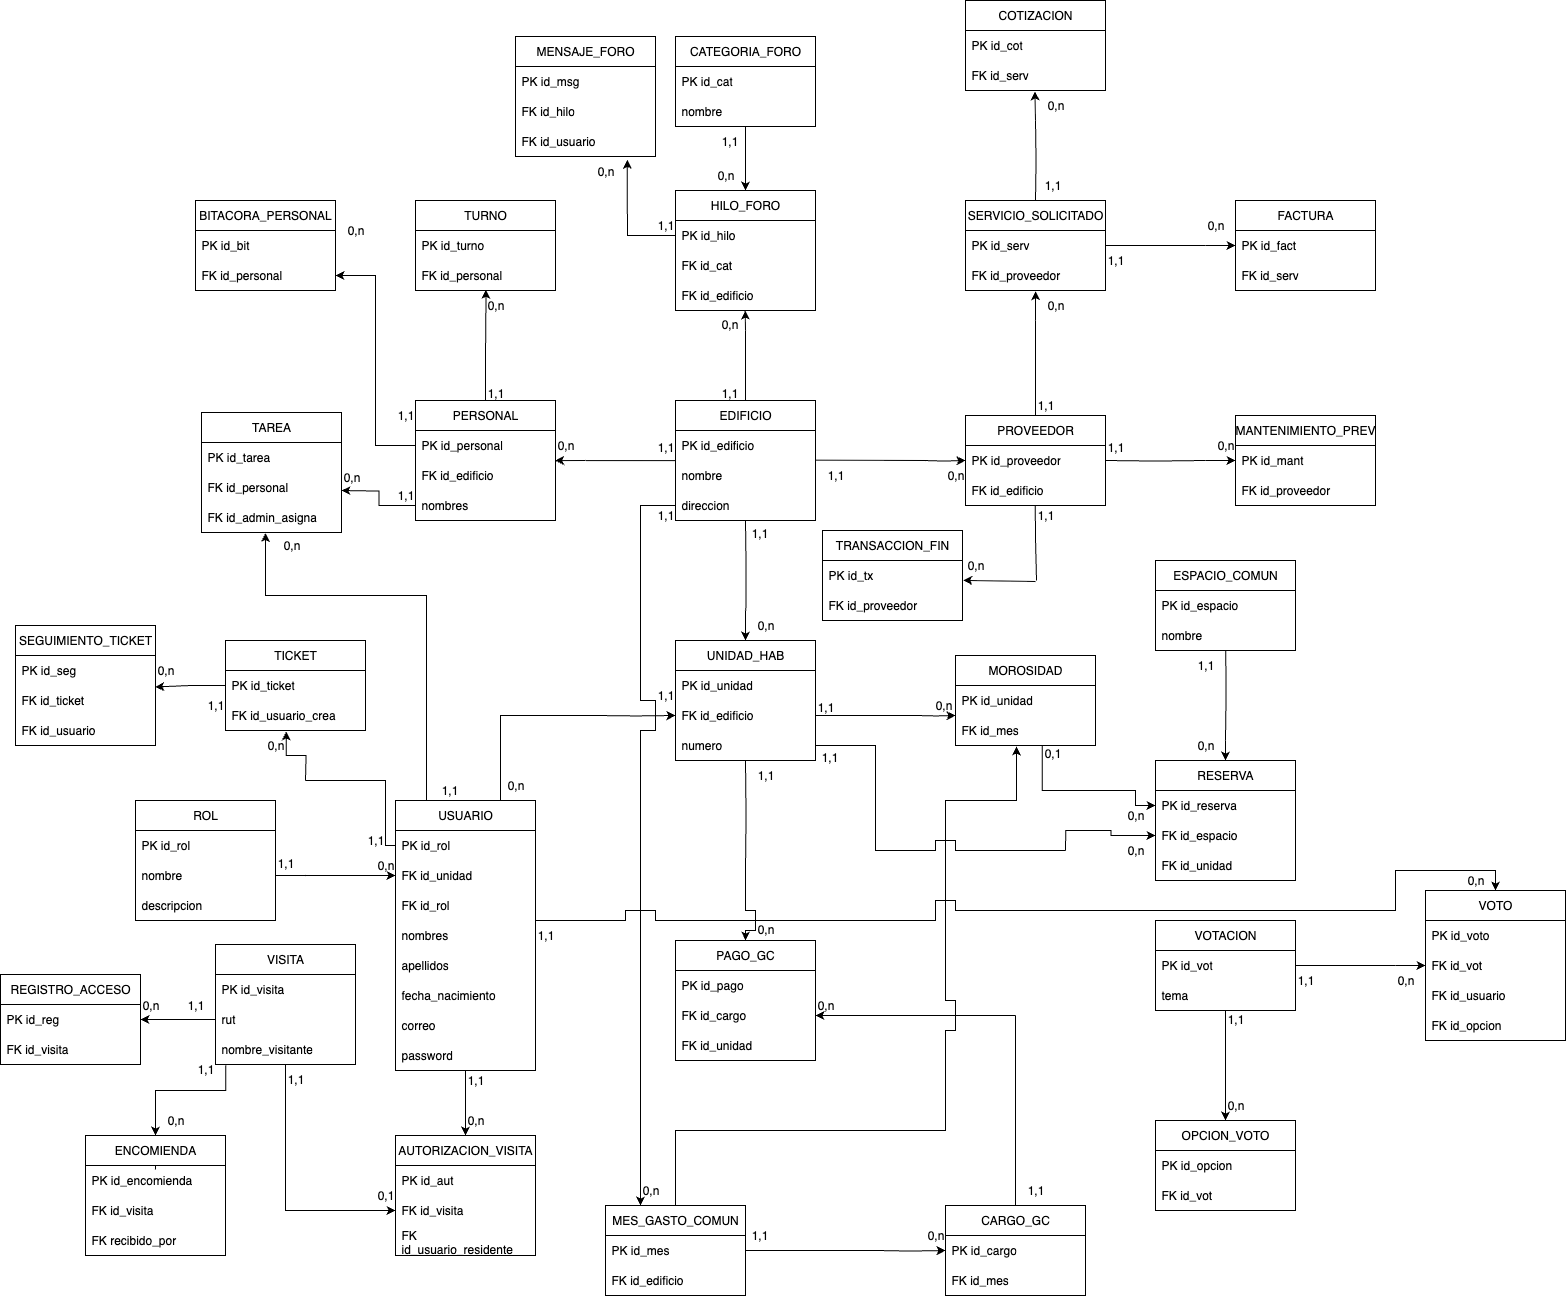
\includegraphics[width=\textwidth]{MER.png}
  \caption{Modelo Entidad-Relación del Sistema DOMU}
  \label{fig:mer}
\end{figure}

\clearpage

\cleardoublepage
\subsection{Modelo Relacional}

A continuación, se modelaron los datos siguiendo el patrón relacional, detallando las tablas, columnas, claves primarias y foráneas que se implementarán en MySQL.

\begin{figure}[H]
  \centering
  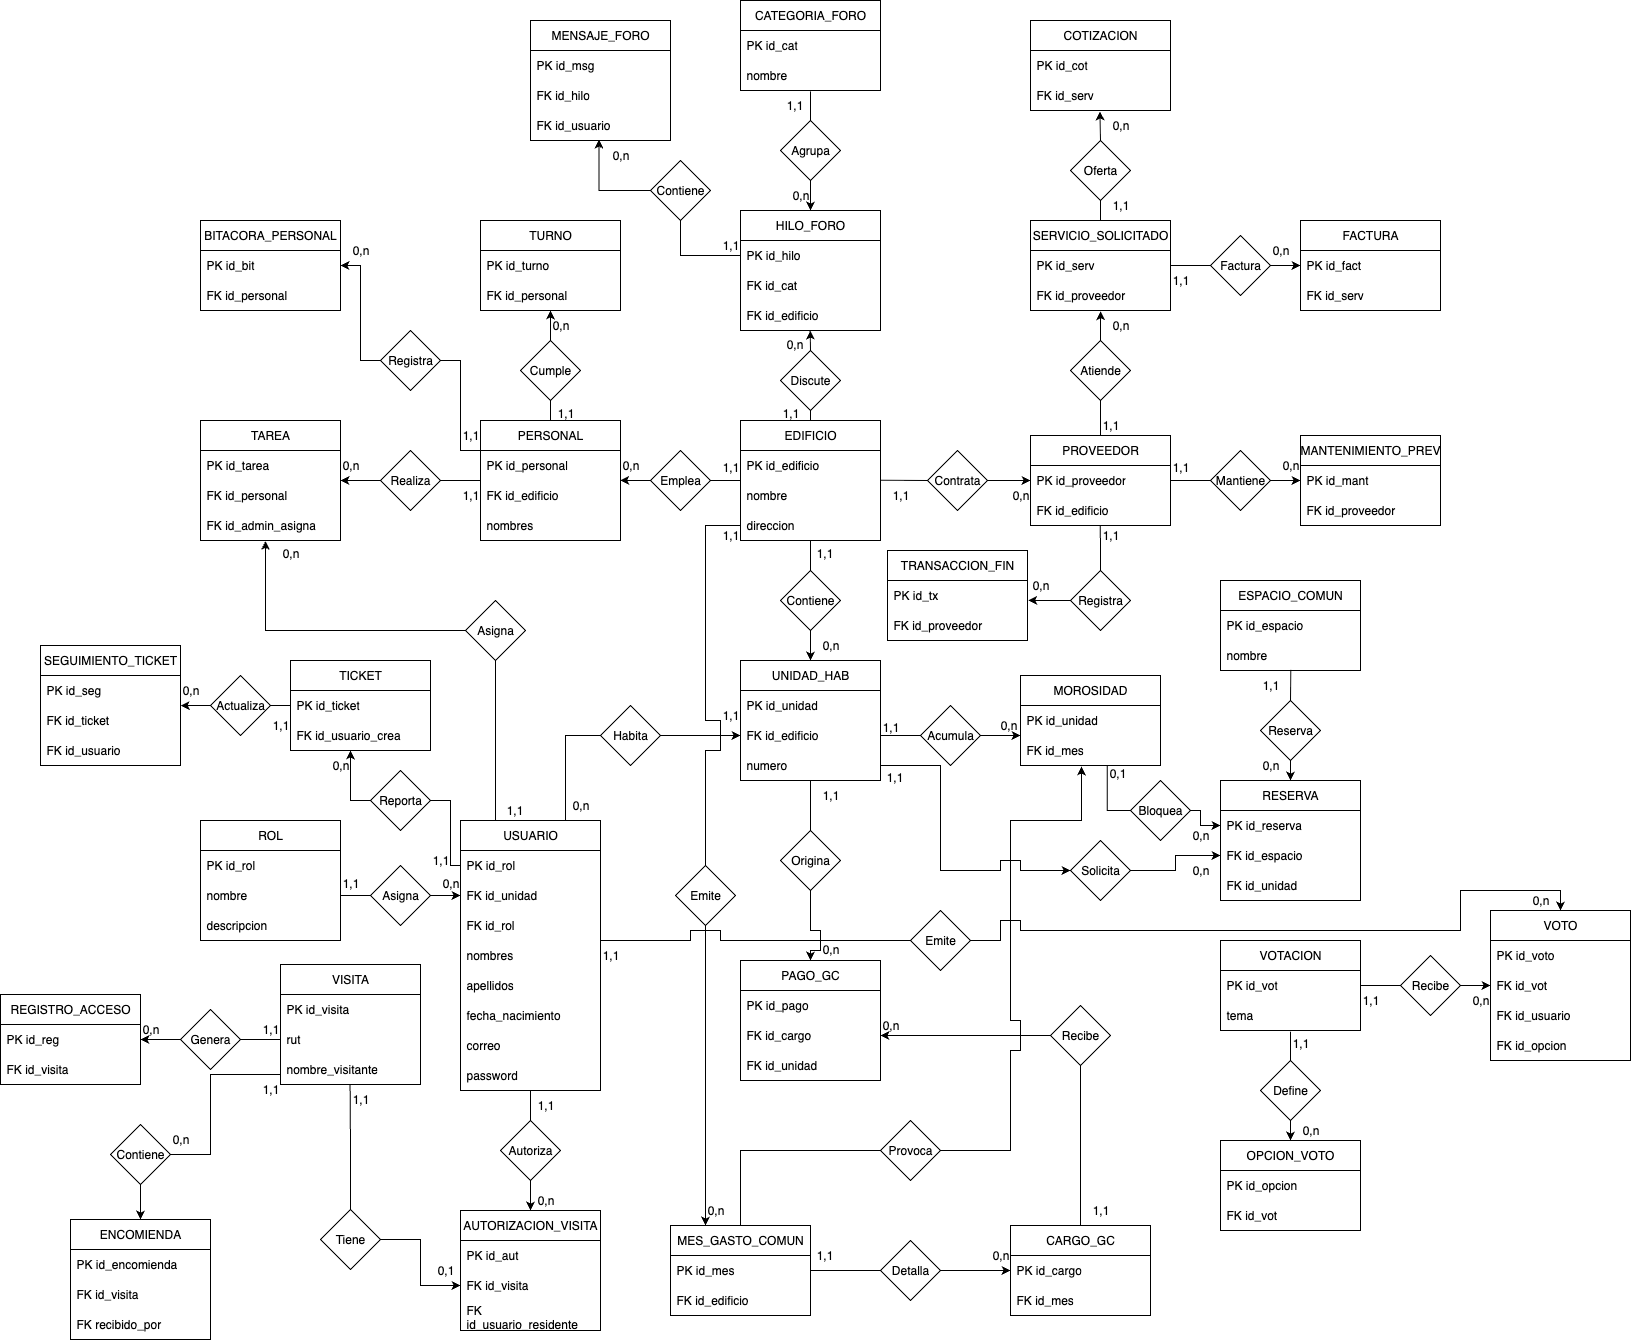
\includegraphics[width=\textwidth]{ModeloRelacional.png}
  \caption{Diagrama del Modelo Relacional del Sistema DOMU}
  \label{fig:relacional}
\end{figure}

\clearpage

\section{Diseño de interfaz y navegación}
En esta sección se dará énfasis al desarrollo de los \textit{mockups} que contempla nuestra aplicación \textbf{DOMU}, donde se detalla la guía de estilo a seguir, en conjunto con el logotipo que tendrá la \textit{app}. También se definirán las guías de colores a utilizar, las cuales serán las encargadas de representar nuestra identidad visual a través de las interfaces gráficas de la aplicación.

\subsection{Guías de estilos}

La guía de estilo marcará las pautas a seguir para el diseño de la web. Por tanto, servirá de consulta para visualizar los objetivos de la aplicación en cuanto a su estilo. El principal objetivo es dotar al estilo de la aplicación de la máxima sencillez posible, a fin de que al usuario le resulte intuitivo el uso de la aplicación. A continuación se señalarán aspectos relativos al estilo como son el logotipo, los colores principales y secundarios, la tipografía y la composición de las interfaces.

\subsection{Logotipo}
\label{subsec:logotipo}

El logotipo de \textbf{DOMU} es el principal símbolo gráfico que representa la plataforma. Podrá presentarse como \textbf{imagotipo} e \textbf{isotipo}; por defecto se utiliza exclusivamente el imagotipo a color, que combina el ícono con el nombre de la plataforma.

El ícono está basado en una letra “D” tridimensional, diseñada con geometría simple; el contorno evoca el entorno habitacional y comunitario en el que se desarrolla la aplicación.

El texto que acompaña al ícono utiliza una tipografía de estilo moderno y geométrico que refuerza la estética tecnológica de la marca.

\begin{figure}[H]
  \centering
  
\includegraphics[scale=0.5]{LogotipoDOMU.png}
  \caption{Logotipo de Domu}
  \label{fig:logo}
\end{figure}

\subsection{Guía de colores}
Los colores corporativos de la aplicación componen una gama cromática cálida, orientada a transmitir cercanía, energía y modernidad.

En conjunto, esta paleta de colores, que se muestra en la figura a continuación, busca lograr una experiencia visual agradable y llamativa para los usuarios de la plataforma.

\begin{figure}[H]
  \centering
  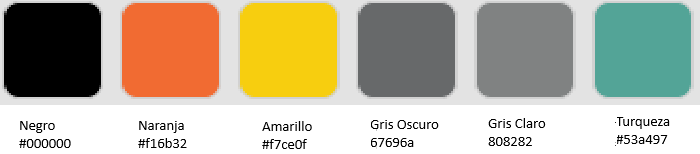
\includegraphics[scale=0.5]{PaletaDeColores.png}
  \caption{Paleta de Colores DOMU}
  \label{fig:paleta}
\end{figure}

\subsection{Tipografía}
La tipografía utilizada es un tipo de letra sencilla y universal que facilite la legibilidad. Se ha optado por emplear una fuente gratuita de Google Fonts, como es Roboto Mono. En las figuras \ref{fig:tipografia1} y \ref{fig:tipografia2} se incluye una representación de dicha fuente con los caracteres más comunes.

\begin{figure}[H]
  \centering
  
\includegraphics[scale=0.5]{EjemploTipografiaRoboto1.png}
  \caption{Texto de Ejemplo 1 Tipografía Roboto Mono}
  \label{fig:tipografia1}
\end{figure}

\begin{figure}[H]
  \centering
  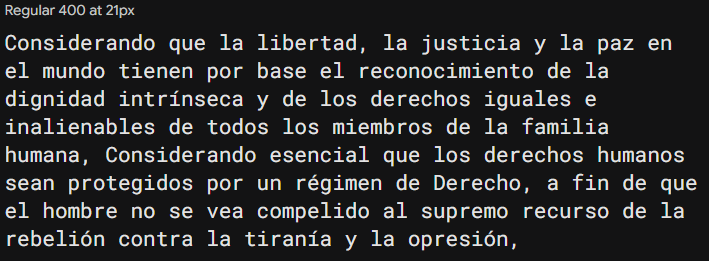
\includegraphics[scale=0.5]{EjemploTipografiaRoboto2.png}
  \caption{Texto de Ejemplo 2 Tipografía Roboto Mono}
  \label{fig:tipografia2}
\end{figure}

\subsection{Composición de Interfaces}
\label{subsec:composicion-interfaces}

La composición de las interfaces expuesta a continuación corresponde a la versión adaptada para móvil que será la versión implementada en primer lugar. La adaptación para pantallas de mayor tamaño se realizará en un futuro.

% --- ÍTEM A: Inicio de Sesión ---
\begin{itemize}
    \item[\textbf{A.}] \textbf{Inicio de Sesión (Login)}: Interfaz de autenticación para todos los usuarios.
\end{itemize}
\begin{figure}[H]
    \centering
    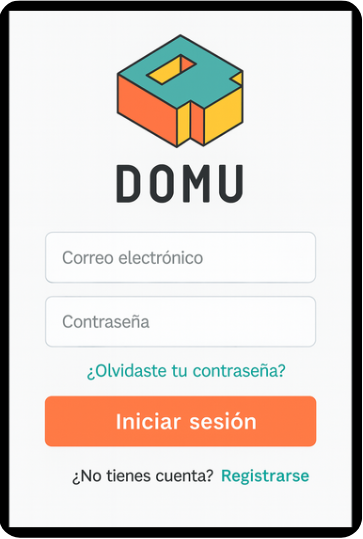
\includegraphics[scale=0.5]{InterfazInicioSesion.png}
    \caption{A. Mockup de la interfaz de Inicio de Sesión.}
    \label{fig:mockup-login}
\end{figure}
\clearpage


% --- ÍTEM B: Vista Conserje (Registro QR) ---
\begin{itemize}
    \item[\textbf{B.}] \textbf{Vista Conserje}: Interfaz operativa clave para el registro de visitas mediante escaneo QR.
\end{itemize}
\begin{figure}[H]
    \centering
    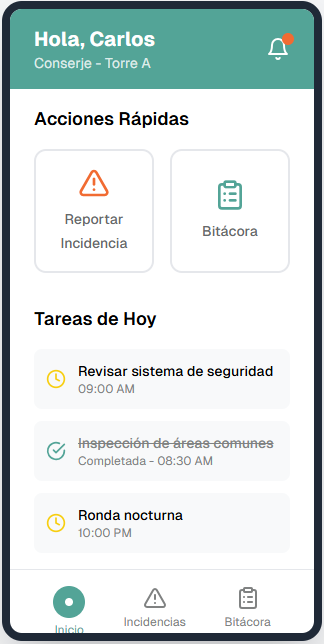
\includegraphics[scale=0.5]{InterfazConserje.png}
    \caption{B. Mockup de la interfaz de la Vista Conserje.}
    \label{fig:mockup-conserje}
\end{figure}
\clearpage


% --- ÍTEM C: Vista Administración ---
\begin{itemize}
    \item[\textbf{C.}] \textbf{Vista Administración}: Paneles de control para la gestión general de la comunidad.
\end{itemize}
\begin{figure}[H]
    \centering
    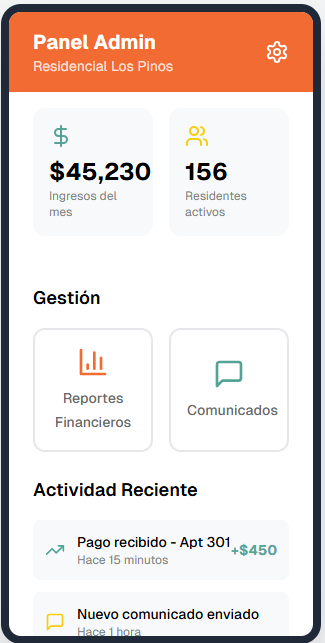
\includegraphics[scale=0.5]{InterfazAdministracion.png}
    \caption{C. Mockup de la interfaz de la Vista Administración.}
    \label{fig:mockup-administracion}
\end{figure}
\clearpage

% --- ÍTEM D: Vista Comité ---
\begin{itemize}
    \item[\textbf{D.}] \textbf{Vista Comité}: Interfaz con acceso a información crítica, documentos y procesos de votación destinados a los miembros del comité de administración.
\end{itemize}
\begin{figure}[H]
    \centering
    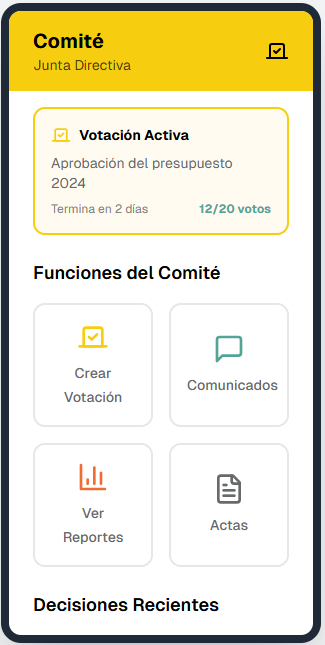
\includegraphics[scale=0.5]{InterfazComite.png}
    \caption{D. Mockup de la interfaz de la Vista Comité.}
    \label{fig:mockup-comite}
\end{figure}
\clearpage


% --- ÍTEM E: Vista Residente (Aplicación Móvil) ---
\begin{itemize}
    \item[\textbf{E.}] \textbf{Vista Residente}: Interfaz de la aplicación móvil, centralizando funcionalidades como recepción de notificaciones, reserva de espacios y pago de gastos comunes.
\end{itemize}
\begin{figure}[H]
    \centering
    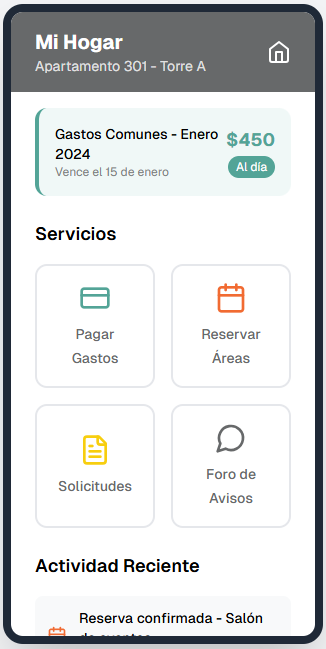
\includegraphics[scale=0.5]{InterfazResidente.png}
    \caption{E. Mockup de la interfaz de la Vista Residente (Aplicación Móvil).}
    \label{fig:mockup-residente}
\end{figure}
\clearpage


% --- ÍTEM F: Vista Reporte de Incidencias ---
\begin{itemize}
    \item[\textbf{F.}] \textbf{Vista Reporte de Incidencias}: Interfaz para la gestión y el seguimiento de reclamos, sugerencias o fallas operacionales (\textit{tickets}).
\end{itemize}
\begin{figure}[H]
    \centering
    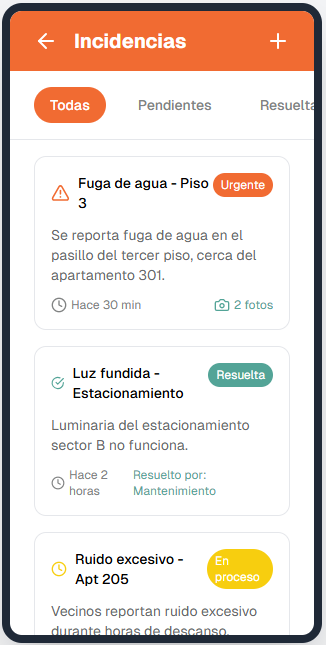
\includegraphics[scale=0.5]{InterfazReporteDeIncidencias.png}
    \caption{F. Mockup de la interfaz de Reporte de Incidencias.}
    \label{fig:mockup-incidencias}
\end{figure}
\clearpage


% --- ÍTEM G: Vista Reporte Financiero ---
\begin{itemize}
    \item[\textbf{G.}] \textbf{Vista Reporte Financiero}: Paneles analíticos que presentan a la administración las métricas clave de gastos comunes, egresos y estado de morosidad.
\end{itemize}
\begin{figure}[H]
    \centering
    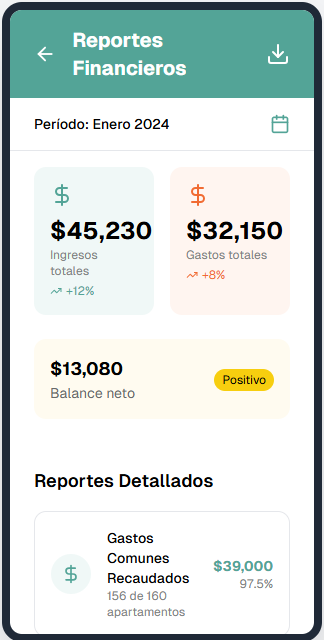
\includegraphics[scale=0.5]{InterfazReportesFinancieros.png}
    \caption{G. Mockup de la interfaz de Reporte Financiero.}
    \label{fig:mockup-financiero}
\end{figure}
\clearpage


% --- ÍTEM H: Vista Pago de Gastos Comunes ---
\begin{itemize}
    \item[\textbf{H.}] \textbf{Vista Pago de Gastos Comunes}: Flujo transaccional que guía al residente a través del proceso de pago en línea de su cuenta mensual.
\end{itemize}
\begin{figure}[H]
    \centering
    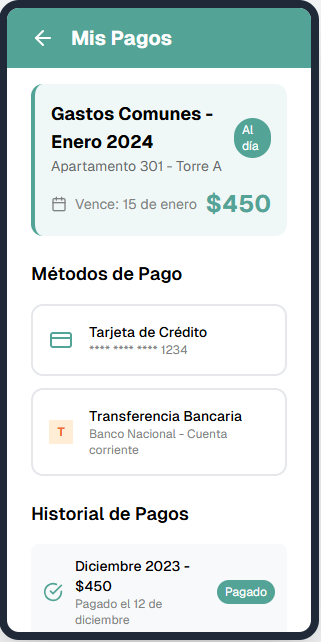
\includegraphics[scale=0.5]{InterfazPagoGGCC.png}
    \caption{H. Mockup de la interfaz de Pago de Gastos Comunes.}
    \label{fig:mockup-pago-gc}
\end{figure}
\clearpage

% --- ÍTEM I: Vista Reserva de Áreas Comunes ---
\begin{itemize}
    \item[\textbf{I.}] \textbf{Vista Reserva de Áreas Comunes}: Calendario y gestión de reservas por parte del residente.
\end{itemize}
\begin{figure}[H]
    \centering
    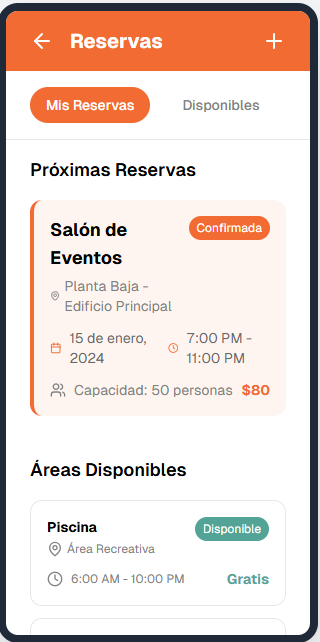
\includegraphics[scale=0.5]{InterfazReservaAreasComunes.png}
    \caption{I. Mockup de la interfaz de Reserva de Áreas Comunes.}
    \label{fig:mockup-reservas}
\end{figure}
\clearpage

\subsection{Vistas del Sistema por Rol}
\label{subsec:vistas-por-rol}

El frontend de DOMU está compuesto por \textbf{54~vistas} organizadas según el rol del usuario. A continuación se presentan las vistas agrupadas por categoría de acceso, indicando los casos de uso (CU) que cada vista materializa.

% --- Vistas Públicas ---
\begin{longtable}{|p{0.28\textwidth}|p{0.42\textwidth}|p{0.22\textwidth}|}
\caption{Vistas públicas (sin autenticación)}\label{tab:vistas-publicas}\\
\hline
\textbf{Vista} & \textbf{Descripción} & \textbf{CUs relacionados} \\
\hline
\endfirsthead
\hline \textbf{Vista} & \textbf{Descripción} & \textbf{CUs relacionados} \\ \hline
\endhead
\hline \endfoot

Home (Landing) & Página de presentación de la plataforma DOMU. & --- \\
\hline
Login & Formulario de inicio de sesión con JWT. & --- \\
\hline
Register & Registro de nuevo usuario con confirmación por correo. & --- \\
\hline
ForgotPassword & Solicitud de recuperación de contraseña. & --- \\
\hline
ConfirmEmail & Confirmación de correo electrónico vía token. & --- \\
\hline
About & Información sobre el proyecto y el equipo. & --- \\
\hline
RegisterByInvite & Registro mediante código de invitación de administrador. & CU\_24 \\

\end{longtable}

% --- Vistas Administrador ---
\begin{longtable}{|p{0.28\textwidth}|p{0.42\textwidth}|p{0.22\textwidth}|}
\caption{Vistas del Administrador}\label{tab:vistas-admin}\\
\hline
\textbf{Vista} & \textbf{Descripción} & \textbf{CUs relacionados} \\
\hline
\endfirsthead
\hline \textbf{Vista} & \textbf{Descripción} & \textbf{CUs relacionados} \\ \hline
\endhead
\hline \endfoot

AdminDashboard & Panel principal con resumen de actividad comunitaria. & CU\_09 \\
\hline
AdminCreateUser & Creación e invitación de usuarios a la comunidad. & CU\_14, CU\_24 \\
\hline
AdminIncidentsBoard & Tablero Kanban de incidentes con estados de avance. & CU\_17 \\
\hline
AdminIncidentStats & Estadísticas y métricas de incidentes reportados. & CU\_09 \\
\hline
AdminResidents & Listado y gestión de residentes por unidad. & CU\_14 \\
\hline
AdminHousingUnits & Gestión de unidades habitacionales y coeficientes. & CU\_24 \\
\hline
AdminAmenities & Configuración de áreas comunes, aforo y horarios. & CU\_05 \\
\hline
AdminCommonExpenses & Gestión de períodos, cargos y pagos de gastos comunes. & CU\_04, CU\_09 \\
\hline
AdminParcels & Gestión y seguimiento de encomiendas. & CU\_02 \\
\hline
AdminTasks & Creación y asignación de tareas al personal. & CU\_07 \\
\hline
AdminStaff & Gestión de personal operativo de la comunidad. & CU\_07 \\
\hline
AdminProviders & CRUD de proveedores vinculados a la comunidad. & CU\_19, CU\_25 \\
\hline
AdminServiceOrders & Gestión de órdenes de servicio y cotizaciones. & CU\_26 \\

\end{longtable}

% --- Vistas Conserje ---
\begin{longtable}{|p{0.28\textwidth}|p{0.42\textwidth}|p{0.22\textwidth}|}
\caption{Vistas del Conserje}\label{tab:vistas-conserje}\\
\hline
\textbf{Vista} & \textbf{Descripción} & \textbf{CUs relacionados} \\
\hline
\endfirsthead
\hline \textbf{Vista} & \textbf{Descripción} & \textbf{CUs relacionados} \\ \hline
\endhead
\hline \endfoot

VisitRegistrationPanel & Registro de visitas con escaneo QR y check-in/out. & CU\_01, CU\_15 \\
\hline
ConciergeVisitLog & Bitácora de visitas registradas. & CU\_01, CU\_03 \\
\hline
ConciergeParcels & Registro y gestión de encomiendas recibidas. & CU\_02 \\

\end{longtable}

% --- Vistas Residente ---
\begin{longtable}{|p{0.28\textwidth}|p{0.42\textwidth}|p{0.22\textwidth}|}
\caption{Vistas del Residente}\label{tab:vistas-residente}\\
\hline
\textbf{Vista} & \textbf{Descripción} & \textbf{CUs relacionados} \\
\hline
\endfirsthead
\hline \textbf{Vista} & \textbf{Descripción} & \textbf{CUs relacionados} \\ \hline
\endhead
\hline \endfoot

ResidentProfile & Perfil personal con edición de datos y avatar. & --- \\
\hline
ResidentVisits & Pre-autorización de visitas con generación de QR. & CU\_15 \\
\hline
ResidentIncidents & Reporte y seguimiento de reclamos e incidencias. & CU\_17 \\
\hline
ResidentAmenities & Consulta de disponibilidad y reserva de áreas comunes. & CU\_05 \\
\hline
ResidentCartola & Estado de cuenta del residente (gastos comunes). & CU\_04 \\
\hline
ResidentChargesDetail & Detalle de cargos por período. & CU\_04 \\
\hline
ResidentPaymentFlow & Flujo de pago de gastos comunes. & CU\_04 \\
\hline
ResidentParcels & Visualización de encomiendas pendientes y retiradas. & CU\_02 \\
\hline
ResidentPublications & Foro comunitario con categorías e hilos. & CU\_16 \\
\hline
ResidentLibrary & Biblioteca de documentos comunitarios. & CU\_22 \\
\hline
ResidentMarketplace & Marketplace de artículos entre vecinos. & CU\_21 \\
\hline
ResidentMarketplaceCreate & Publicación de nuevo artículo en marketplace. & CU\_21 \\
\hline
ChatHub & Hub de conversaciones en tiempo real (WebSocket). & CU\_20 \\
\hline
ChatRoom & Sala de chat individual con historial. & CU\_20 \\
\hline
ResidentVotaciones & Listado de votaciones activas y cerradas. & CU\_10 \\
\hline
ResidentVoteDetail & Detalle de votación con opciones y resultados. & CU\_10 \\
\hline
ResidentTasks & Visualización de tareas asignadas (rol Personal). & CU\_13 \\
\hline
ResidentContacts & Gestión de contactos frecuentes para visitas. & CU\_01 \\

\end{longtable}

% --- Vistas Proveedor ---
\begin{longtable}{|p{0.28\textwidth}|p{0.42\textwidth}|p{0.22\textwidth}|}
\caption{Vistas del Proveedor}\label{tab:vistas-proveedor}\\
\hline
\textbf{Vista} & \textbf{Descripción} & \textbf{CUs relacionados} \\
\hline
\endfirsthead
\hline \textbf{Vista} & \textbf{Descripción} & \textbf{CUs relacionados} \\ \hline
\endhead
\hline \endfoot

ProviderPortal & Portal principal del proveedor con órdenes asignadas. & CU\_27 \\
\hline
ProviderServiceOrders & Detalle de órdenes con flujo de aceptación y cotizaciones. & CU\_27 \\

\end{longtable}

% --- Vistas Especiales ---
\begin{longtable}{|p{0.28\textwidth}|p{0.42\textwidth}|p{0.22\textwidth}|}
\caption{Vistas especiales y transversales}\label{tab:vistas-especiales}\\
\hline
\textbf{Vista} & \textbf{Descripción} & \textbf{CUs relacionados} \\
\hline
\endfirsthead
\hline \textbf{Vista} & \textbf{Descripción} & \textbf{CUs relacionados} \\ \hline
\endhead
\hline \endfoot

NotificationCenter & Centro de notificaciones con lectura y preferencias. & CU\_23 \\
\hline
CommunitySelector & Selector de comunidad activa (multi-comunidad). & CU\_24 \\
\hline
UserTypeSelector & Selección de tipo de usuario en registro de proveedores. & CU\_25 \\
\hline
NotFound (404) & Página de error para rutas inexistentes. & --- \\

\end{longtable}

% === PLACEHOLDER: Reemplazar con imagen generada ===
% PROMPT para generador de imágenes (Gemini/GPT/DALL-E):
%
% "Genera un MAPA DE NAVEGACIÓN (sitemap) para una aplicación web llamada DOMU.
%
% NOTACIÓN:
% - VISTAS/PANTALLAS: rectángulos pequeños con bordes redondeados, nombre de la vista dentro.
% - ROLES: 5 franjas horizontales (swimlanes) separadas por líneas, cada una con el nombre del rol a la izquierda.
% - CONEXIONES: líneas finas conectando vistas relacionadas (ej: Cartola → ChargesDetail → PaymentFlow).
% - VISTA COMPARTIDA: el rectángulo 'NotificationCenter' cruza todas las franjas con borde punteado.
%
% FRANJAS (de arriba a abajo):
% 1. 'Público' (fondo gris claro, 7 cajas): Home, Login, Register, ForgotPassword, ConfirmEmail, About, RegisterByInvite
% 2. 'Administrador' (fondo naranja pálido, 13 cajas): Dashboard, CreateUser, IncidentsBoard, IncidentStats,
%    Residents, HousingUnits, Amenities, CommonExpenses, Parcels, Tasks, Staff, Providers, ServiceOrders
% 3. 'Conserje' (fondo verde pálido, 3 cajas): VisitRegistration, VisitLog, Parcels
% 4. 'Residente' (fondo azul pálido, 18 cajas): Profile, Visits, Incidents, Amenities, Cartola,
%    ChargesDetail, PaymentFlow, Parcels, Publications, Library, Marketplace, MarketplaceCreate,
%    ChatHub, ChatRoom, Votaciones, VoteDetail, Tasks, Contacts
% 5. 'Proveedor' (fondo morado pálido, 2 cajas): ProviderPortal, ProviderServiceOrders
%
% Las cajas dentro de cada franja se organizan en filas. Conectar con flechas finas:
% Login → (cualquier dashboard según rol). Cartola → ChargesDetail → PaymentFlow.
% ChatHub → ChatRoom. Marketplace → MarketplaceCreate. Votaciones → VoteDetail.
%
% ESTILO: Fondo blanco general, franjas con colores pastel muy suaves. Bordes de cajas en gris oscuro.
% Sin sombras ni gradientes. Tipografía sans-serif pequeña. Profesional para tesis universitaria.
% Etiquetas en español. Formato: PNG 300dpi orientación horizontal (landscape)."
\begin{figure}[H]
  \centering
  \fbox{\parbox{0.85\textwidth}{\centering\vspace{3cm}
  \textit{[Insertar diagrama: Mapa de navegación del sistema por rol --- 54 vistas organizadas por actor]}
  \vspace{3cm}}}
  \caption{Mapa de navegación del sistema DOMU segmentado por rol de usuario.}
  \label{fig:mapa-navegacion-roles}
\end{figure}

\clearpage

\section{Diseño de arquitectura}
La solución adopta un patrón de arquitectura \textbf{Cliente-Servidor} con una API RESTful como medio principal de comunicación, complementada por canales WebSocket para eventos en tiempo real. Esta separación permite que el \textit{frontend} y el \textit{backend} evolucionen, se desarrollen y se desplieguen de manera independiente, favoreciendo la mantenibilidad y la escalabilidad horizontal.

La filosofía de diseño del \textit{backend} se fundamenta en tres principios: (i)~\textbf{separación de responsabilidades} mediante una arquitectura estricta de tres capas (\textit{Controller}~$\rightarrow$~\textit{Service}~$\rightarrow$~\textit{Repository}); (ii)~\textbf{inversión de dependencias} a través del contenedor de inyección Google~Guice, que desacopla la construcción de objetos de su uso; y (iii)~\textbf{aislamiento por comunidad} (\textit{multi-tenancy} lógico) mediante el \textit{header} HTTP \texttt{X-Building-Id}, que permite que una misma instancia del servidor atienda múltiples comunidades de forma segura.

La Tabla~\ref{tab:arquitectura-componentes} detalla los componentes principales y la tecnología que los sustenta.

\begin{longtable}{|p{0.28\textwidth}|p{0.64\textwidth}|}
\caption{Componentes arquitectónicos del sistema DOMU}\label{tab:arquitectura-componentes}\\
\hline
\textbf{Componente} & \textbf{Tecnología y Responsabilidad} \\
\hline
\endfirsthead
\hline
\textbf{Componente} & \textbf{Tecnología y Responsabilidad} \\
\hline
\endhead
\hline
\endfoot

Backend (Servidor) &
Java~21 (LTS) sobre JVM. Framework Javalin~6.7 para \textit{endpoints} HTTP y WebSocket. Arquitectura interna \textit{Controller-Service-Repository} con inyección de dependencias vía Google~Guice~7.0. \\
\hline

Frontend (Cliente) &
SPA desarrollada con React~19.1 y React~Router~7.9. Empaquetado con Vite~7.1, que optimiza tiempos de carga mediante \textit{code splitting} y carga perezosa (\textit{lazy loading}). \\
\hline

Base de Datos &
MySQL~8 gestionada con HikariCP~5.1 como \textit{pool} de conexiones. Esquema versionado mediante Flyway~10.15 (35~migraciones). \\
\hline

Autenticación &
Tokens JWT (java-jwt~4.4) con firma HMAC. Contraseñas almacenadas con \textit{hash} BCrypt. Middleware \texttt{AuthenticationHandler} valida cada petición protegida. \\
\hline

WebSocket &
Dos canales persistentes: \texttt{/ws/chat} (mensajería entre usuarios) y \texttt{/ws/notifications} (alertas en tiempo real). Autenticación por token en la conexión inicial. \\
\hline

Almacenamiento en la nube &
\texttt{BoxStorageService} como capa de abstracción sobre Box~API (SDK~5.2). Servicios especializados delegan la subida de avatares, evidencias y documentos. \\
\hline

Generación de documentos &
OpenPDF~1.3.39 para la generación de boletas de gasto común, comprobantes de pago y estados de cuenta en formato PDF. \\
\hline

Correo electrónico &
Jakarta~Mail~2.0.1 para notificaciones transaccionales: confirmación de registro, aprobación de comunidades e invitaciones de administrador. \\
\hline

Serialización &
Jackson~2.17 con módulo JSR-310 para el manejo nativo de \texttt{LocalDate} y \texttt{LocalDateTime}. Configurado globalmente mediante \texttt{AppConfig.CustomJsonMapper}. \\
\hline

Multi-tenancy &
\textit{Header} \texttt{X-Building-Id} enviado por el cliente en cada petición. El \textit{middleware} inyecta el identificador de comunidad, y los repositorios filtran todas las consultas por este valor. \\

\end{longtable}

Los patrones de diseño empleados incluyen: \textbf{Repository} para encapsular el acceso a datos, \textbf{DTO} (\textit{Data Transfer Object}) para la transferencia entre capas, \textbf{Middleware} para la validación transversal de autenticación y multi-tenancy, e \textbf{Inyección de Dependencias} para el desacoplamiento y la testabilidad del código.

\subsection{Configuración Inicial del Entorno}
Para garantizar la reproducibilidad del entorno de desarrollo y la correcta ejecución del sistema, se definieron configuraciones específicas tanto para el servidor como para el cliente, eliminando dependencias obsoletas (como \texttt{pom.xml} en favor de Gradle) y estandarizando las versiones de las herramientas.

\subsubsection*{Configuración del Backend}
El proyecto \texttt{domu-backend} se gestiona mediante \textbf{Gradle~8} (usando Kotlin~DSL en \texttt{build.gradle.kts}). Las versiones de todas las dependencias se centralizan en el catálogo \texttt{gradle/libs.versions.toml}, facilitando la actualización coordinada. El empaquetado final se realiza con el \textit{plugin} \textbf{Shadow~JAR}, generando un único archivo ejecutable (\textit{fat~JAR}) que incluye todas las dependencias transitivas.

La Tabla~\ref{tab:deps-backend} detalla las dependencias de producción del backend.

\begin{longtable}{|p{0.30\textwidth}|p{0.12\textwidth}|p{0.50\textwidth}|}
\caption{Dependencias de producción del backend}\label{tab:deps-backend}\\
\hline
\textbf{Librería} & \textbf{Versión} & \textbf{Propósito} \\
\hline
\endfirsthead
\hline
\textbf{Librería} & \textbf{Versión} & \textbf{Propósito} \\
\hline
\endhead
\hline
\endfoot

Javalin & 6.7.0 & Framework web ligero para HTTP y WebSocket. \\
\hline
MySQL Connector/J & 9.0.0 & Driver JDBC para MySQL~8. \\
\hline
HikariCP & 5.1.0 & Pool de conexiones JDBC de alto rendimiento. \\
\hline
Flyway Core + MySQL & 10.15.0 & Migraciones SQL versionadas al arranque. \\
\hline
Google Guice & 7.0.0 & Contenedor de inyección de dependencias. \\
\hline
java-jwt (Auth0) & 4.4.0 & Generación y validación de tokens JWT. \\
\hline
jBCrypt & 0.4 & \textit{Hashing} seguro de contraseñas. \\
\hline
Jackson JSR-310 & 2.17.2 & Serialización JSON con soporte \texttt{LocalDate}/\texttt{LocalDateTime}. \\
\hline
Box Java SDK & 5.2.0 & Almacenamiento de archivos en Box. \\
\hline
Google Cloud Storage & 2.36.1 & Almacenamiento alternativo en GCS. \\
\hline
OpenPDF & 1.3.39 & Generación de documentos PDF (boletas, estados de cuenta). \\
\hline
Jakarta Mail & 2.0.1 & Envío de correos transaccionales (SMTP). \\
\hline
Thumbnailator & 0.4.20 & Redimensionamiento de imágenes (avatares, evidencias). \\
\hline
Log4j~2 (Core + SLF4J) & 2.23.1 & Registro de eventos (\textit{logging}) estructurado. \\
\hline
SLF4J API & 2.0.13 & Fachada de \textit{logging}. \\
\hline
Javalin OpenAPI Plugin & 6.7.0 & Generación automática de especificación OpenAPI~3 desde anotaciones. \\
\hline
Javalin Swagger Plugin & 6.7.0 & Interfaz Swagger~UI integrada para exploración interactiva de la API. \\

\end{longtable}

La configuración en tiempo de ejecución se maneja a través de variables de entorno, priorizando la seguridad (no \textit{hardcodear} credenciales). Las variables críticas definidas en \texttt{AppConfig} son: \texttt{DB\_URI}, \texttt{DB\_USER}, \texttt{DB\_PASSWORD} para la conexión JDBC; \texttt{JWT\_SECRET} para la firma de tokens; \texttt{BOX\_DEVELOPER\_TOKEN} y \texttt{BOX\_ROOT\_FOLDER\_ID} para el almacenamiento; \texttt{MAIL\_HOST}, \texttt{MAIL\_USER} y \texttt{MAIL\_PASSWORD} para el correo; y \texttt{APP\_SERVER\_PORT} para el puerto de despliegue (por defecto \textbf{8080}).

\subsubsection*{Configuración del Frontend}
El proyecto \texttt{domu-frontend} utiliza \textbf{Node.js} (v18+) como entorno de ejecución y \textbf{npm} para la gestión de paquetes. La configuración base se encuentra en \texttt{vite.config.js} y \texttt{package.json}. En entorno de desarrollo, Vite configura un \textit{proxy} que redirige todas las peticiones a \texttt{/api} hacia \texttt{http://localhost:8080}, eliminando problemas de CORS sin necesidad de configuración adicional en el backend.

La Tabla~\ref{tab:deps-frontend} detalla las dependencias del frontend.

\begin{longtable}{|p{0.32\textwidth}|p{0.12\textwidth}|p{0.48\textwidth}|}
\caption{Dependencias del frontend}\label{tab:deps-frontend}\\
\hline
\textbf{Librería} & \textbf{Versión} & \textbf{Propósito} \\
\hline
\endfirsthead
\hline
\textbf{Librería} & \textbf{Versión} & \textbf{Propósito} \\
\hline
\endhead
\hline
\endfoot

\multicolumn{3}{|l|}{\textit{\textbf{Dependencias de producción}}} \\
\hline
React & 19.1.1 & Biblioteca de construcción de interfaces de usuario. \\
\hline
React DOM & 19.1.1 & Renderizado de componentes React en el DOM. \\
\hline
React Router DOM & 7.9.4 & Enrutamiento declarativo para la SPA. \\
\hline
TanStack React Query & 5.90.21 & Gestión de estado del servidor, caché y sincronización. \\
\hline
pigeon-maps & 0.21.6 & Componente de mapas interactivos (ubicación de comunidades). \\
\hline

\multicolumn{3}{|l|}{\textit{\textbf{Dependencias de desarrollo}}} \\
\hline
Vite & 7.1.7 & Empaquetador con HMR y \textit{code splitting}. \\
\hline
@vitejs/plugin-react & 5.0.4 & Integración de React con Vite (Fast Refresh). \\
\hline
vite-plugin-pwa & 1.1.0 & Soporte PWA con \textit{Service Worker} y manifiesto. \\
\hline
Sass & 1.97.3 & Preprocesador CSS con variables y \textit{mixins}. \\
\hline
ESLint & 9.36.0 & Análisis estático de código JavaScript/JSX. \\

\end{longtable}

Se utiliza un archivo \texttt{.env} (basado en \texttt{.env.example}) para definir \texttt{VITE\_API\_BASE\_URL}, permitiendo cambiar el apuntamiento de la API entre el entorno de desarrollo local (proxy) y producción sin modificar el código fuente.

\subsection{Arquitectura de Implementación Final}

Esta sección describe cómo interactúan los componentes arquitectónicos presentados anteriormente durante la ejecución real del sistema, abordando el flujo de una petición HTTP típica, los canales WebSocket, la estrategia de almacenamiento y el mecanismo de migraciones.

\subsubsection*{Flujo de una petición HTTP}

Cada solicitud del cliente recorre las siguientes etapas antes de devolver una respuesta:

\begin{enumerate}
    \item \textbf{Cliente (React)}: El componente React invoca una función del módulo de servicios API, que utiliza \texttt{fetch} con las cabeceras \texttt{Authorization: Bearer~<token>} y \texttt{X-Building-Id:~<id>}.
    \item \textbf{Proxy de desarrollo (Vite)}: En entorno local, Vite intercepta las rutas \texttt{/api/*} y las redirige a \texttt{http://localhost:8080}, eliminando restricciones de CORS.
    \item \textbf{Javalin (Router)}: El servidor recibe la petición y la enruta al \textit{handler} correspondiente según el método HTTP y la ruta registrada.
    \item \textbf{AuthenticationHandler (Middleware)}: Valida el token JWT, extrae el identificador de usuario y lo inyecta en el contexto de la petición. Las rutas públicas (login, registro, health) se excluyen de esta validación.
    \item \textbf{Controller}: Deserializa el cuerpo de la petición mediante Jackson, valida los parámetros de entrada y delega la lógica al \textit{Service} correspondiente.
    \item \textbf{Service}: Implementa la lógica de negocio, coordina múltiples repositorios cuando es necesario y aplica el filtrado por \texttt{buildingId} para garantizar el aislamiento multi-comunidad.
    \item \textbf{Repository}: Ejecuta las consultas SQL parametrizadas contra MySQL a través del \textit{pool} de conexiones HikariCP y devuelve las entidades al \textit{Service}.
    \item \textbf{Respuesta}: El \textit{Controller} serializa el resultado como JSON (con soporte JSR-310 para fechas) y lo devuelve al cliente con el código HTTP apropiado.
\end{enumerate}

\subsubsection*{Canales WebSocket}

El sistema mantiene dos canales WebSocket persistentes, ambos autenticados mediante token JWT enviado como parámetro en la URL de conexión:

\begin{itemize}
    \item \texttt{/ws/chat}: Gestionado por \texttt{ChatWebSocketHandler}. Permite el envío y recepción de mensajes en tiempo real entre usuarios de una misma comunidad. El \textit{handler} mantiene un mapa de sesiones activas por usuario para la entrega inmediata.
    \item \texttt{/ws/notifications}: Gestionado por \texttt{NotificationWebSocketHandler}. Emite alertas en tiempo real (nuevas encomiendas, incidentes asignados, pagos registrados, etc.) según las preferencias configuradas por cada usuario.
\end{itemize}

\subsubsection*{Estrategia de almacenamiento}

Los archivos binarios (avatares, evidencias fotográficas, documentos de biblioteca) se almacenan externamente a través de \texttt{BoxStorageService}, que encapsula la interacción con la API de Box. Los servicios especializados (\texttt{UserProfileService}, \texttt{ParcelService}, \texttt{LibraryService}) delegan las operaciones de carga y descarga a esta capa centralizada, manteniendo en la base de datos únicamente la referencia (\texttt{fileId}) al recurso remoto. Las imágenes se redimensionan automáticamente mediante Thumbnailator antes de su almacenamiento.

\subsubsection*{Migraciones de base de datos}

Al arranque del servidor, Flyway escanea el directorio \texttt{db/migration} y ejecuta secuencialmente las migraciones pendientes. Cada archivo sigue la convención \texttt{V\{NNN\}\_\_descripcion.sql}, donde el prefijo numérico garantiza el orden de aplicación. El historial de migraciones se registra en la tabla interna \texttt{flyway\_schema\_history}, lo que permite detectar modificaciones manuales no autorizadas y garantizar la consistencia entre entornos.

\subsubsection*{Documentación de la API (Swagger UI)}

La API REST se documenta de forma automática mediante el plugin comunitario \textbf{javalin-openapi}, que genera una especificación OpenAPI~3 a partir de anotaciones en el código fuente. La interfaz interactiva \textbf{Swagger~UI} se encuentra disponible en la ruta \texttt{/swagger}, permitiendo a los desarrolladores explorar los endpoints, probar peticiones y consultar los esquemas de entrada/salida sin herramientas externas. La especificación JSON se expone en \texttt{/openapi} para su consumo programático.

\subsubsection*{Serialización y manejo de fechas}

La serialización JSON se configura globalmente mediante \texttt{AppConfig.CustomJsonMapper}, que registra el módulo \texttt{JavaTimeModule} de Jackson y desactiva la escritura de fechas como \textit{timestamps} numéricos. Esto permite que los tipos \texttt{LocalDate} y \texttt{LocalDateTime} se representen como cadenas ISO-8601 (e.g., \texttt{"2025-03-15"}, \texttt{"2025-03-15T14:30:00"}), facilitando su procesamiento tanto en el frontend como en integraciones externas.


\chapter{Desarrollo del Trabajo}
\label{cap:desarrollo}
Este capítulo detalla el proceso de construcción del sistema \textbf{DOMU}, describiendo la estructura técnica del código fuente, la configuración del entorno, las fases de implementación ejecutadas bajo la metodología híbrida definida y los aspectos técnicos más relevantes de la solución. Se aborda la evolución del software desde su núcleo de autenticación hasta los módulos de gestión comunitaria, financiera y de comunicación en tiempo real.

\section{Estructura del Código y Arquitectura}
\label{sec:estructura_codigo}

El sistema se ha desarrollado siguiendo una arquitectura cliente-servidor desacoplada. El Backend expone una API REST con más de 120 endpoints, consumida por el Frontend construido como una \textit{Single Page Application} (SPA). Ambos repositorios se gestionan de forma independiente mediante Git, lo que permite ciclos de desarrollo, pruebas y despliegue autónomos.

\subsection{Backend (Java)}
El servidor se ha construido con \textbf{Java~21} y el framework ligero \textbf{Javalin~6}~\cite{javalin2025}, gestionado con \textbf{Gradle} (Kotlin DSL). El proyecto cuenta con aproximadamente 190~clases Java organizadas en una arquitectura por capas. La estructura principal bajo el paquete raíz \texttt{com.domu} es la siguiente:

\begin{itemize}
    \item \textbf{config/}: Configuración global del sistema. La clase \texttt{AppConfig} centraliza los parámetros del servidor, base de datos, JWT, correo electrónico y almacenamiento en Box. La clase \texttt{DependencyInjectionModule} configura el contenedor de inyección de dependencias mediante \textbf{Google Guice}, registrando como \textit{singletons} los 27~servicios, 21~repositorios, los manejadores WebSocket y el módulo de seguridad.

    \item \textbf{domain/}: Contiene 35~entidades de dominio organizadas en subpaquetes temáticos que reflejan los módulos del sistema:
    \begin{itemize}
        \item \texttt{core/}: Entidades base (\texttt{User}, \texttt{Building}, \texttt{HousingUnit}, \texttt{Role}).
        \item \texttt{access/}: Control de acceso (\texttt{Visit}, \texttt{VisitAuthorization}, \texttt{AccessLog}, \texttt{DeliveryPackage}).
        \item \texttt{finance/}: Gestión financiera (\texttt{CommonExpensePeriod}, \texttt{CommonCharge}, \texttt{CommonPayment}, \texttt{DelinquencyRecord}).
        \item \texttt{facility/}: Áreas comunes (\texttt{CommonArea}, \texttt{Reservation}).
        \item \texttt{voting/}: Votaciones (\texttt{VotingEvent}, \texttt{VotingOption}, \texttt{Vote}).
        \item \texttt{community/}: Foro (\texttt{ForumCategory}, \texttt{ForumThread}, \texttt{ForumMessage}).
        \item \texttt{staff/}: Personal (\texttt{Personnel}, \texttt{Shift}, \texttt{Task}, \texttt{PersonnelLog}).
        \item \texttt{ticket/}: Incidentes (\texttt{Ticket}, \texttt{TicketFollowUp}).
        \item \texttt{vendor/}: Proveedores (\texttt{Provider}, \texttt{ServiceRequest}, \texttt{Quote}, \texttt{Invoice}, \texttt{PreventiveMaintenance}, \texttt{FinancialTransaction}).
    \end{itemize}

    \item \textbf{dto/}: Aproximadamente 99~\textit{Data Transfer Objects} que definen los contratos de la API. Cada módulo cuenta con DTOs de solicitud (\texttt{*Request}) y respuesta (\texttt{*Response}), separando la representación HTTP de las entidades de dominio. Ejemplos representativos incluyen \texttt{LoginRequest}, \texttt{AuthResponse}, \texttt{CreateVisitRequest}, \texttt{CommonExpensePeriodDetailResponse} y \texttt{ChatMessageResponse}.

    \item \textbf{database/}: Capa de persistencia compuesta por 21~repositorios que implementan el acceso a datos mediante JDBC directo sobre MySQL, utilizando \textbf{HikariCP}~5.1 para el \textit{pool} de conexiones. Las clases principales incluyen \texttt{UserRepository}, \texttt{CommonExpenseRepository}, \texttt{VisitRepository}, \texttt{PollRepository}, \texttt{AmenityRepository}, \texttt{ChatRepository}, \texttt{ParcelRepository}, \texttt{NotificationRepository}, entre otros. La clase \texttt{DataSourceFactory} centraliza la creación del \textit{pool} de conexiones.

    \item \textbf{service/}: Capa de lógica de negocio con 27~servicios que encapsulan las reglas del sistema. Los servicios más relevantes son:
    \begin{itemize}
        \item \texttt{UserService}: Registro, autenticación, confirmación por correo y recuperación de contraseñas.
        \item \texttt{BuildingService}: Flujo de registro de comunidades con aprobación por correo e invitación al administrador.
        \item \texttt{CommonExpenseService}: Creación de períodos de gasto común, cargos por unidad y procesamiento de pagos.
        \item \texttt{CommonExpensePdfService}, \texttt{PaymentReceiptPdfService}, \texttt{ChargeReceiptPdfService}: Generación de documentos PDF con \textbf{OpenPDF}.
        \item \texttt{VisitService}: Autorización de visitas, generación de códigos QR y \textit{check-in}.
        \item \texttt{ChatService}: Gestión de salas de chat y mensajes en tiempo real.
        \item \texttt{NotificationService}: Creación y distribución de notificaciones vía WebSocket.
    \end{itemize}

    \item \textbf{security/}: Módulo de seguridad compuesto por 4~clases: \texttt{JwtProvider} (generación y validación de tokens JWT con HMAC256), \texttt{BCryptPasswordHasher} (hashing de contraseñas), \texttt{PasswordHasher} (interfaz de abstracción) y \texttt{AuthenticationHandler} (\textit{middleware} de Javalin que intercepta las rutas protegidas y valida el token en la cabecera \texttt{Authorization}).

    \item \textbf{email/}: Servicio de correo electrónico con 6~clases: la interfaz \texttt{EmailService}, su implementación SMTP (\texttt{SmtpEmailService}) y cuatro plantillas HTML para confirmación de cuenta, aprobación de comunidades, notificación de aprobación y notificación de rechazo.

    \item \textbf{web/}: Capa de presentación HTTP con 4~clases. \texttt{WebServer} es la clase principal que registra los más de 120~endpoints REST y los dos canales WebSocket (\texttt{/ws/chat} y \texttt{/ws/notifications}). \texttt{ChatWebSocketHandler} y \texttt{NotificationWebSocketHandler} gestionan la comunicación bidireccional en tiempo real. \texttt{UserMapper} convierte entidades de usuario a DTOs de respuesta.
\end{itemize}

El esquema de base de datos se versiona mediante \textbf{Flyway}, con 35~migraciones SQL que documentan la evolución del modelo de datos desde la creación del esquema de autenticación (V001) hasta las últimas actualizaciones del sistema de notificaciones y estructura de edificios (V035).

\subsection{Frontend (React)}
La interfaz de usuario se ha construido con \textbf{React~19} y el empaquetador \textbf{Vite~7}, utilizando JavaScript (JSX) y hojas de estilo SCSS. El proyecto comprende aproximadamente 92~archivos fuente con más de 20.000~líneas de código, organizados de la siguiente manera:

\begin{itemize}
    \item \textbf{pages/} (54~vistas): Componentes de nivel de ruta que conforman las pantallas de la aplicación. Están segmentadas por rol:
    \begin{itemize}
        \item \textit{Públicas} (7): \texttt{Home}, \texttt{Login}, \texttt{Register}, \texttt{ForgotPassword}, \texttt{About}, \texttt{Contact}, \texttt{UserTypeProveedores}.
        \item \textit{Administrador} (13): \texttt{Dashboard}, \texttt{AdminCreateUser}, \texttt{AdminIncidentsBoard}, \texttt{AdminIncidentStats}, \texttt{AdminResidents}, \texttt{AdminHousingUnits}, \texttt{AdminAmenities}, \texttt{AdminCommonExpenses}, \texttt{AdminParcels}, \texttt{AdminTasks}, \texttt{AdminStaff}, \texttt{AdminProviders}, \texttt{AdminServiceOrders}.
        \item \textit{Residente} (18): \texttt{ResidentProfile}, \texttt{ResidentVisits}, \texttt{ResidentIncidents}, \texttt{ResidentAmenities}, \texttt{ResidentCartola}, \texttt{ResidentChargesDetail}, \texttt{ResidentPaymentFlow}, \texttt{ResidentParcels}, \texttt{ResidentPublications}, \texttt{ResidentLibrary}, \texttt{ResidentMarketplace}, \texttt{ChatHub}, \texttt{Votaciones}, entre otras.
        \item \textit{Proveedor} (2): \texttt{ProviderPortal}, \texttt{ProviderServiceOrders}.
        \item \textit{Especiales}: Páginas de soluciones por tipo de usuario, confirmación de correo, registro de administrador por invitación y centro de notificaciones.
    \end{itemize}

    \item \textbf{components/} (18~componentes): Elementos reutilizables de la interfaz, incluyendo \texttt{Button} (con estados de carga), \texttt{FormField} (con validación), \texttt{Spinner}, \texttt{Skeleton} (\textit{skeleton loading}), \texttt{ConfirmModal}, \texttt{LocationPicker} (selector de ubicación basado en mapas mediante la librería \texttt{pigeon-maps}), \texttt{VisitRegistrationPanel}, \texttt{MarketCard}, \texttt{ProtectedRoute} y un módulo completo de pago (\texttt{PaymentMethodModal}, \texttt{CardPaymentView}, \texttt{BankTransferView}, \texttt{ChargeSelector}, \texttt{PaymentSuccess}).

    \item \textbf{layout/} (7~componentes): Estructura visual de la aplicación, compuesta por \texttt{ProtectedLayout} (envolvente para rutas autenticadas con barra lateral y cabecera), \texttt{AuthLayout} (envolvente para páginas públicas), \texttt{Header}, \texttt{Sidebar} (navegación filtrada por rol), \texttt{Footer} y \texttt{MainContent}.

    \item \textbf{services/}: Capa de comunicación con el Backend. El archivo principal \texttt{api.js} (1.034~líneas) centraliza todas las llamadas HTTP organizadas por módulo (\texttt{auth}, \texttt{visits}, \texttt{incidents}, \texttt{finance}, \texttt{polls}, \texttt{amenities}, \texttt{chat}, \texttt{market}, \texttt{parcels}, \texttt{library}, \texttt{notifications}, entre otros). Cada petición inyecta automáticamente el token JWT en la cabecera \texttt{Authorization} y el identificador de la comunidad activa en la cabecera \texttt{X-Building-Id}.

    \item \textbf{context/}: Estado global de la aplicación mediante \textbf{React Context API}. El \texttt{AppContext} gestiona la sesión del usuario autenticado, el edificio seleccionado (soporte multi-comunidad), el tema visual (claro/oscuro) y funciones de \textit{logout} y cambio de comunidad.

    \item \textbf{hooks/}: \textit{Custom hooks} de React. El hook \texttt{useNotifications} integra WebSocket con \textbf{TanStack React Query}~v5 para recibir notificaciones en tiempo real, con reconexión automática cada 5~segundos ante desconexiones.

    \item \textbf{constants/}: Configuración centralizada con 85~definiciones de rutas, secciones de navegación filtradas por rol y 20~tipos de notificación con iconos y colores asociados.

    \item \textbf{styles/}: Hojas de estilo globales en SCSS compiladas por Vite.
\end{itemize}

La aplicación se configura como \textit{Progressive Web App} (PWA) mediante el plugin \texttt{vite-plugin-pwa}, y utiliza TanStack React Query para la gestión de caché y revalidación de datos del servidor.


\section{Fases de Implementación (Iteraciones)}
\label{sec:fases_implementacion}

Siguiendo la metodología híbrida adoptada, el desarrollo se dividió en fases iterativas que permitieron desplegar funcionalidades incrementales. Cada fase fue validada antes de avanzar a la siguiente, asegurando la estabilidad del sistema. A continuación, se describen las seis iteraciones ejecutadas.

\subsection{Fase 1: Fundamentos y Seguridad}
El objetivo de esta primera iteración fue establecer los cimientos técnicos del sistema y asegurar el acceso controlado.
\begin{itemize}
    \item \textbf{Configuración del Entorno:} Se estableció el proyecto Backend con Gradle, configurando el servidor Javalin y la conexión a MySQL mediante HikariCP. Se implementó Flyway para el versionamiento de migraciones de base de datos, asegurando la reproducibilidad del esquema entre entornos de desarrollo y producción.
    \item \textbf{Inyección de Dependencias:} Se configuró Google Guice como contenedor de inversión de control, registrando todos los servicios y repositorios como \textit{singletons} en el módulo \texttt{DependencyInjectionModule}.
    \item \textbf{Autenticación (JWT):} Se implementó un sistema de seguridad basado en \textit{JSON Web Tokens} firmados con HMAC256. Al iniciar sesión, el usuario recibe un token con una duración configurable (por defecto 60~minutos), el cual se almacena en el \texttt{localStorage} del navegador. El \textit{middleware} \texttt{AuthenticationHandler} intercepta todas las rutas protegidas y valida la vigencia del token.
    \item \textbf{Registro con Confirmación:} Se implementó el flujo completo de registro de usuarios con confirmación por correo electrónico, incluyendo el servicio SMTP con plantillas HTML (\texttt{UserConfirmationEmailTemplate}) y la recuperación de contraseñas mediante tokens de un solo uso.
    \item \textbf{Gestión de Perfiles:} Funcionalidad para que los usuarios puedan editar su información personal, cambiar su contraseña y subir avatar de perfil, con optimización automática de imágenes mediante la librería Thumbnailator.
\end{itemize}

\subsection{Fase 2: Gestión de Comunidades y Usuarios}
Se desarrollaron las herramientas administrativas necesarias para la configuración y operación de las comunidades.
\begin{itemize}
    \item \textbf{Registro de Comunidades:} Se implementó un flujo completo de solicitud, aprobación y rechazo de comunidades. La solicitud se envía mediante un formulario y la documentación se almacena en la nube mediante \textbf{Box}. El aprobador recibe un correo electrónico con enlaces para aprobar o rechazar la solicitud, tras lo cual se genera automáticamente una invitación para que el administrador de la comunidad registre su cuenta.
    \item \textbf{Soporte Multi-Comunidad:} Se diseñó un mecanismo que permite a un usuario pertenecer a múltiples edificios. El Frontend envía la cabecera \texttt{X-Building-Id} en cada petición, y el Backend filtra los datos según la comunidad activa. El contexto global del Frontend gestiona el cambio de comunidad e invalida las cachés de React Query automáticamente.
    \item \textbf{Gestión de Unidades Habitacionales:} CRUD completo de unidades (departamentos o casas) dentro de cada edificio, con la posibilidad de vincular y desvincular residentes a cada unidad.
    \item \textbf{Creación de Usuarios por Rol:} Interfaces para que el administrador pueda crear y gestionar cuentas de Conserjes, Personal de Aseo y otros funcionarios. El sistema cuenta con 5~roles base: Administrador, Residente, Conserje, Funcionario y Proveedor.
    \item \textbf{Vistas Segmentadas por Rol:} Se implementó la segmentación de la interfaz mostrando secciones de navegación y funcionalidades específicas según el rol del usuario autenticado, tanto en el \texttt{Sidebar} como en las rutas protegidas del Frontend.
\end{itemize}

\subsection{Fase 3: Servicios al Residente y Operación}
Esta fase se centró en las funcionalidades de interacción diaria dentro de la comunidad.
\begin{itemize}
    \item \textbf{Reporte y Gestión de Incidentes:} Módulo que permite a los residentes reportar problemas (filtraciones de agua, ruidos molestos, fallas eléctricas, entre otros), generando un ticket con categoría, prioridad y descripción. La administración visualiza los incidentes en un tablero tipo Kanban (\texttt{AdminIncidentsBoard}) con estados (abierto, en progreso, resuelto) y puede asignarlos a personal específico. Se implementó también una vista de estadísticas (\texttt{AdminIncidentStats}) que presenta métricas de los incidentes.
    \item \textbf{Reservas de Áreas Comunes:} Sistema de calendario que permite al administrador crear áreas comunes (quinchos, salones, gimnasios), configurar franjas horarias (\textit{time slots}) y definir aforos máximos. Los residentes pueden consultar la disponibilidad por fecha y reservar espacios desde la interfaz. Se implementó la lógica de cancelación y la restricción de reserva por morosidad.
    \item \textbf{Sistema de Votaciones:} Módulo que permite a la administración crear eventos de votación con múltiples opciones, establecer fechas de cierre y publicar resultados. Los residentes emiten su voto de manera remota. Se implementó el cierre programado de votaciones y la exportación de resultados a CSV para respaldo y auditoría.
    \item \textbf{Control de Acceso y Visitas:} Se desarrolló el módulo de autorización de visitas, permitiendo a los residentes pre-autorizar visitantes con fecha, hora y motivo. El conserje puede realizar el \textit{check-in} mediante lectura de código QR (endpoint \texttt{POST /api/visits/qr-check}) o de forma manual. Se implementó la gestión de contactos frecuentes (\texttt{VisitContactService}), que permite a los residentes guardar datos de visitantes habituales y generar visitas rápidamente a partir de ellos.
\end{itemize}

\subsection{Fase 4: Módulo Financiero}
Esta fase abordó los módulos de mayor complejidad en la lógica de negocio.
\begin{itemize}
    \item \textbf{Períodos de Gastos Comunes:} Se implementó la lógica para que el administrador cree períodos mensuales de gasto común y agregue cargos individuales por unidad habitacional, considerando el coeficiente de prorrata de cada departamento.
    \item \textbf{Flujo de Pagos:} Desarrollo completo del flujo transaccional que guía al residente a través del proceso de pago. El Frontend presenta un selector de cargos pendientes (\texttt{ChargeSelector}), opciones de método de pago (\texttt{PaymentMethodModal}) y vistas específicas para transferencia bancaria y tarjeta. El Backend procesa el pago y actualiza el estado del cargo.
    \item \textbf{Generación de Documentos PDF:} Mediante la librería \textbf{OpenPDF}, se implementaron tres servicios de generación de documentos: estados de cuenta mensuales (\texttt{CommonExpensePdfService}), comprobantes de pago (\texttt{PaymentReceiptPdfService}) y boletas de cargo (\texttt{ChargeReceiptPdfService}). Los residentes pueden descargar estos documentos directamente desde la interfaz.
    \item \textbf{Subida de Comprobantes:} Los residentes pueden subir comprobantes de transferencia bancaria, los cuales se almacenan en \textbf{Box} y quedan vinculados al cargo correspondiente para su posterior verificación por la administración.
\end{itemize}

\subsection{Fase 5: Comunicación y Módulos Comunitarios}
Se implementaron las funcionalidades orientadas a la interacción entre residentes y la vida comunitaria.
\begin{itemize}
    \item \textbf{Chat en Tiempo Real:} Sistema de mensajería instantánea construido sobre \textbf{WebSocket} (canal \texttt{/ws/chat}). El \texttt{ChatWebSocketHandler} gestiona la conexión bidireccional autenticada mediante token JWT. Los residentes pueden iniciar conversaciones con vecinos, y el sistema incluye un flujo de solicitud de chat para respetar la privacidad. Se implementó la visualización de usuarios en línea y el ocultamiento de salas.
    \item \textbf{Foro Comunitario:} Módulo de publicaciones que permite crear hilos de discusión categorizados, editarlos y eliminarlos. Funciona como un espacio de comunicación asincrónica complementario al chat.
    \item \textbf{Marketplace Comunitario:} Tienda interna que permite a los residentes publicar artículos en venta con múltiples imágenes, descripción y precio. Las imágenes se almacenan en la nube mediante \texttt{MarketplaceStorageService}. Se integra con el chat para facilitar la comunicación entre comprador y vendedor.
    \item \textbf{Gestión de Encomiendas:} Módulo para que el conserje registre la recepción de paquetes, asignándolos a la unidad habitacional correspondiente. El residente recibe una notificación y puede consultar el estado de sus encomiendas. Se implementaron cambios de estado (recibido, notificado, entregado) y la vista administrativa (\texttt{AdminParcels}).
    \item \textbf{Biblioteca de Documentos:} Repositorio digital que permite al administrador subir documentos relevantes para la comunidad (reglamentos, actas, comunicados). Los archivos se almacenan en Box y los residentes pueden descargarlos desde la interfaz.
\end{itemize}

\subsection{Fase 6: Personal, Notificaciones y Cierre}
La última iteración completó los módulos de gestión operativa y el sistema de notificaciones.
\begin{itemize}
    \item \textbf{Gestión de Personal:} CRUD completo para el registro de funcionarios (conserjes, personal de aseo, mayordomos), incluyendo la administración de turnos y la visualización del personal activo.
    \item \textbf{Asignación de Tareas:} Módulo que permite al administrador crear tareas, asignarlas a funcionarios específicos y realizar seguimiento de su estado (pendiente, en progreso, completada). Los funcionarios pueden consultar sus tareas asignadas desde la vista \texttt{StaffTasks}.
    \item \textbf{Sistema de Notificaciones en Tiempo Real:} Se implementó un canal WebSocket dedicado (\texttt{/ws/notifications}) gestionado por \texttt{NotificationWebSocketHandler}. El Backend genera notificaciones ante eventos relevantes (nueva encomienda, pago recibido, incidente actualizado, nueva visita, entre otros). El Frontend las recibe mediante el hook \texttt{useNotifications}, que integra la conexión WebSocket con TanStack React Query para mantener el estado sincronizado. Se implementó también el centro de notificaciones (\texttt{NotificationCenter}) con funcionalidad de marcar como leído y preferencias de notificación por tipo.
    \item \textbf{Servicio de Correo Electrónico:} Se consolidó el sistema de correo con plantillas HTML para confirmación de cuenta, aprobación/rechazo de comunidades y notificación al administrador invitado, utilizando Jakarta Mail sobre SMTP.
\end{itemize}

\subsection{Fase 7: Proveedores, Órdenes de Servicio y Documentación de la API}
Esta fase incorporó el módulo de gestión de proveedores externos y la documentación interactiva de la API.
\begin{itemize}
    \item \textbf{Gestión de Proveedores:} CRUD completo para registrar empresas proveedoras de servicios vinculadas a la comunidad (electricistas, gasfíteres, empresas de aseo, entre otros). El administrador puede crear, editar y desactivar proveedores desde la vista \texttt{AdminProviders}. Cada proveedor se asocia a una categoría de servicio y opcionalmente a una cuenta de usuario con rol \textit{Proveedor}.
    \item \textbf{Órdenes de Servicio:} Flujo completo de solicitud de trabajo que permite al administrador crear órdenes, asignarlas a un proveedor y realizar seguimiento por estado (pendiente, aceptada, rechazada, en progreso, completada, cancelada). El proveedor puede aceptar o rechazar órdenes, subir cotizaciones y marcar trabajos como completados desde su portal (\texttt{ProviderPortal} y \texttt{ProviderServiceOrders}).
    \item \textbf{Cotizaciones:} Los proveedores pueden adjuntar propuestas económicas a cada orden de servicio, incluyendo monto, descripción y archivo adjunto. El administrador revisa y aprueba o rechaza las cotizaciones.
    \item \textbf{Documentación de la API (Swagger~UI):} Se integró el plugin comunitario \texttt{javalin-openapi} para generar automáticamente la especificación OpenAPI~3 del sistema. La interfaz Swagger~UI, accesible en \texttt{/swagger}, permite explorar y probar los más de 130~endpoints de la API de forma interactiva.
\end{itemize}

\subsection{Contratos de la API REST}
Los contratos detallados de los endpoints principales de la API ---incluyendo
métodos HTTP, rutas, objetos de solicitud (\textit{request}) y respuesta
(\textit{response})--- se documentan en el Anexo~\ref{anexo:endpoints}.
Dicha documentación complementa la especificación interactiva disponible
en Swagger~UI y facilita la comprensión de la integración entre el Frontend
y el Backend para cada módulo funcional del sistema.

\section{Detalles Técnicos de Implementación}

\subsection{Integración del Lector de Cédula}
Para el control de acceso en conserjería, se implementó una estrategia de integración mediante hardware tipo ``pistola escáner'' de códigos QR/Barras. Este dispositivo opera en modo de emulación de teclado (\textit{HID Mode}), lo que permite su uso directo sobre el navegador web sin necesidad de controladores especiales.

El flujo técnico implementado es el siguiente:
\begin{enumerate}
    \item El conserje accede a la vista de registro de visitas en la interfaz web (\texttt{VisitRegistrationPanel}).
    \item Al escanear el código QR de la Cédula de Identidad chilena, el dispositivo ``escribe'' automáticamente la cadena de texto contenida en el código.
    \item El Frontend procesa esta cadena, extrayendo el RUN del visitante mediante \textit{parsing} de la estructura del código.
    \item Se realiza una consulta automática al Backend (endpoint \texttt{POST /api/visits/qr-check}) que verifica si la persona tiene una autorización vigente. En caso positivo, se completa el \textit{check-in} automáticamente; en caso negativo, se presenta el formulario para registro manual.
    \item Paralelamente, el sistema de contactos frecuentes (\texttt{POST /api/visit-contacts/\{id\}/register}) permite generar visitas con un solo clic para visitantes previamente guardados.
\end{enumerate}

\subsection{Manejo de Seguridad y Sesión}
La seguridad del sistema se gestiona en múltiples capas:

\begin{itemize}
    \item \textbf{Autenticación:} La clase \texttt{JwtProvider} genera tokens JWT firmados con el algoritmo HMAC256. El token contiene el identificador del usuario, su correo electrónico y una fecha de expiración configurable. Las contraseñas se almacenan encriptadas mediante \texttt{BCrypt} con sal automática.

    \item \textbf{Middleware de Autorización:} La clase \texttt{AuthenticationHandler} actúa como un \textit{before-handler} de Javalin que intercepta las peticiones a rutas protegidas. Extrae el token de la cabecera \texttt{Authorization: Bearer <token>}, lo valida y deposita el identificador del usuario en el contexto de la petición para su uso posterior por los controladores.

    \item \textbf{Interceptor en el Frontend:} El módulo \texttt{services/api.js} inyecta automáticamente el token JWT y la cabecera \texttt{X-Building-Id} en cada petición. Si el servidor responde con un código 401 (no autorizado) debido a la expiración del token, el Frontend cierra la sesión automáticamente, limpia el \texttt{localStorage} y redirige al formulario de inicio de sesión.

    \item \textbf{Recuperación de Contraseña:} Se implementó un flujo seguro de recuperación que genera un token de un solo uso almacenado en la tabla \texttt{password\_reset\_tokens}, el cual se envía por correo electrónico al usuario y expira tras su primer uso.
\end{itemize}

\subsection{Comunicación en Tiempo Real}
El sistema implementa dos canales WebSocket nativos de Javalin para comunicación bidireccional:

\begin{itemize}
    \item \textbf{Chat (\texttt{/ws/chat}):} Gestionado por \texttt{ChatWebSocketHandler}, permite el intercambio de mensajes instantáneos entre residentes. La conexión se autentica mediante el token JWT enviado como parámetro de consulta (\texttt{?token=...}). Los mensajes se persisten en la base de datos a través de \texttt{ChatRepository} y se distribuyen en tiempo real a los participantes de la sala.

    \item \textbf{Notificaciones (\texttt{/ws/notifications}):} Gestionado por \texttt{NotificationWebSocketHandler}, distribuye notificaciones a los usuarios conectados cuando ocurren eventos relevantes en el sistema. En el Frontend, el hook \texttt{useNotifications} mantiene la conexión WebSocket y sincroniza el estado con TanStack React Query, implementando reconexión automática cada 5~segundos ante desconexiones.
\end{itemize}

\subsection{Generación de Documentos PDF}
Para la generación de documentos financieros se utiliza la librería \textbf{OpenPDF}~1.3, que permite construir documentos PDF de forma programática. Se implementaron tres servicios especializados:

\begin{itemize}
    \item \texttt{CommonExpensePdfService}: Genera el estado de cuenta mensual de gastos comunes, detallando los cargos por unidad, el monto total y el período correspondiente.
    \item \texttt{PaymentReceiptPdfService}: Genera comprobantes de pago con los datos del residente, el monto pagado, la fecha y el método de pago.
    \item \texttt{ChargeReceiptPdfService}: Genera boletas individuales por cada cargo registrado.
\end{itemize}

Los documentos se generan bajo demanda cuando el residente los solicita desde la interfaz y se entregan como descarga directa a través de la API.

\subsection{Almacenamiento en la Nube}
El almacenamiento de archivos se gestiona mediante \textbf{Box}, utilizando el SDK oficial de Java con autenticación por \textit{Developer Token}. La clase central \texttt{BoxStorageService} encapsula las operaciones de subida, descarga y organización de archivos en carpetas, manteniendo una caché interna de identificadores de carpetas (\texttt{folderIdCache}) para evitar consultas redundantes a la API de Box.

Tres servicios especializados delegan en \texttt{BoxStorageService} la gestión de cada tipo de archivo:

\begin{itemize}
    \item \texttt{CommunityRegistrationStorageService}: Documentos de registro de comunidades (formularios, actas constitutivas).
    \item \texttt{CommonExpenseReceiptStorageService}: Comprobantes de pago subidos por los residentes.
    \item \texttt{MarketplaceStorageService}: Imágenes de artículos publicados en el marketplace, optimizadas automáticamente por \texttt{ImageOptimizer} antes de la subida.
\end{itemize}

Los archivos se organizan en carpetas jerárquicas dentro de Box (por edificio, módulo y entidad), y se recuperan mediante el identificador de archivo almacenado en la base de datos. Esta arquitectura permite centralizar el almacenamiento en un solo proveedor, simplificando la gestión de permisos y el mantenimiento del sistema.

\subsection{Migraciones de Base de Datos}
El esquema de base de datos se gestiona mediante \textbf{Flyway}~\cite{flyway2025}, integrado directamente en el proceso de arranque de la aplicación a través del módulo de inyección de dependencias. Al iniciar el servidor, Flyway ejecuta automáticamente las migraciones pendientes, asegurando que el esquema esté siempre sincronizado con la versión del código.

El proyecto cuenta con 35~migraciones versionadas (V001 a V035) que documentan la evolución completa del modelo de datos: desde la creación del esquema de autenticación y roles, pasando por la incorporación de visitas, incidentes, votaciones, áreas comunes, finanzas, marketplace, chat, foro, encomiendas, tareas, personal, biblioteca, notificaciones, proveedores y órdenes de servicio, y las optimizaciones de rendimiento (índices y ajustes de esquema). El detalle completo de cada migración se presenta en el Anexo~\ref{anexo:diccionario}.

\section{Conclusión del Capítulo}
El sistema \textbf{DOMU} ha completado las siete fases de desarrollo planificadas, alcanzando un estado funcional completo con más de 130~endpoints REST, dos canales WebSocket, 35~migraciones de base de datos y una interfaz de usuario compuesta por 54~vistas. Los módulos de autenticación, gestión de comunidades, control de acceso, finanzas, incidentes, votaciones, reservas, chat, foro, marketplace, encomiendas, tareas, personal, biblioteca, notificaciones, proveedores y órdenes de servicio se encuentran operativos e integrados. Adicionalmente, la API se documenta de forma interactiva mediante Swagger~UI. El siguiente paso corresponde a las pruebas de aceptación, el despliegue en producción y la marcha blanca descritos en el capítulo siguiente.


\chapter{Implantación y Puesta en Marcha}
\label{cap:implantacion}
Este capítulo describe la estrategia técnica y operativa para el despliegue del sistema DOMU en un entorno productivo, asegurando su disponibilidad, seguridad y correcta adopción por parte de la comunidad.

\section{Arquitectura de Despliegue}

Para la puesta en marcha se ha diseñado una arquitectura basada en contenedores Docker, lo que garantiza la portabilidad del sistema y facilita el escalado horizontal. La Figura~\ref{fig:despliegue} ilustra los componentes del despliegue.

\begin{figure}[H]
\centering
\begin{tabular}{|p{0.92\linewidth}|}
\hline
\textbf{Diagrama de Despliegue --- DOMU} \\[4pt]
\texttt{[Cliente Web]} $\longrightarrow$ \texttt{CDN (Vercel/Netlify)} $\longrightarrow$ \texttt{SPA React} \\[2pt]
\texttt{[Cliente Móvil]} $\longrightarrow$ \texttt{PWA (navegador móvil, instalable en inicio)} \\[2pt]
\texttt{[Conserjería]} $\longrightarrow$ \texttt{Navegador + Pistola QR} \\[6pt]
\hfill $\downarrow$ \texttt{HTTPS / WSS} $\downarrow$ \hfill \\[4pt]
\texttt{[Servidor de Aplicaciones]} \\
\quad \texttt{Docker: eclipse-temurin:21-alpine} \\
\quad \texttt{Javalin 6 (API REST + WebSocket)} \\
\quad \texttt{Puerto 7070} \\[4pt]
\hfill $\downarrow$ \texttt{JDBC} $\downarrow$ \hfill \\[4pt]
\texttt{[Base de Datos]} \texttt{MySQL 8.0 (AWS RDS / Cloud SQL)} \\[4pt]
\texttt{[Almacenamiento]} \texttt{Box (archivos, comprobantes, imágenes)} \\
\hline
\end{tabular}
\caption{Arquitectura de despliegue del sistema DOMU.}
\label{fig:despliegue}
\end{figure}

Los componentes principales del despliegue son los siguientes:

\begin{itemize}
    \item \textbf{Servidor de Aplicaciones:} El backend Java se empaqueta en una imagen Docker basada en \texttt{eclipse-temurin:21-alpine}, optimizada para bajo consumo de recursos. Se despliega en un servicio de orquestación como AWS ECS o en un VPS con Docker Compose. La imagen expone el puerto~7070 y se configura mediante variables de entorno para los parámetros de base de datos, JWT, correo electrónico y almacenamiento.

    \item \textbf{Base de Datos:} Se utiliza una instancia gestionada de MySQL~8.0 en la nube (AWS RDS o Google Cloud SQL) para garantizar copias de seguridad automáticas, alta disponibilidad y mantenimiento delegado al servicio administrado. La conexión desde el servidor de aplicaciones se realiza mediante JDBC con HikariCP como pool de conexiones.

    \item \textbf{Frontend Web:} La aplicación React se construye como una SPA (\textit{Single Page Application}) y se distribuye a través de una red de entrega de contenido (CDN) como Vercel o Netlify. El proceso de \textit{build} genera archivos estáticos optimizados que se sirven directamente desde la CDN, reduciendo la latencia para los usuarios finales.

    \item \textbf{Aplicación Móvil (PWA):} La experiencia móvil se implementa como una \textit{Progressive Web App} (PWA). Los usuarios acceden desde el navegador de su dispositivo móvil y pueden instalar la aplicación en la pantalla de inicio para una experiencia similar a una app nativa, sin necesidad de distribución por tiendas de aplicaciones. La PWA se sirve desde la misma CDN que el frontend web, simplificando el despliegue y la actualización.

    \item \textbf{Almacenamiento de Archivos:} Los archivos estáticos (evidencias, comprobantes de pago, fotos de perfil, imágenes del marketplace) se alojan en Box, configurado con políticas de acceso privado y URLs firmadas temporalmente para la descarga segura.
\end{itemize}

\subsection{Configuración Docker}

El servidor de aplicaciones se despliega mediante un archivo \texttt{docker-compose.yml} que define los servicios, redes y volúmenes necesarios. La configuración incluye:

\begin{itemize}
    \item Servicio \texttt{domu-api}: imagen Docker del backend con variables de entorno para la configuración de base de datos, JWT, SMTP y Box.
    \item Servicio \texttt{mysql}: instancia de MySQL~8.0 con volumen persistente para los datos (utilizado en desarrollo; en producción se reemplaza por una instancia gestionada).
    \item Red interna \texttt{domu-network}: aísla la comunicación entre los servicios del sistema.
\end{itemize}

\subsection{Gestión de Migraciones}

Al iniciar el contenedor del backend, Flyway ejecuta automáticamente las migraciones de base de datos pendientes (35~migraciones versionadas, V001 a V035). Este mecanismo asegura que el esquema de la base de datos esté siempre sincronizado con la versión del código desplegado, eliminando la necesidad de scripts manuales de actualización.

\section{Plan de Capacitación}

La adopción del sistema requiere nivelar las competencias digitales de los distintos usuarios. Se diseñó un plan de capacitación diferenciado por perfil de usuario.

\subsection{Administración y Comité}
Se realiza una sesión de inducción de 2~horas enfocada en la configuración inicial del edificio: carga de la nómina de residentes, configuración de alícuotas, definición de áreas comunes, creación de períodos de gastos comunes y generación de estados de cuenta. Para el Comité, la capacitación considera explícitamente los flujos de gobernanza comunitaria implementados en la plataforma, manteniendo consistencia con los casos de uso y diseño funcional definidos en capítulos previos.
\begin{itemize}
    \item \textbf{Generación de votaciones:} creación de procesos de votación, definición de opciones, cierre y publicación de resultados desde el módulo de votaciones.
    \item \textbf{Carga de actas de asamblea:} publicación de documentos en biblioteca con la etiqueta obligatoria \texttt{actas}, siguiendo la trazabilidad documental del sistema.
    \item \textbf{Consulta de estados de cuenta:} revisión de estados de cuenta en modo fiscalización para seguimiento financiero comunitario.
\end{itemize}
Se entrega un manual de gestión en formato digital con procedimientos separados para Administración y Comité, incluyendo prácticas operativas y criterios de uso por rol.

\subsection{Personal de Conserjería}
Capacitación práctica en terreno (30~minutos) centrada exclusivamente en el uso del módulo de Control de Accesos y la operación de la pistola lectora de QR. Se prioriza la rapidez operativa para no entorpecer el flujo de ingreso de personas. La capacitación incluye:
\begin{itemize}
    \item Inicio de sesión y navegación básica.
    \item Registro de visitas mediante escaneo QR de cédula de identidad.
    \item Verificación de pre-autorizaciones de visitas.
    \item Registro manual de visitas sin cédula (visitantes extranjeros o cédulas deterioradas).
    \item Recepción y registro de encomiendas.
\end{itemize}

\subsection{Residentes}
Se distribuye un video tutorial de 3~minutos vía WhatsApp y correo electrónico, explicando cómo descargar la aplicación, registrarse, recuperar la contraseña, pre-autorizar una visita, registrar una reserva de área común y consultar el estado de gastos comunes. Adicionalmente, se habilita una sección de ayuda dentro de la aplicación con preguntas frecuentes.

\section{Estrategia de Lanzamiento}

Se recomienda una estrategia de \textbf{marcha blanca} de dos semanas, diseñada para minimizar el riesgo de la transición y permitir una adopción gradual del sistema.

\begin{enumerate}
    \item \textbf{Semana~1 (Paralelo):} El sistema DOMU funciona simultáneamente con el libro de visitas manual y los procesos vigentes. No se bloquean accesos ni se cobran multas asociadas al sistema digital. El objetivo es poblar la base de datos con residentes, unidades habitacionales y contactos frecuentes, y habituar al personal de conserjería a la operación del escáner QR.

    \item \textbf{Semana~2 (Transición):} Se elimina el registro en papel para visitas y encomiendas. Se habilita el módulo de reservas de áreas comunes. Los residentes comienzan a recibir notificaciones y a interactuar con la plataforma. En paralelo, Administración y Comité ejecutan una validación operativa guiada de los flujos de votaciones, carga de actas y consulta de estados de cuenta. Se monitorean incidencias y se resuelven en tiempo real.

    \item \textbf{Lanzamiento Oficial:} Se habilita el módulo financiero para el siguiente ciclo de facturación mensual. Se genera el primer estado de cuenta a través del sistema, se activan los flujos de pago y queda operativo el uso regular de los flujos de gobernanza por parte del Comité.
\end{enumerate}

\section{Respaldo y Recuperación}

Para garantizar la integridad de la información, se implementa la siguiente estrategia de respaldo:

\begin{itemize}
    \item \textbf{Respaldo de base de datos:} Se configuran rutinas automáticas (\textit{cron jobs}) que ejecutan un respaldo completo diario (\texttt{mysqldump}) de la base de datos MySQL. Los archivos de respaldo se comprimen y almacenan en un \textit{bucket} de almacenamiento en la nube (Google Drive o AWS~S3) con retención de 30~días.

    \item \textbf{Respaldo de archivos:} Los documentos almacenados en Box cuentan con redundancia y versionado nativo del servicio, garantizando la recuperación ante eliminaciones accidentales.

    \item \textbf{Objetivo de punto de recuperación (RPO):} 24~horas. En caso de fallo, se puede restaurar la base de datos al estado del último respaldo diario.

    \item \textbf{Objetivo de tiempo de recuperación (RTO):} 2~horas. El procedimiento de recuperación consiste en: (1)~restaurar el respaldo en una nueva instancia de MySQL, (2)~verificar la integridad de los datos, y (3)~reapuntar el servidor de aplicaciones a la nueva instancia.
\end{itemize}

\section{Monitoreo y Mantenimiento}

\begin{itemize}
    \item \textbf{Logs de aplicación:} El servidor Javalin registra todas las solicitudes HTTP y eventos del sistema en la salida estándar del contenedor Docker. Los logs se recopilan mediante el driver de logging de Docker y pueden integrarse con servicios de monitoreo como CloudWatch o Datadog.

    \item \textbf{Métricas de salud:} Se expone un endpoint \texttt{/health} que verifica la conectividad con la base de datos y el estado del servidor. Este endpoint es utilizado por el orquestador de contenedores para detectar y reiniciar instancias no saludables.

    \item \textbf{Monitoreo funcional de implantación:} Durante la marcha blanca se supervisan además los flujos críticos por perfil, incluyendo las operaciones de Administración y Comité sobre votaciones, biblioteca documental (etiqueta \texttt{actas}) y consulta de estados de cuenta.

    \item \textbf{Mantenimiento correctivo:} Las correcciones de errores (\textit{hotfixes}) se despliegan mediante la construcción de una nueva imagen Docker y la actualización del servicio en el orquestador, proceso que no requiere tiempo de inactividad gracias al despliegue \textit{rolling}.

    \item \textbf{Mantenimiento evolutivo:} Las nuevas funcionalidades se desarrollan en ramas independientes, se prueban en un entorno de staging y se despliegan en producción siguiendo el mismo proceso de actualización de imágenes Docker.
\end{itemize}

\section{Plan de Rollback}

En caso de que el despliegue presente fallos críticos que afecten la operación del sistema, se ejecuta el siguiente procedimiento de reversión:

\begin{enumerate}
    \item Revertir la imagen Docker del servidor de aplicaciones a la versión anterior mediante el tag de la imagen previamente etiquetada.
    \item Si la nueva versión incluyó migraciones de base de datos incompatibles, restaurar el respaldo diario más reciente de la base de datos.
    \item Verificar el correcto funcionamiento del sistema con la versión anterior, incluyendo validación de los flujos críticos de Administración y Comité.
    \item Comunicar a los usuarios afectados sobre la interrupción temporal del servicio.
\end{enumerate}

\section{Limitaciones del Despliegue}

Se identifican las siguientes limitaciones en la estrategia de despliegue de la versión~1.0:

\begin{itemize}
    \item \textbf{Ausencia de pipeline CI/CD:} El proceso de construcción y despliegue de imágenes Docker se realiza de forma manual. La implementación de un pipeline automatizado mediante GitHub Actions se contempla como trabajo futuro.
    \item \textbf{Limitaciones de la PWA:} Al ser una Progressive Web App, algunas funcionalidades nativas (como notificaciones push en iOS pre-16.4 y acceso a cierto hardware) no están disponibles. Sin embargo, la cobertura de navegadores modernos es suficiente para el público objetivo del sistema.
    \item \textbf{Instancia única:} En la versión~1.0, el servidor de aplicaciones opera como instancia única sin balanceo de carga. Para escenarios de alta concurrencia, se requiere configurar múltiples réplicas del servicio.
\end{itemize}


\chapter{Conclusión}
\label{cap:conclusion}
% Capítulo 9 – Conclusión

Este capítulo presenta las conclusiones del proyecto DOMU, evaluando el grado de cumplimiento de los objetivos planteados, las competencias desarrolladas, las dificultades enfrentadas y las líneas de trabajo futuro.

\section{Cumplimiento de los Objetivos}

\subsection{Evaluación de los Objetivos Específicos}

A continuación se evalúa el cumplimiento de cada uno de los seis objetivos específicos definidos en el Capítulo~1:

\begin{enumerate}
    \item \textbf{Comparar los sistemas actuales de administración de edificios, identificando sus fortalezas y limitaciones, para definir los requerimientos funcionales de la propuesta.}

    \textit{Cumplido.} Se investigaron y documentaron cuatro plataformas del mercado chileno: ComunidadFeliz, Edifito, Edipro y GastoComunChile (Capítulo~1, §1.4). Se identificaron sus fortalezas (digitalización financiera, comunicación con residentes) y sus debilidades (modularización comercial, falta de integración operativa). A partir de este análisis y de la retroalimentación recogida, se definieron 20~requerimientos funcionales (Capítulo~3, §3.4) que abordan las brechas detectadas.

    \item \textbf{Definir tecnologías y metodologías que permitan desarrollar el sistema de registro con escaneo QR, página web y backend.}

    \textit{Cumplido.} Se seleccionó un stack tecnológico compuesto por Java~21 con Javalin~6 para el backend, React con JavaScript y SCSS para el frontend web, una Progressive Web App (PWA) para la experiencia móvil y MySQL~8.0 como motor de base de datos (Capítulo~2, §2.5). Se adoptó una metodología híbrida Cascada--Iterativa (Capítulo~2, §2.2) que combinó la rigurosidad documental de la fase de análisis con la flexibilidad de ciclos cortos de construcción. Se evaluó e integró exitosamente una pistola escáner QR como periférico de captura, verificando su compatibilidad con el estándar ISO/IEC~18004 y el formato de la cédula de identidad chilena.

    \item \textbf{Diseñar la estructura de software que incorpora módulos de control de acceso, seguimiento de encomiendas, asignación de tareas al personal y comunicación con los residentes.}

    \textit{Cumplido.} Se diseñó una arquitectura cliente--servidor desacoplada con API REST (Capítulo~6, §6.4), un modelo de datos compuesto por 35~entidades organizadas en 9~dominios (Capítulo~6, §6.2), diagramas BPMN~2.0 de los procesos clave (Capítulo~1, §1.2), un modelo entidad--relación completo (Capítulo~6, §6.2.2) y 9~mockups de las interfaces principales (Capítulo~6, §6.3.5). La arquitectura integra los módulos de control de acceso, encomiendas, finanzas, incidentes, votaciones, reservas, chat, foro, marketplace, tareas, personal y proveedores en un diseño cohesivo.

    \item \textbf{Implementar un prototipo funcional que integre los módulos diseñados en una plataforma inicial.}

    \textit{Cumplido.} El sistema fue construido en siete fases de implementación progresiva (Capítulo~7, §7.2), alcanzando un estado funcional completo con más de 130~endpoints REST, 2~canales WebSocket, 35~migraciones de base de datos y 54~vistas de interfaz de usuario. Todos los módulos se encuentran operativos e integrados, y la API se documenta de forma interactiva mediante Swagger~UI.

    \item \textbf{Integrar el software de registro con el hardware de escaneo QR, verificando la correcta captura, parseo y envío de los datos de la cédula de identidad.}

    \textit{Cumplido.} Se implementó exitosamente la integración del escáner QR con el módulo de control de accesos (Capítulo~7, §7.3.1). La pistola lectora opera en modo de emulación de teclado, capturando la cadena de texto codificada en el QR de la cédula chilena. El software realiza el \textit{parsing} del contenido, extrayendo los campos relevantes (RUT, nombre, apellidos) y registrando el acceso en la base de datos en menos de cinco segundos. Se validó la precisión de la captura con múltiples cédulas de identidad.

    \item \textbf{Realizar pruebas finales, validación y ajuste del sistema DOMU.}

    \textit{Cumplido parcialmente.} Se diseñaron y ejecutaron pruebas funcionales durante cada fase de desarrollo, verificando el correcto funcionamiento de los módulos implementados. Las pruebas de aceptación de usuario se presentan en el Anexo~B. Sin embargo, las pruebas en un entorno productivo real con usuarios finales de una comunidad se encuentran pendientes para la etapa de marcha blanca (Capítulo~8, §8.3).
\end{enumerate}

\subsection{Evaluación del Objetivo General}

El objetivo general del proyecto consistía en desarrollar una plataforma web integral para la administración de comunidades residenciales que integrara y optimizara los procesos críticos: registro y verificación de visitas con pre-autorización y control de acceso, trazabilidad de encomiendas, gestión de gastos comunes, asignación y seguimiento de tareas, reporte de incidentes, reserva de áreas comunes, y comunicación interna mediante foro, chat y marketplace comunitario.

Se concluye que el objetivo general ha sido \textbf{alcanzado en su totalidad} en lo que respecta al desarrollo del software. La plataforma DOMU integra todos los módulos planificados en un entorno centralizado, con trazabilidad de la información y acceso diferenciado para administradores, conserjes y residentes. El sistema se encuentra funcional y listo para su despliegue en producción.

\section{Tiempo y Esfuerzo}

El proyecto fue planificado para un periodo de desarrollo de cuatro meses con dedicación parcial (40~horas mensuales por integrante), totalizando 320~horas--persona de desarrollo directo.

La distribución real del esfuerzo evidenció que las fases de implementación del backend y la integración de módulos demandaron más tiempo del estimado inicialmente, debido a la complejidad de la lógica financiera (cálculo de gastos comunes, generación de PDF, gestión de períodos contables) y la integración del almacenamiento con Box. En contrapartida, el desarrollo del frontend fue más ágil de lo previsto gracias a la adopción de TanStack React Query para la gestión del estado del servidor, lo que redujo significativamente el código \textit{boilerplate}.

La carta Gantt del Anexo~A refleja las desviaciones entre la planificación original (anteproyecto) y la ejecución real del proyecto, evidenciando ajustes en la priorización de módulos pero manteniendo la fecha de cierre global.

\section{Competencias Desarrolladas}

El desarrollo de este proyecto de título permitió fortalecer y aplicar competencias clave del perfil de egreso de Ingeniería Civil en Informática de la Universidad del Bío-Bío:

\begin{itemize}
    \item \textbf{Diseño y desarrollo de soluciones de software:} Se diseñó e implementó un sistema completo desde la especificación de requerimientos hasta el despliegue, aplicando patrones de arquitectura (API REST, inyección de dependencias, DTOs) y buenas prácticas de ingeniería de software.

    \item \textbf{Gestión de proyectos:} Se planificó y ejecutó el proyecto utilizando una metodología híbrida, gestionando plazos, priorizando funcionalidades y documentando el proceso conforme a estándares IEEE.

    \item \textbf{Modelado de procesos de negocio:} Se utilizó BPMN~2.0 para representar los procesos del ámbito residencial, vinculando los flujos de negocio con los requerimientos del software.

    \item \textbf{Evaluación de factibilidad:} Se realizó un análisis de factibilidad técnica, operativa y económica completo, incluyendo proyecciones financieras, cálculo de VAN y estimación de costos de desarrollo.

    \item \textbf{Integración de tecnologías:} Se logró integrar múltiples tecnologías heterogéneas (Java, React, PWA, MySQL, WebSocket, Box, OpenPDF, Flyway, escáner QR) en una solución cohesiva.

    \item \textbf{Comunicación técnica:} La elaboración del presente informe y la documentación del sistema contribuyeron a desarrollar la capacidad de comunicar decisiones técnicas de forma clara y fundamentada.
\end{itemize}

\section{Dificultades Encontradas}

Durante el desarrollo del proyecto se enfrentaron diversas dificultades que requirieron adaptación y creatividad para su resolución:

\begin{itemize}
    \item \textbf{Complejidad del módulo financiero:} La lógica de cálculo de gastos comunes, con sus múltiples tipos de cargos (fijos, proporcionales, extraordinarios), la generación de estados de cuenta en PDF y la gestión de períodos contables resultó significativamente más compleja de lo previsto. Se requirieron varias iteraciones de diseño para lograr un modelo de datos flexible y correcto.

    \item \textbf{Integración del escáner QR:} El \textit{parsing} de la cadena de texto del código QR de la cédula chilena presentó variaciones de formato entre emisiones de distintos años del Servicio de Registro Civil e Identificación, lo que obligó a implementar una lógica de extracción robusta con múltiples patrones de reconocimiento.

    \item \textbf{Comunicación en tiempo real:} La implementación de WebSocket para el chat y las notificaciones requirió resolver problemas de autenticación de conexiones, reconexión automática ante caídas y sincronización del estado entre el WebSocket y el cache de React Query en el frontend.

    \item \textbf{Almacenamiento en la nube:} La integración con Box como proveedor de almacenamiento presentó limitaciones en la velocidad de subida y en la gestión de tokens de autenticación, lo que motivó la implementación de un sistema de caché de identificadores de carpetas.

    \item \textbf{Alcance del proyecto:} La amplitud funcional del sistema (17~módulos integrados) representó un desafío constante en la priorización de funcionalidades. Se decidió postergar cinco casos de uso para la versión 2.0 del sistema (CU\_06, CU\_08, CU\_11, CU\_12, CU\_18) para garantizar la calidad de los módulos entregados en la versión 1.0.
\end{itemize}

\section{Trabajo Futuro}

El sistema DOMU cuenta con líneas de evolución claramente identificadas para su versión 2.0:

\begin{itemize}
    \item \textbf{Conciliación bancaria automática (CU\_06):} Integración con la API de instituciones financieras para conciliar automáticamente los pagos de gastos comunes con los movimientos bancarios de la cuenta del edificio.

    \item \textbf{Control de turnos del personal (CU\_08):} Implementación de un módulo de marcación de inicio y fin de jornada para el personal de conserjería y mantención, con reportes de asistencia y horas trabajadas.

    \item \textbf{Mantenimiento preventivo (CU\_11):} Sistema de planificación y seguimiento de mantenciones periódicas de equipamiento e infraestructura del edificio, con alertas automáticas ante vencimientos.

    \item \textbf{Gestión de estacionamientos (CU\_12):} Módulo de asignación de estacionamientos a titulares y emisión de pases para visitantes, con control de disponibilidad en tiempo real.

    \item \textbf{Bitácora de ascensores (CU\_18):} Registro digital de mantenciones de ascensores conforme a la normativa chilena, con alertas ante vencimientos de certificaciones.

    \item \textbf{Integración con pasarela de pagos:} Sustitución del flujo de pago simulado por una integración completa con la API de producción de Mercado Pago u otro proveedor, habilitando el pago en línea de gastos comunes.

    \item \textbf{Pipeline CI/CD:} Implementación de integración y despliegue continuos mediante GitHub Actions, automatizando las pruebas, el \textit{build} de imágenes Docker y el despliegue en el entorno de producción.

    \item \textbf{Mejoras a la PWA:} Implementación de notificaciones push mediante la API Push del navegador, mejora del soporte offline con \textit{service workers} y optimización del rendimiento para dispositivos de gama baja.
\end{itemize}

\section{Reflexión Personal}

El desarrollo de DOMU representó un desafío integral que nos permitió aplicar de manera práctica los conocimientos adquiridos a lo largo de la carrera de Ingeniería Civil en Informática. La construcción de un sistema de esta envergadura ---con más de 190~clases en el backend, 92~archivos en el frontend, 35~migraciones de base de datos y una PWA para dispositivos móviles--- nos enfrentó a problemas reales de ingeniería de software: desde la toma de decisiones arquitectónicas hasta la gestión del tiempo y la priorización de funcionalidades.

Más allá del componente técnico, este proyecto nos acercó a un dominio de negocio concreto ---la administración de comunidades residenciales--- que nos obligó a comprender procesos operativos, normativas legales y dinámicas sociales propias de la convivencia en copropiedad. Esta experiencia confirmó que el rol del ingeniero informático trasciende la escritura de código: implica entender el contexto, dialogar con los usuarios y diseñar soluciones que generen valor real.

Consideramos que DOMU tiene potencial como producto comercial viable en el mercado chileno de proptech, y aspiramos a continuar su desarrollo más allá del contexto académico, incorporando las funcionalidades planificadas para la versión~2.0 y validando el sistema con comunidades reales.


% ---------- Bibliografía ----------
\bibliographystyle{Thesis}
\bibliography{bibliografia}

% ---------- Anexos ----------
\appendix

\chapter{Aspectos de Gestión de Proyectos}\label{anexo:gestion}
% -----------------------------------------------------------
%  Gestión del Proyecto
% -----------------------------------------------------------

\section{Carta Gantt con línea base y desviaciones}

Incluir cada Gantt con la explicación del cambio y el efecto en la planificación global.

\begin{sidewaysfigure}[p]
  \centering
  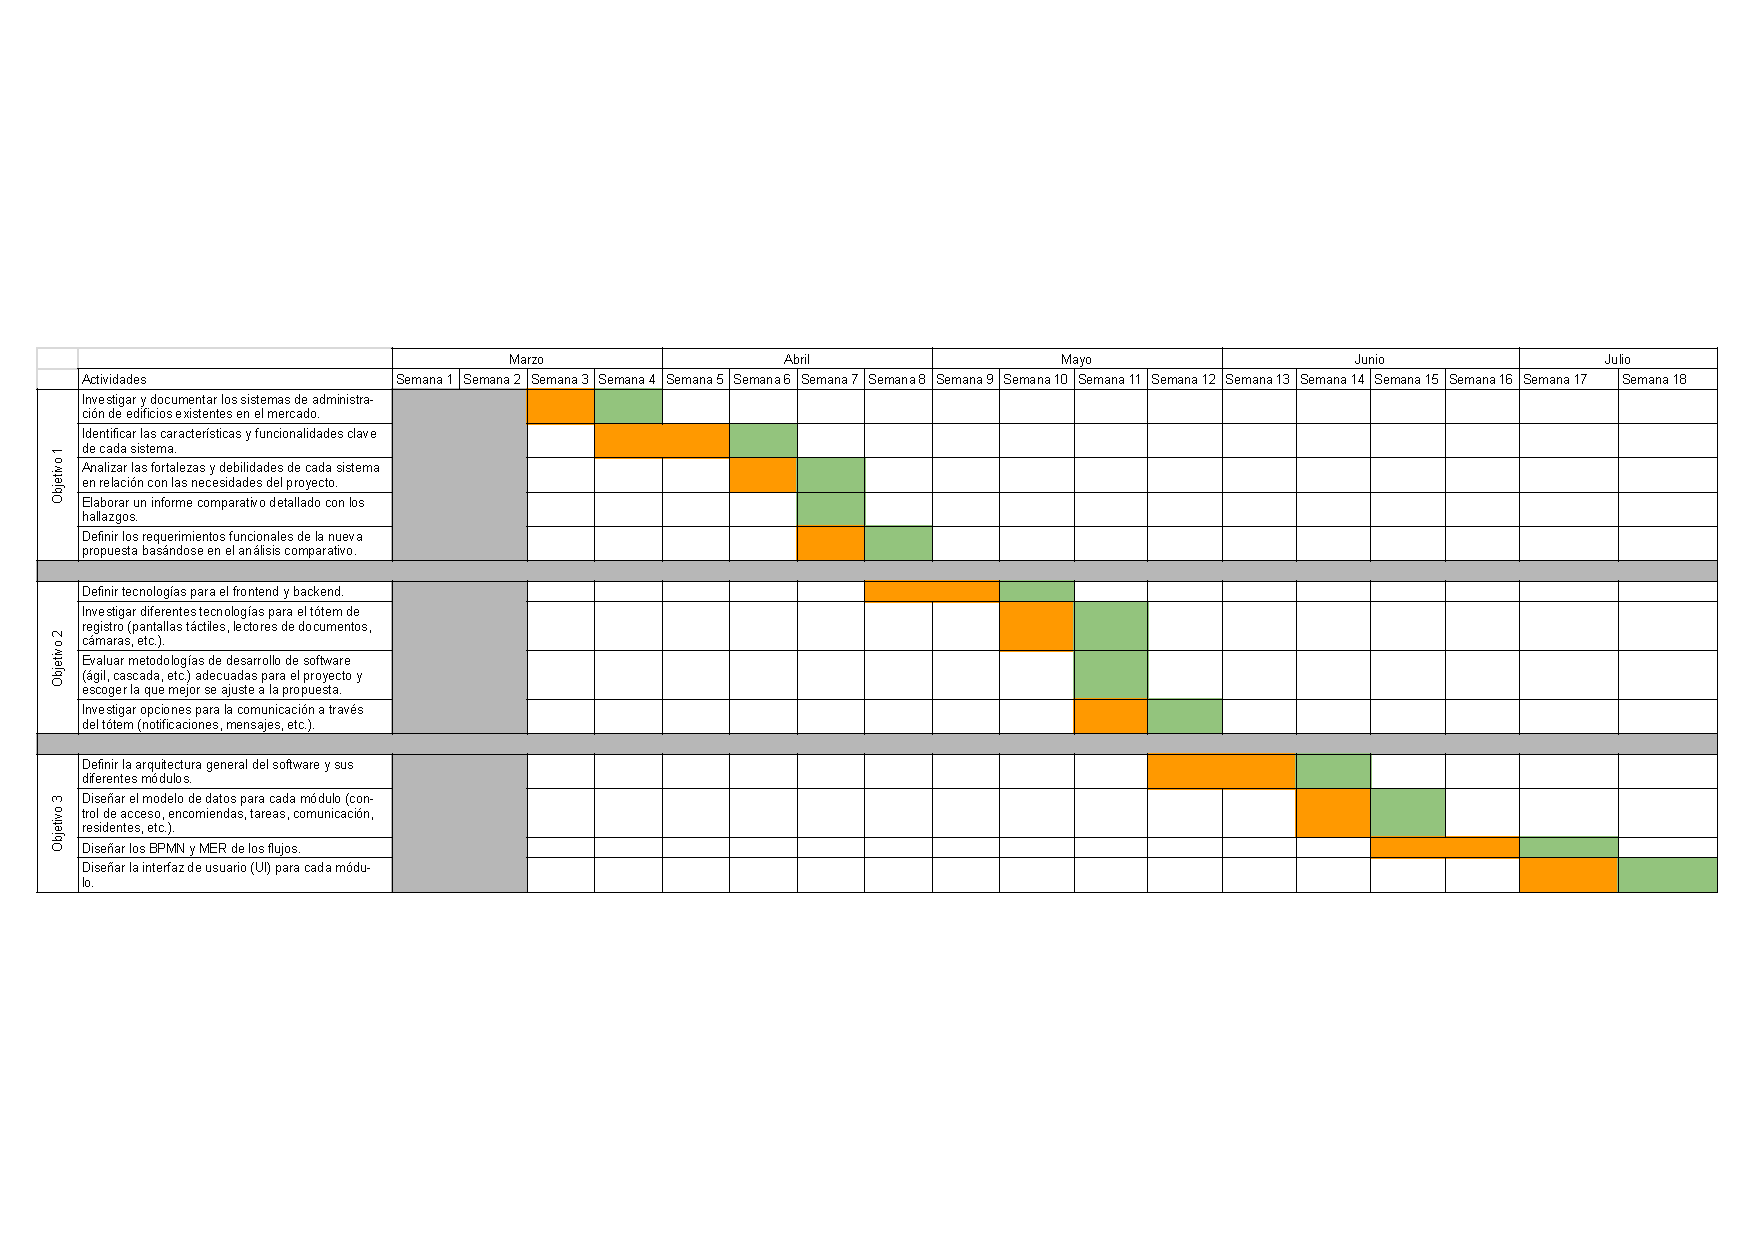
\includegraphics[width=\textheight]{carta-gantt/anteproyecto.pdf}
  \caption{Carta Gantt – Anteproyecto}
  \label{fig:gantt-anteproyecto}
\end{sidewaysfigure}

\begin{sidewaysfigure}[p]
  \centering
  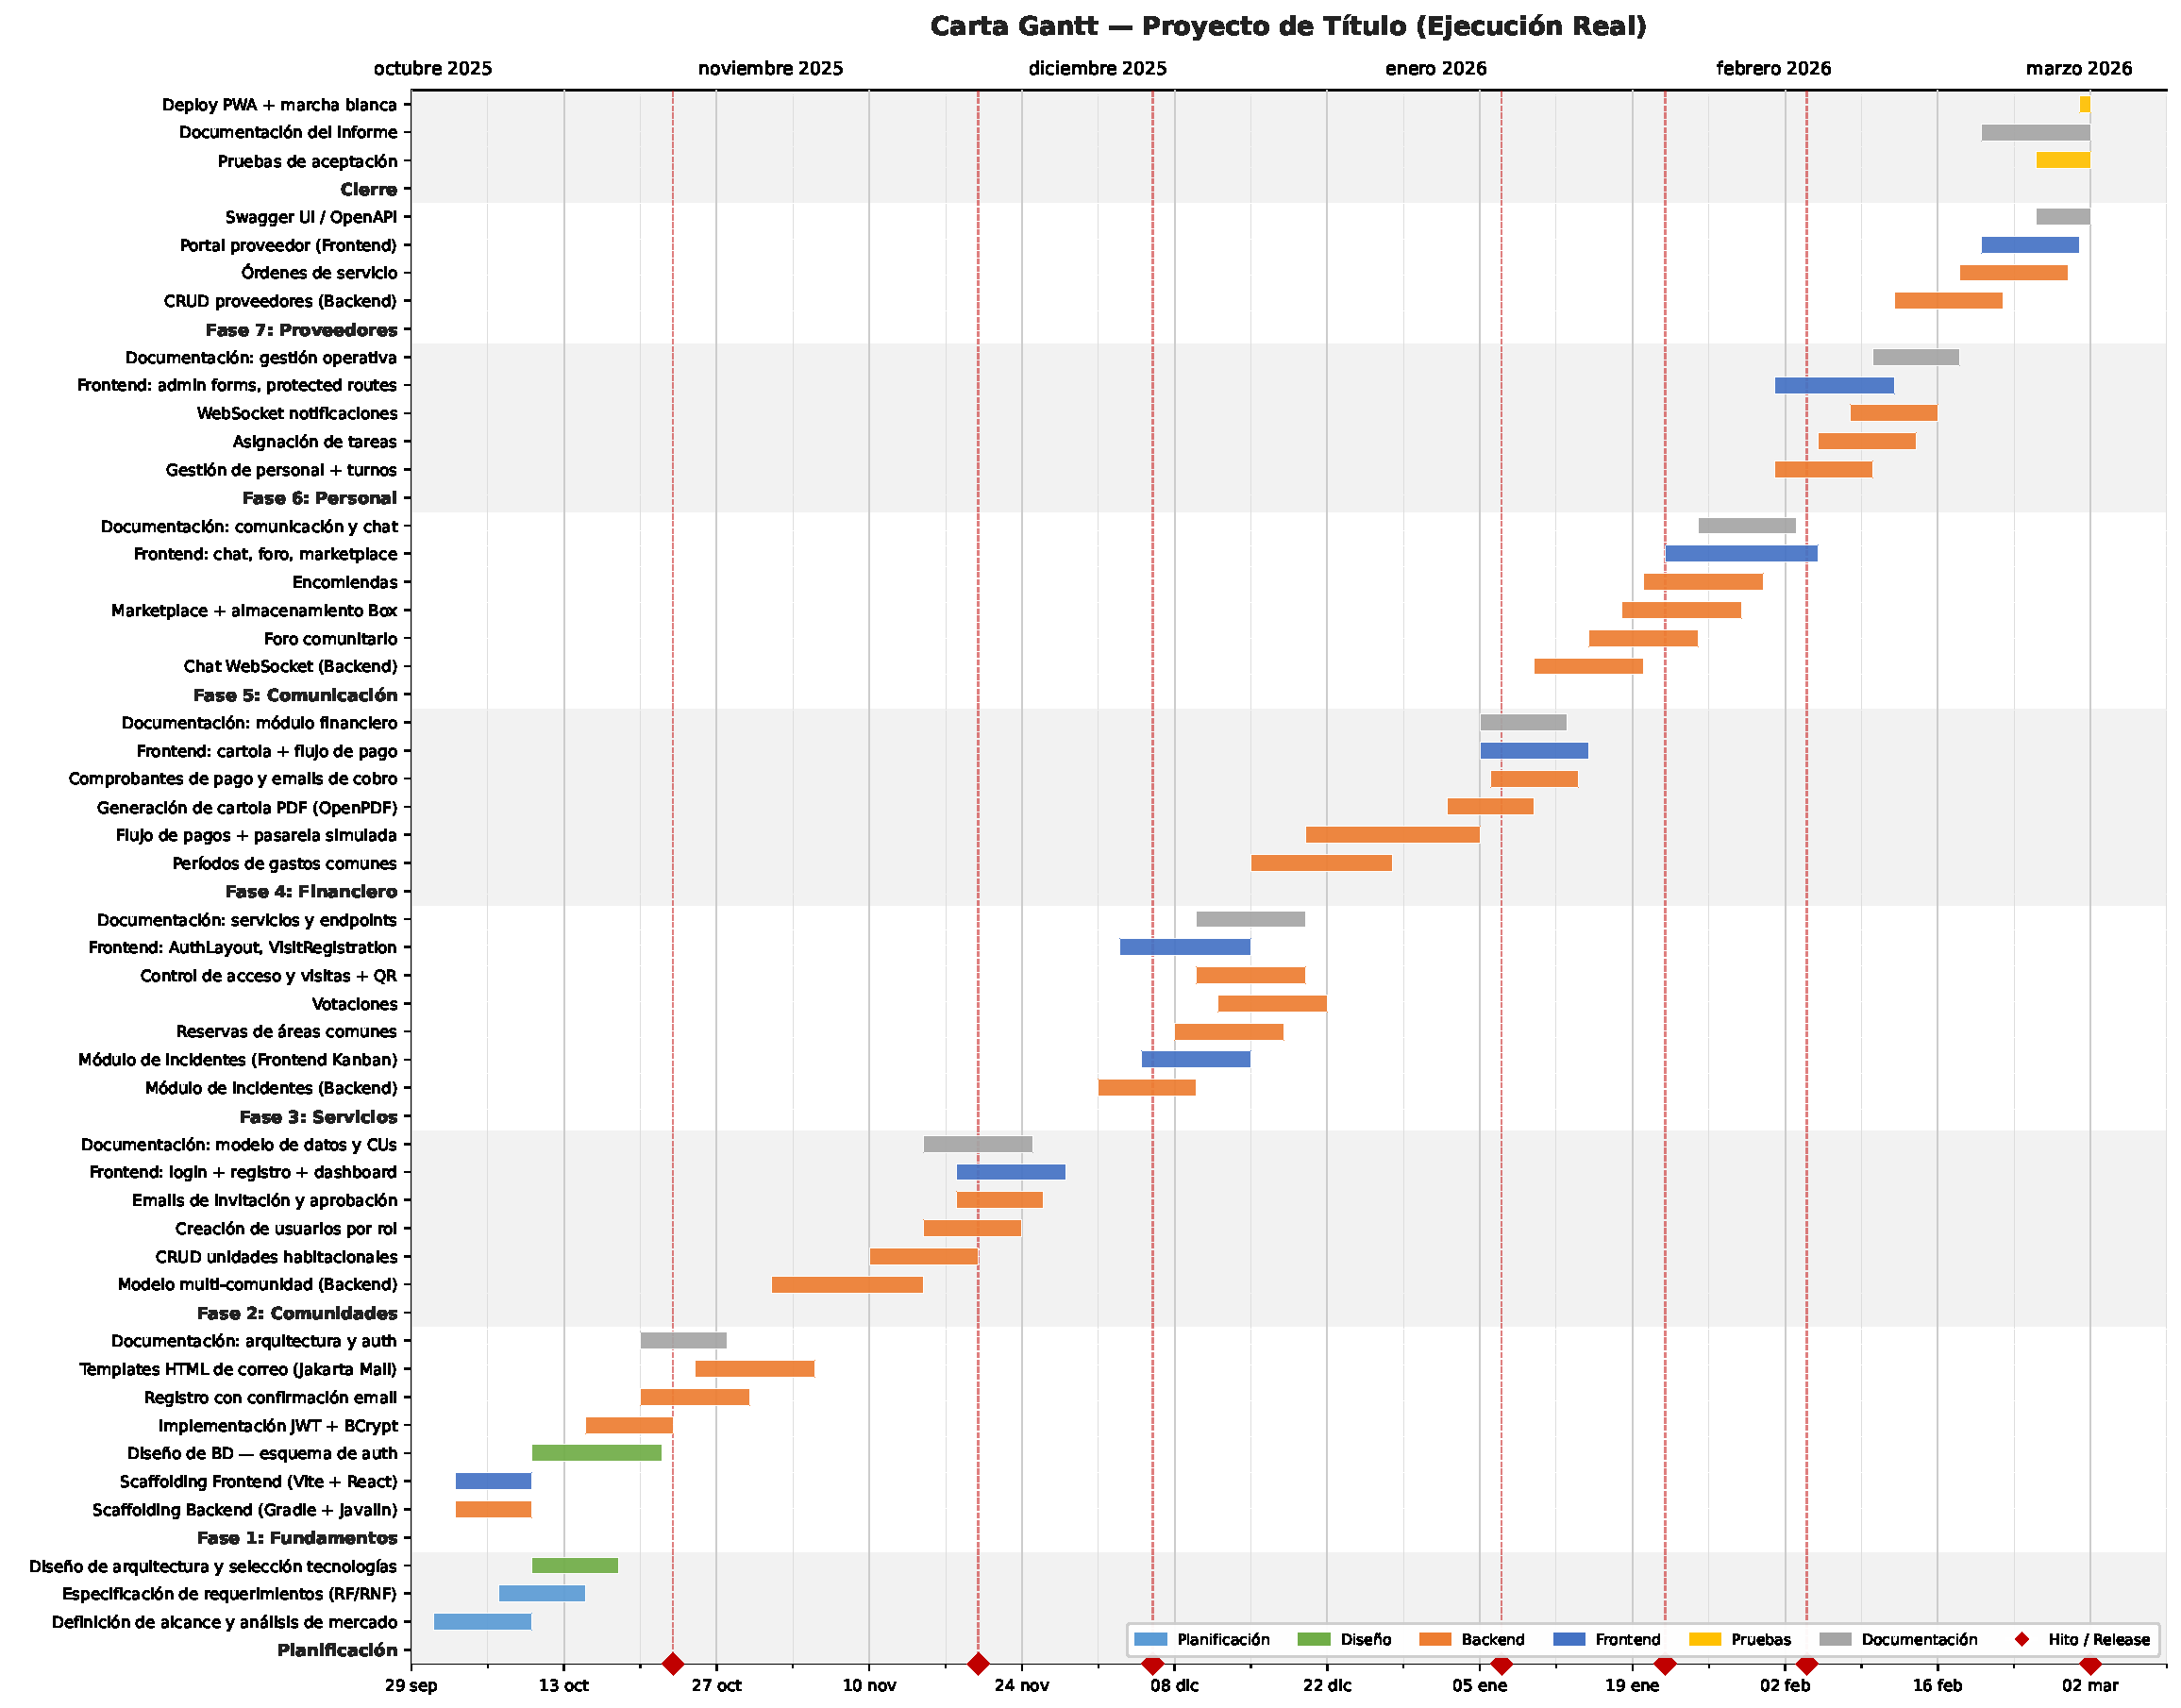
\includegraphics[width=\textheight]{carta-gantt/proyecto.pdf}
  \caption{Carta Gantt – Proyecto de Título}
  \label{fig:gantt-proyecto}
\end{sidewaysfigure}


\end{document}
